\pagebreak
\section{Results}
%\add[XT]{choose some points in the model domain like Choi 2008 did, to monitor the values changes with time (e.g. In VisIt use Query to obtain stress with time for quantatatively analyzing the model behaviors)}
In this ``Results'' chapter, I first walk through the reference model (M28LinT1) and compare it with a constant M model (M88ConT2). Then, I describe in detail the major characteristics of the models. Finally, I describe the effects of different weakening rates, ranges of M variation and functional forms of M variation on the main characteristics.

\subsection{Reference model M28LinT1}\label{sec_M28LinT1}

\begin{figure}[h]
  \centering
    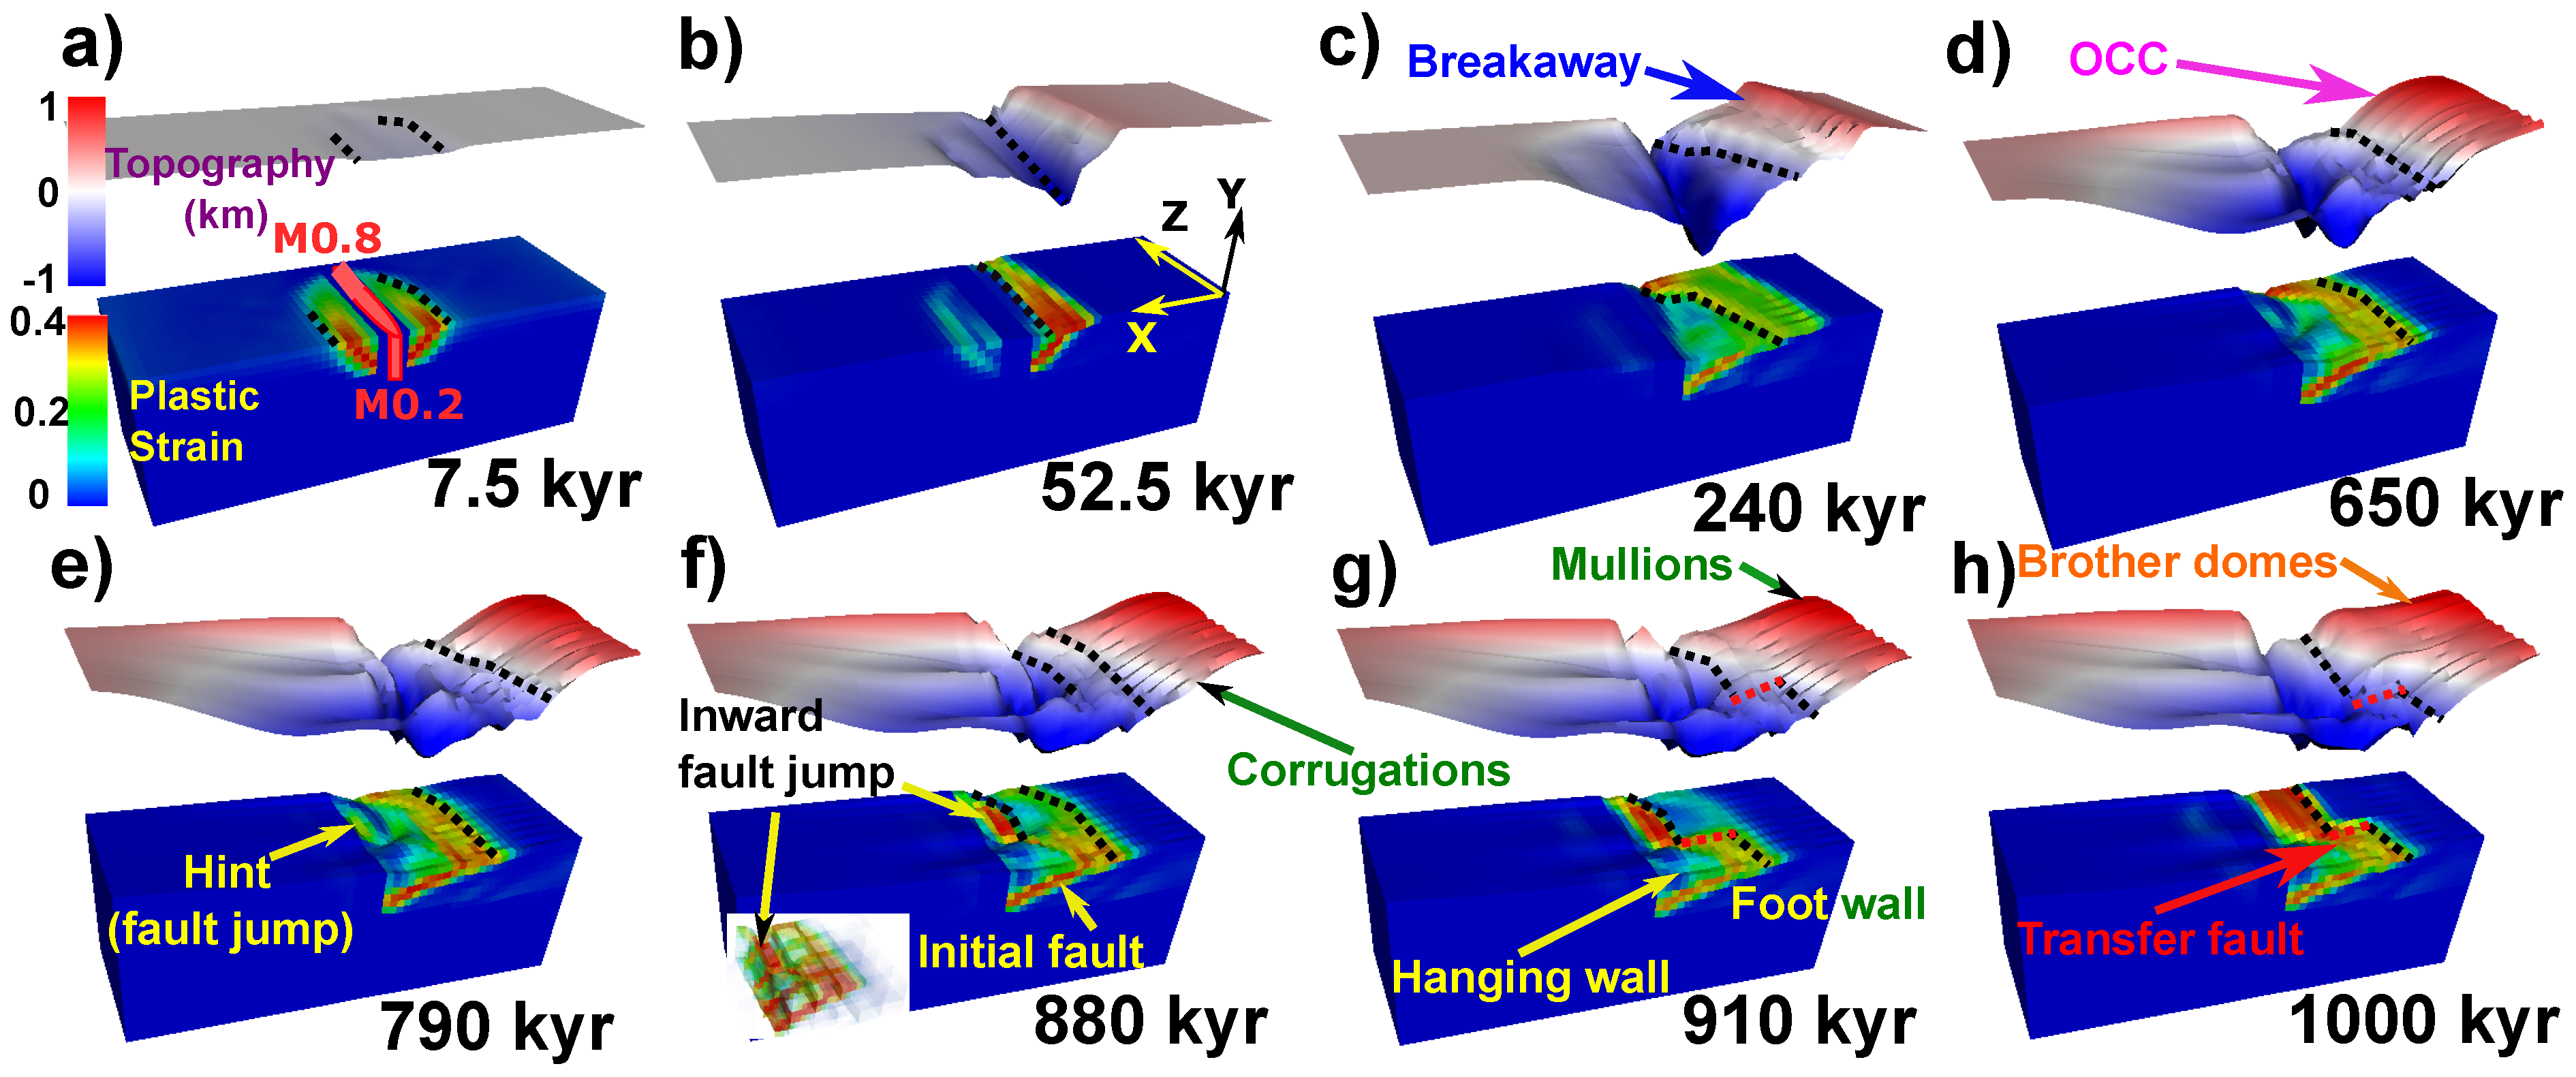
\includegraphics[width=1.0\textwidth]{./Figures/fig_Results_1_reference_model.eps}
  \caption{Evolution of plastic strain and surface topography of the reference model M28LinT1 (Table~\hyperref[Tab1_1]{\ref{Tab1_1}}). Each snapshot shows plastic strain plotted on the model domain and the five times exaggerated topography. Initial seafloor is marked as a reference of 0 km of the topography. The bold dash lines (black) are the terminations of the detachment faults. The bold dash lines (red) in g) and h) are the transfer faults that connect the terminations along the ridge. The inset in f) plots plastic strain with opacity linearly proportional to its value.}%The two insets in b) and d) show $\sigma_{xx}$ (Sxx in the figure) with positive values meaning  tension. The inset in Figure~\hyperref[fig_Results1_1]{\ref{fig_Results1_1}.h} is for shear stress $\sigma_{xz}$ (Sxz in the figure).  The inset in g) also shows velocity vectors.} %Indicated by the velocity vector, the hanging wall of the detachment fault at low M region (M = 0.2$\sim$0.5) is moving in an opposite direction (negative $x$-axis) to its ajacent higher M region (M $>$ 0.5).} %\note[XT]{one thing to be noted is that the $dt=0.5yr$ in these series of 3D models, thus I divided the time step by two to get the time (kyr). This figure needs to be revised that the plastic strain scale is actually changing for different time, a way to revise it is to maintain a constant color scale or attach a color scale for each time. Also, it seems a little bit small and two rows is not as preferable as one row or one column to better express the concept of linear time series evolution.}}
 \label{fig_Results1_1}
\end{figure}   

I consider the model with M varies linearly from 0.2 to 0.8 along the ridge axis with type 1 weakening rate (M28LinT1) as the reference model. The major structural features of the model are indicated in the Figure~\hyperref[fig_Results1_1]{\ref{fig_Results1_1}}. They are breakaway (Figure~\hyperref[fig_Results1_1]{\ref{fig_Results1_1}.c}); oceanic core complex (OCC) (Figure~\hyperref[fig_Results1_1]{\ref{fig_Results1_1}.d}); terminations of the detachment faults where the active faulting interfaces reach the seafloor (black dash line); new high angle normal faults forming near the ridge axis, which is termed as ``inward fault jump'' (Figure~\hyperref[fig_Results1_1]{\ref{fig_Results1_1}.f}); corrugations (Figure~\hyperref[fig_Results1_1]{\ref{fig_Results1_1}.f}) and mullion structures (Figure~\hyperref[fig_Results1_1]{\ref{fig_Results1_1}.g}); and the side-by-side ``brother domes'' (Figure~\hyperref[fig_Results1_1]{\ref{fig_Results1_1}.h}).    

The model produces a median valley that widens and deepens with increasing plate extension (Fig.~\hyperref[fig_Results1_1]{\ref{fig_Results1_1}a-c}). The rate of its widening and deepening at a specific location along the ridge is inversely proportional to the M value (i.e. rate of local magma supply). %OCCs with more than one kilometer in relief and tens of kilometers in wavelentgh are produced. One interesting behavior worth noting is that corrugations with wavelengths of hundred-to-thousand meters and amplitudes of ten-to-hundred meters are also produced.

For the first 7.5 kyr (Figure~\hyperref[fig_Results1_1]{\ref{fig_Results1_1}.a}), %high angle ($\sim$60 $\degree$)
normal faults, represented by localized plastic strain, begin to form near the ridge axis.
%The angles of the faults are consistent with  Anderson's theory of faulting mechanics for a frictional angle of 30 $\degree$.
Because stresses due to plate motions accummulate faster at the lower M side than at the higher M side, faults first initiate at the lower M side and then propagate to the higher M side. The asynchronous initiation of faults along the ridge axis creates offset in breakaway: i.e., the breakaway at the lower M side extends further than that of the higher M side (Figure~\hyperref[fig_Results1_4]{\ref{fig_Results1_4}}).
%The along-ridge coupling forces (i.e. torsion (clockwise); shearing ($\sigma_{xz}$)) prevent relative displacement between the two neighbors along the ridge axis. These along ridge coupling forces on the other hand assist in fault propagation from the lower M side (M = 0.2) to the higher M side (M = 0.8) and reduces the time difference in the initiation of faulting along the ridge axis when comparing with seperated pseudo-2D models.

\begin{figure}[h]
  \centering
    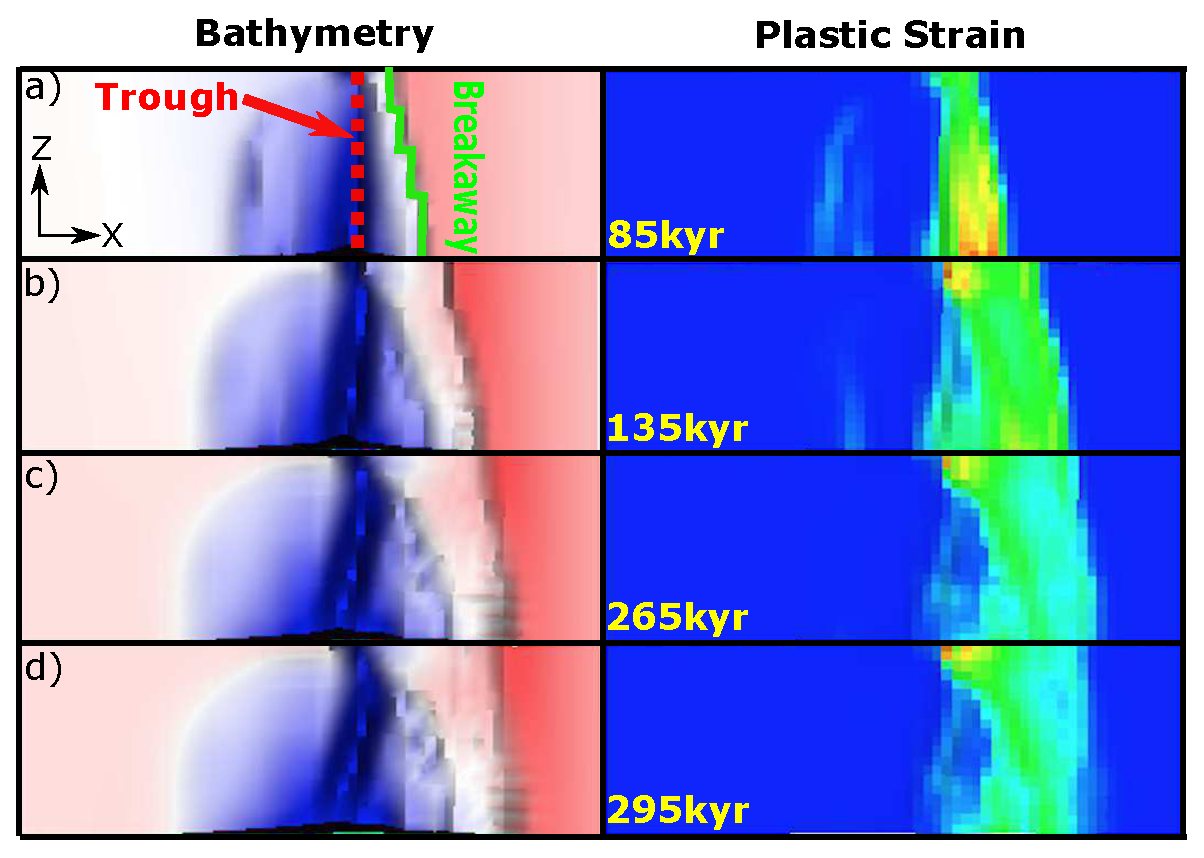
\includegraphics[width=0.6\textwidth]{./Figures/fig_Results1_4.eps}
  \caption{Bird's-eye view of the evolution of breakaway (marked by green bold line) and depressed narrow zone (``axial trough'') along the ridge axis (red dash line in (a)) for model M28LinT1 (Table~\hyperref[Tab1_1]{\ref{Tab1_1}}). This figure share the same color scales with Figure~\hyperref[fig_Results1_1]{\ref{fig_Results1_1}}.}
 \label{fig_Results1_4}
\end{figure}

\begin{figure}[h]
  \centering
    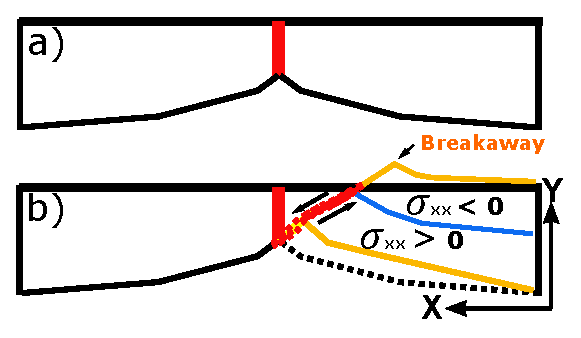
\includegraphics[width=0.6\textwidth]{./Figures/fig_Results4_8_sqrt_cut_back_bending_cartoon.eps}
  \caption{Bending stress illustration. The blue line is the neutral plane where $\sigma_{xx}=0$. Above the neutral plane is compression ($\sigma_{xx}<0$) and beneath it is tension ($\sigma_{xx}>0$).}
 \label{fig_Results4_8}
\end{figure}

By 52.5 kyr (Figure~\hyperref[fig_Results1_1]{\ref{fig_Results1_1}.b}), the normal fault on the right hand side of the ridge axis remains active while the one on the left becomes inactive. 
%The choice of which fault to survive seems determined by a small numerical perturbation between the two faults seen in Figure~\hyperref[fig_Results1_1]{\ref{fig_Results1_1}.a} although the model setup is symmetrical across the ridge axis. 
As the fault evolves, the upper part of the permanent deformed interface (shown as plastic strain in the model) of the fault is exhumed to the seafloor with its front edge extending away from the ridge axis following the spreading plate. Initially, the extending edge of this fault interface corresponds to the right boundary of the plastic strain along the ridge. Note that the extending boundary (tips) of the plastic strain also aligns with the breakaway along the ridge before 265 kyr (Figure~\hyperref[fig_Results1_4]{\ref{fig_Results1_4}.a$\sim$c}).\add[XT]{The previous sentence is for explaining the extending tips of plastic strain} The along-ridge offset in $x$-direction of the tips of the extending plastic strain reduces at $\sim$295 kyr (Figure~\hyperref[fig_Results1_4]{\ref{fig_Results1_4}.d}) because when the normal fault lasts long enough and bends to a low angle detachment fault at the lower M side, the termination of the detachment fault stops extending and the healing of plastic strain (following \citealp{Tucholke2008}) implemented in the model reduces quickly the plastic strain of the inactive fault interface that has been exhumed to the seafloor. While at the higher M side, the termination keeps extending and reduces the initial offset generated by the asynchronous initiation of faulting. In addition, as the fault slips, crust at the footwall bends in a clockwise rotation as illustrated by Figure~\hyperref[fig_Results4_8]{\ref{fig_Results4_8}}. %The neutral plane ($\sigma_{xx}=0$) is shown as the boundary between blue (compression) and pink (tension) (inset of Figure~\hyperref[fig_Results1_1]{\ref{fig_Results1_1}.b}). 


%the fault displacement at the front side is larger than that of the back because M is lower at the front and more extension needed to be accommodated by the tectonic processes (i.e. normal faulting). \annote[XT]{Thus, the breakaway at the front extending further away from the ridge axis.}{I am not sure whether the breakaway extends further at lower M side because it should be the same. The breakaway at lower M side does extend further not because of fault slip rate difference but becauses of initiation time, at lower M side, fault begin earlier thus the breakaway begin to extend earlier and reach further, however, the rate of extending away from axis for the breakway should equal to the extension rate $V_{x}$. Thus the offset between breakaways of front and back remains constant} The termination of the detachment fault where footwall begins to be exhumed to the surface will extend further due of faster bending of the footwall at the lower M side. This will also result in a larger volume of exhumation at the lower M side than that of the higher M side. For our model that even when $M=0.2$, the detachment fault can still last for a long time \citep{Baines2008}, the exhumation rate has a upper limit of extension rate of $V_{x}$ in spite of a higher fault slip rate at lower M side.  

%The termination of the detachment fault at the lower M side (M $<$ 0.3) is at $\sim$15km from the ridge axis 
The active, near-axis normal fault rotates to a lower dip of $\sim$30 $\degree$ at the root of the fault and to $\sim$0 $\degree$ at the exposed fault interface (Fig.~\hyperref[fig_Results1_1]{\ref{fig_Results1_1}.c}). However, the normal fault at the higher M side (especially for M $>$ 0.7) experiences less bending and the termination of the fault is closer to the ridge axis. The maximum relief between the breakaway and the axial trough inside the median valley becomes larger than 1 km. In addition, $\sim$1 km wavelength corrugations begin to show up between the breakaway and termination on the lower M side (M $<$ 0.3). The corrugations show a uniform wavelength, which is also smaller than that of the mullion structures (Figure~\hyperref[fig_Results1_1]{\ref{fig_Results1_1}.g}). Formation mechanism for these structures are discussed in one of the following sections. The axial trough is initially straight and parallel to the ridge axis (Figure~\hyperref[fig_Results1_4]{\ref{fig_Results1_4}.a}) but becomes oblique to the ridge axis. The obliquity increases with the amount of extension (Figure~\hyperref[fig_Results1_4]{\ref{fig_Results1_4}.b,c,d}). 

By 650 kyr (Figure~\hyperref[fig_Results1_1]{\ref{fig_Results1_1}.d}), the median valley becomes wider and deeper. The detachment fault reaches its lowest dip angle and its termination stops moving away from the ridge axis. The breakaway of this detachment has already moved out of the model domain.
%\annote[XT]{moved out of the model domain}{it should not, if breakaway move with 25km/yr(half spreading rate), since the distance between initial break (5km away from ridge center) and right wall of the model domain is about 25km which needs 1Myr to reach. But now is only 650 kyr. Why is it?}.
The total fault offset at this point is greater than the thickness of the crust and thus sufficient for exhuming the upper mantle materials. %The previous fault interface bends over and dips away from the ridge axis, producing a cylindrical OCC. 
A hint of the inward fault jump appears up over the area corresponding to 0.5 $<$ M $<$ 0.65.
%\add[XT]{Its formation will be discussed in Discussion section accompanied by the stress status analysis. }

By 790 kyr, a new near-axis fault appears and propagates toward the high M ($>$ 0.5) side (Fig.~\hyperref[fig_Results1_1]{\ref{fig_Results1_1}.e}). However, the initial detachment fault is still active and takes up most of the extension. The distance between the termination of the detachment fault and the ridge axis is greater at the lower M side.%because the detachment fault at the higher M side remains in higher dip angle due to less fault slip. %This along ridge variation produces three type 2 corrugations (it will be further explained in the next section). One has a wavelength of $\sim$6 km with an amplitude of several hundred meters. The other two are on the surface of the first corrugation with wavelengths of less than 1 km and amplitudes of several tens of meters.   
Subsequently, the detachment fault becomes less active and the new near-axis fault accommodates most of the intra-plate extension. This event is called the ``inward fault jump'' [\citealp{Tucholke1998}; \citealp{Dick2008}]. The new high angle normal fault cuts through the hanging wall of the detachment fault (Fig.~\hyperref[fig_Results1_1]{\ref{fig_Results1_1}.f}). %However, it still coexists with the initial detachment fault (shown in the inset). 

\begin{figure}[h]
  \centering
    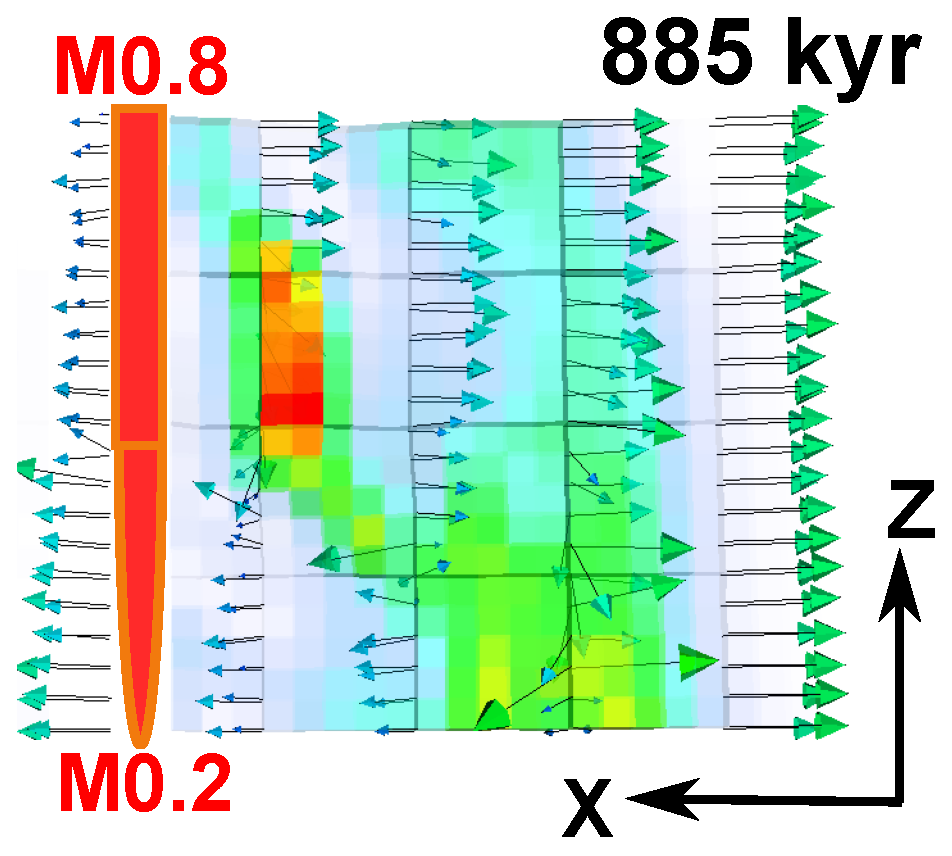
\includegraphics[width=0.5\textwidth]{./Figures/fig_Results_1_velocity_field.eps}
  \caption{Bird's-eye view of velocity field with plastic strain ploted with \annote[EC]{opacity}{why do you need tranparency in this figure?} \add[XT]{if not transparent, the velocity vectors will be hidden} linearly proportional to its value. (color scale is the same as Figure~\hyperref[fig_Results1_1]{\ref{fig_Results1_1}.a)})}
 \label{fig_Results_1_velocity_field}
\end{figure}

\begin{figure}[h]
  \centering
    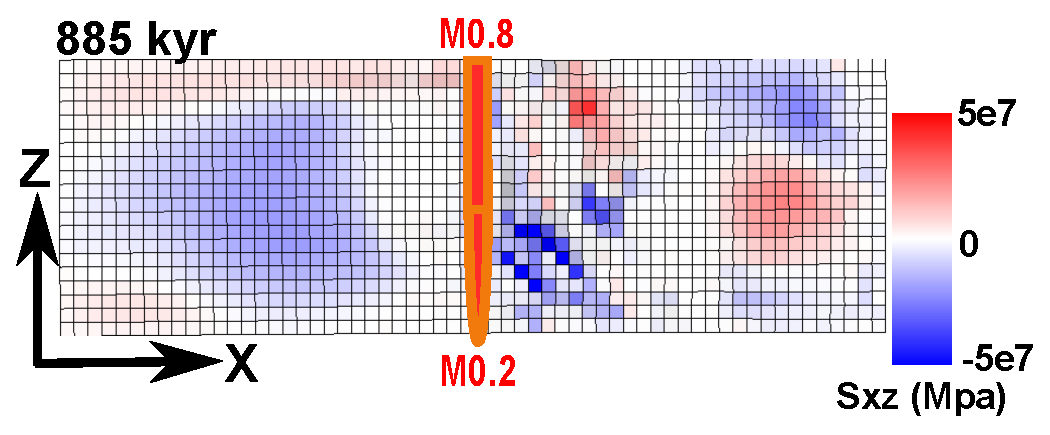
\includegraphics[width=0.8\textwidth]{./Figures/fig_Results_1_Sxz.eps}
  \caption{Bird's eye view of $\sigma_{xz}$.}
 \label{fig_Results_1_Sxz}
\end{figure}

By 910 kyr (Fig.~\hyperref[fig_Results1_1]{\ref{fig_Results1_1}.g}), the inward fault jump completes in the M $> 0.5$ region: the new high-angle fault takes up all the extension and the initial detachment fault becomes completely inactive. The block that was previously a hanging wall to the detachment becomes footwall of the new fault and moves with the spreading plate to the positive $x$-axis direction. At the lower M side, the detachments is still active and the hanging wall continues to move toward the negative $x$-axis direction (Figure~\hyperref[fig_Results_1_velocity_field]{\ref{fig_Results_1_velocity_field}}). This opposite sense of relative motions between the high and the low M side creates a region of \annote[EC]{dextral}{Isn't it sinistral?} shear and eventually creates a transfer fault (Fig.~\hyperref[fig_Results1_1]{\ref{fig_Results1_1}.h}). %at the lower M side (M $<$ 0.5) $\sim$45 $\degree$ oblique to the ridge axis (Figure~\hyperref[fig_Results_1_Sxz]{\ref{fig_Results_1_Sxz}}) and the shear stress zone produces a new trough inside the median valley that aligns with it. Combined with the previous trough, an ``X'' shape topography low is created in the model.


\subsubsection{Constant M model M88ConT2}

\begin{figure}[h]
  \centering
    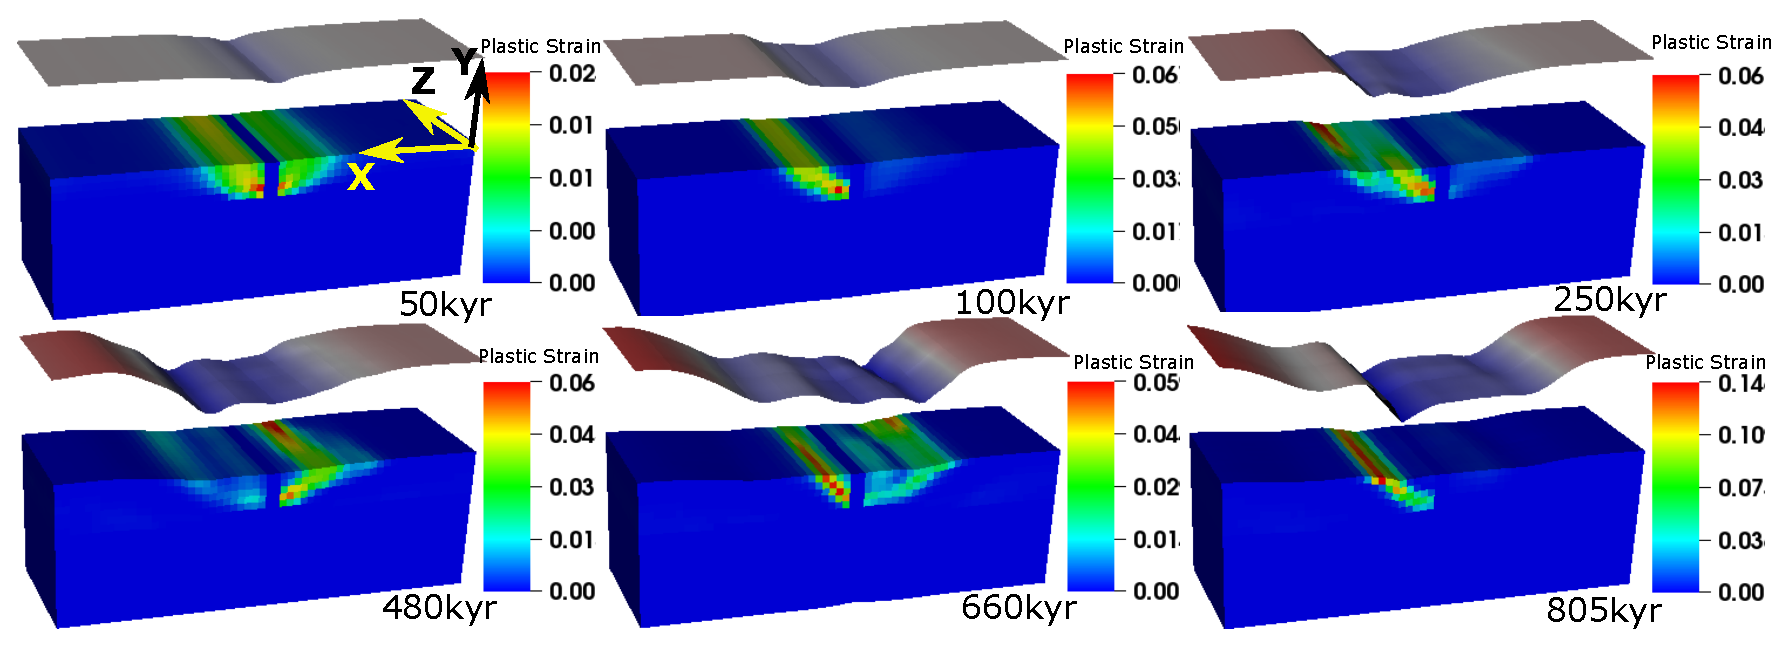
\includegraphics[width=1.0\textwidth]{./Figures/fig_Results1_3.eps}
  \caption{Evolution of plastic strain and surface topography of the model: M88ConT2 (Table~\hyperref[Tab1_1]{\ref{Tab1_1}}). (color scale of topography is the same as Figure~\hyperref[fig_Results1_1]{\ref{fig_Results1_1}.a})}
 \label{fig_Results1_3}
\end{figure}   

As a comparison to the varying M models, a constant M model is run. 

As shown in Figure~\hyperref[fig_Results1_3]{\ref{fig_Results1_3}}, model M88ConT2 pruduces a $\sim$20 km wide and 1$\sim$2 km deep median valley, which is similar to the generally observation of the Mid-Atlantic Ridges. The width and depth of the median valley is almost constant along the ridge as contrast to the varying M models. The variation of the location of the breakaway and termination along the ridge that is mentioned in the reference model (M28LinT1) does not show up. Because the magma supply is constant along the ridge with M = 0.8, there is no stress perturbation along the ridge. Thus, the normal faults along the ridge initiate at the same time and the slipping rate of the fault is also constant along the ridge axis. The synchronized fault initiation results in no offset between breakaways and the constant sliping rate produces no along ridge axis variation in the position of the termination. In addition, neither corrugations nor mullion structures are generated. Normal faults alternate on each side of the ridge axis with a period of $\sim$300 kyr due to the mechanism metioned in the ``Introduction'' section for the 2D models of M $>$ 0.5. This fault alternaltion produces symmetrical high frequncy abyssal hills. For 3D models, why and how fault alternates on each side of the ridge axis is different from the previous 2D studies and is described in the following sections. 

\subsection{Main characteristics of the models}
I identify seven features that are common to most of the models: location of the termination, geometry of the trough, inward fault jump, fault alternation, mass wasting, hourglass-shaped median valley and corrugations and mullion structures. Since the details of these features differ among the models, they are useful for delineating and contrasting complicated model behaviors.

\subsubsection{Location of \annote[EC]{termination}{I think ``fault trace'' is what you mean.}}
\add[XT]{for the term ``termination'' please refer to:}
23 times usage from \citep{Canales2008} or
 \citep{Blackman2009} or
 figure one of \citep{Dick2008} or
 figure six of \citep{Mallows2012} or
 figure 1,2,3A of \citep{Schouten2010} 
But \citep{Reston2011a} give a further discussion on it and they favor ``top hanging wall cutoff''.
they also mention that ``The traditional map term fault trace, which is not generally used on sections, is not appropriate as it cannot be used to describe the geometry of a structure everywhere buried by later sedimentary rock.''
\begin{figure}[h]
  \centering
    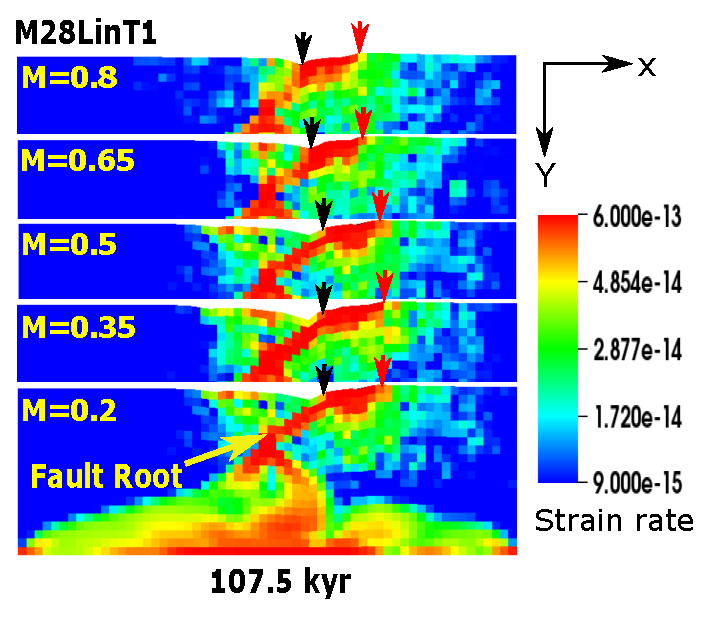
\includegraphics[width=0.6\textwidth]{./Figures/fig_Results1_2.eps}
  \caption{The second invariant of strain rates plotted on the reference model's vertical cross-sections along the ridge at 107.5 kyr. Terminations and breakaways are marked by black and red arrows.}
 \label{fig_Results1_2}
\end{figure}   

The location of a fault trace is delineated by black dashed lines in Figure~\hyperref[fig_Results1_1]{\ref{fig_Results1_1}} and marked by black arrwos in Figure~\hyperref[fig_Results1_2]{\ref{fig_Results1_2}}.
%As shown in Figure~\hyperref[fig_Results1_2]{\ref{fig_Results1_2}}, the highest strain rate regions (red) can be interpreted as the active detachment fault interfaces. 
The reference model shows that distance from the ridge axis to \change[XT]{fault trace}{the termination of the detachemtn fault} is greater on the lower M side than on the higher M side because faulting starts on the lower M side first and initiates later on the higher\add[XT]{I have been using higher M side and lower M side instead of high or low M side} M side.
%Because the distance between the termination and the fault root is smaller at the higher M side, the dip angle of the fault is higher. 
%Among the three slices of M $<=$ 0.5, the distances and the dip angles are similar. Because although the rate of fault slip is higher for lower M, the rotation rate of the detachment fault interface is determined by how fast the termination extends away from the fault root. This is because the detachment faults for the ridge region of M $<$ 0.5 root at the same place at the intersection between the center dike and the brittle-ductile transition (BDT). Since the extending rate of the termination has a maximum value that is restricted by the far field extension rate $V_{x}$, the bending rates of the detachment faults is similar among the three slices of M $<=$ 0.5.  %In other words, in order to spend least frictional energy during faulting, the detachment fault interface between the two ends (termination and fault root) tends to be a straight line.     Thus, the dip angle of the detachment fault is inversely proportional to the distance between the termination and the root of the fault when M $<$ 0.5. Since the breakaways at the lower M side (M $<$ 0.5) moves with the extending plate under the same velocity $V_{x}$, and the initiation time difference of the normal faults at the lower M side is similar (Figure~\hyperref[fig_Results1_1]{\ref{fig_Results1_1}.a}), the distances between the breakaways and the roots of the faults are the same. Meanwhile, the distance between breakaways and terminations as indicated by the red and black arrows in the Figure~\hyperref[fig_Results1_2]{\ref{fig_Results1_2}} is similar along the ridge axis. Thus the dip angles of the faults at the same time along the ridge-axis are very much the same. However, when M $>$ 0.5 (Figure~\hyperref[fig_Results1_2]{\ref{fig_Results1_2}, (M = 0.65, 0.8)}), the amount of fault slip decreases as M increases. The crust at the footwall experiences less bending and the detachment fault remains in a higher angle as well as that the terminations are closer to the ridge axis. Because the root of the fault is slowly pushed away from ridge axis while the breakaways of the faults are closer to ridge axis due to a later initiation of the fault. In addition, the crust thickness that the fault cuts through is slowly increasing as the fault being pushed away from ridge center due to excessive diking. These three factors together contribute to a higher dip angle. In a unit time, the volume of the exhumation is also smaller for the higher M side.
%One thing needs to be noted is that the trough at the higher M side correspond to the terminations but detached from the terminations at the low M side (M $<$ 0.5) as shown in Figure~\hyperref[fig_Results1_2]{\ref{fig_Results1_2}}.

\subsubsection{Geometry of axial trough}
%\subsubsection{Shear low (M28LinT1)}

The depressed narrow region inside the median valley is termed as ``trough''\note[EC]{In my opinion, ``axial trough'' would be better}.\add[XT]{However, axial trough is usually used for fast spreading and axial sounds like on the central axis of the ridge, However, this trough describing here is for the lowest points insdie the median valley of slow spreading ridge that can become a curve and be off the axis } The reference model showed that its shape in the map view evolves from a straight line parallel to the ridge axis to a line oblique to the ridge-axis (Figure~\hyperref[fig_Results1_4]{\ref{fig_Results1_4}}). Initially, the trough corresponds to the fault trace. As the normal fault rotates to a lower dip on the lower M side, the trough is no longer coincident with the fault trace. %Also, the trough at the lower M side is pulled to the conjugate plate to the negative $x$-axis direction. 
The axial trough on the higher M side (M $>$ 0.5) are pushed away from the ridge axis \citep{Tucholke2008}. However, since \annote[EC]{the trough cannot bypass the termination}{What do you mean?}\add{the trough is to the side which is nearer to the ridge axis than termination, it cannot bypass termination further away from the ridge axis}, the trough at M = 0.8 is restricted at the termination. Together it generates the curved trough (Figure~\hyperref[fig_Results1_4]{\ref{fig_Results1_4}}). 
%{Important tecnique from discussion on Mar. 9th with Eunseo: 1. One way to analyze models is to make hypothesis to describe model behaviors and than use models to approve or reject it. If rejected, find a new hypothesis and do the same thing again.}
%\add[XT]{4. An new thinking on little termination or dip angle variation when M$<0.5$ as observed in %figure~\ref{fig_Results1_2}: why along-z hanging wall has little variation is because we have along z coupling, the rotational shear failure between along-z neighbors are so hard. and also, the more extension in M0.2 end is accommodated elastically by the whole plate to the left of the detachment fault which can be observed as lower topo(topography variation along ridge axis).} 
%\add[XT]{One question needs to be answered: at 410 timesteps (205kyr), the breakaway at the front already extends 15km. If assumming a constant extending rate, it means a velocity of around 75km/Myr, much faster than half spreading rate 25km/Myr. If it is true, I need to change previous discussion on how fast breakaway being pulled away from ridge-axis.}


\subsubsection{Inward fault jump}
The inward fault jump occurs in all the models when an old fault locks and a new one forms near the ridge axis (e.g., Fig.~\hyperref[fig_Results1_1]{\ref{fig_Results1_1}}).
%, at the region with M $>$ 0.5, the existing normal fault is pushed away from the ridge-axis due to \annote[EC]{excessive}{Doesn't sound appropriate. Probably you mean, ``frequent''.} diking (Figure~\hyperref[fig_Results1_1]{\ref{fig_Results1_1}.c,d}). As it moves away from the ridge axis, the \annote[EC]{frictional energy}{What do you mean?} for the fault, the bending energy for the footwall as well as the \annote[EC]{negative}{What do you mean?} work done by gravity that resists the exhumation of the footwall increase [\citealp{Lavier2000, Olive2014}]. The initial detachment fault remains active until the negative works reach an upper limit that breaking a new fault near the ridge axis needs less work than to maintain the initial one, the initial detachment fault at the higher M side is substituted by the inward jumping fault that cuts through the previous hanging wall. This inward jumping behavior of the normal fault is termed as ``inward fault jump''.
\add[XT]{for the description of the previous commented out paragraphy, please refer to:}[\citealp{Lavier2000}; \citealp{Olive2014}]

The new fault usually forms on the high M side first and it connects to the existing detachment developing on the lower M side (M $<$ 0.5), creating a curved fault trace. Unlike fault alternation, the inward fault jump occurs on the same side of the ridge axis and its along-axis extent corresponds to the M $>$ 0.5 region. %rather than cut through the whole MOR segment.

\subsubsection{Fault alternation}
When M is high enough, a normal fault first forms on one side of the ridge axis but another fault forms on the other side when the first one locks (Fig.~\hyperref[fig_Results1_3]{\ref{fig_Results1_3}}) \citep{Buck2005,Tucholke2008}. This behavior is termed as ``fault alternation''. %Among the 12 models (Table~\hyperref[Tab1_1]{\ref{Tab1_1}}), only three models produces fault alternation. They are M88ConT2, M58SinT2 and M58SqrtT2. Fault alternates only when weakening rate is low (type 2 weakening) and the average integration of M along the ridge is larger than 0.65. Analysis on when and why fault alternates is given in ``Discussion'' section.

\subsubsection{Cut-back}\label{para_CutBack} \add[XT]{How about change Cut-back to shear-wasting or mass wasting or cut-wasting}\note[EC]{Mass wasting sounds most appropriate.}

\add[XT]{For ``shear-wasting'', shear is from the three triggering shear stresses, wasting is from mass wasting. For mass wasting, it has the benefit that people are familiar with this term, however, the new mechanism for triggering it(the shear stress) is missing}\note[EC]{Didn't we agree that shear stress seen in the vertical cross-section does not trigger this event?}

\begin{figure}[h]
  \centering
    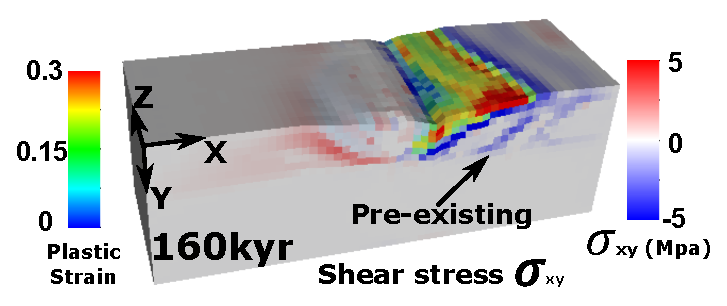
\includegraphics[width=0.6\textwidth]{./Figures/fig_Results4_5_sqrt_cut_back_pre_accummulated_shear_zone.eps}
  \caption{The weak detachment fault tip reaches the pre-existing shear stress. Plastic strain is plotted with opacity linearly proportional to its value.}
 \label{fig_Results4_5}
\end{figure}   

\begin{figure}[h]
  \centering
    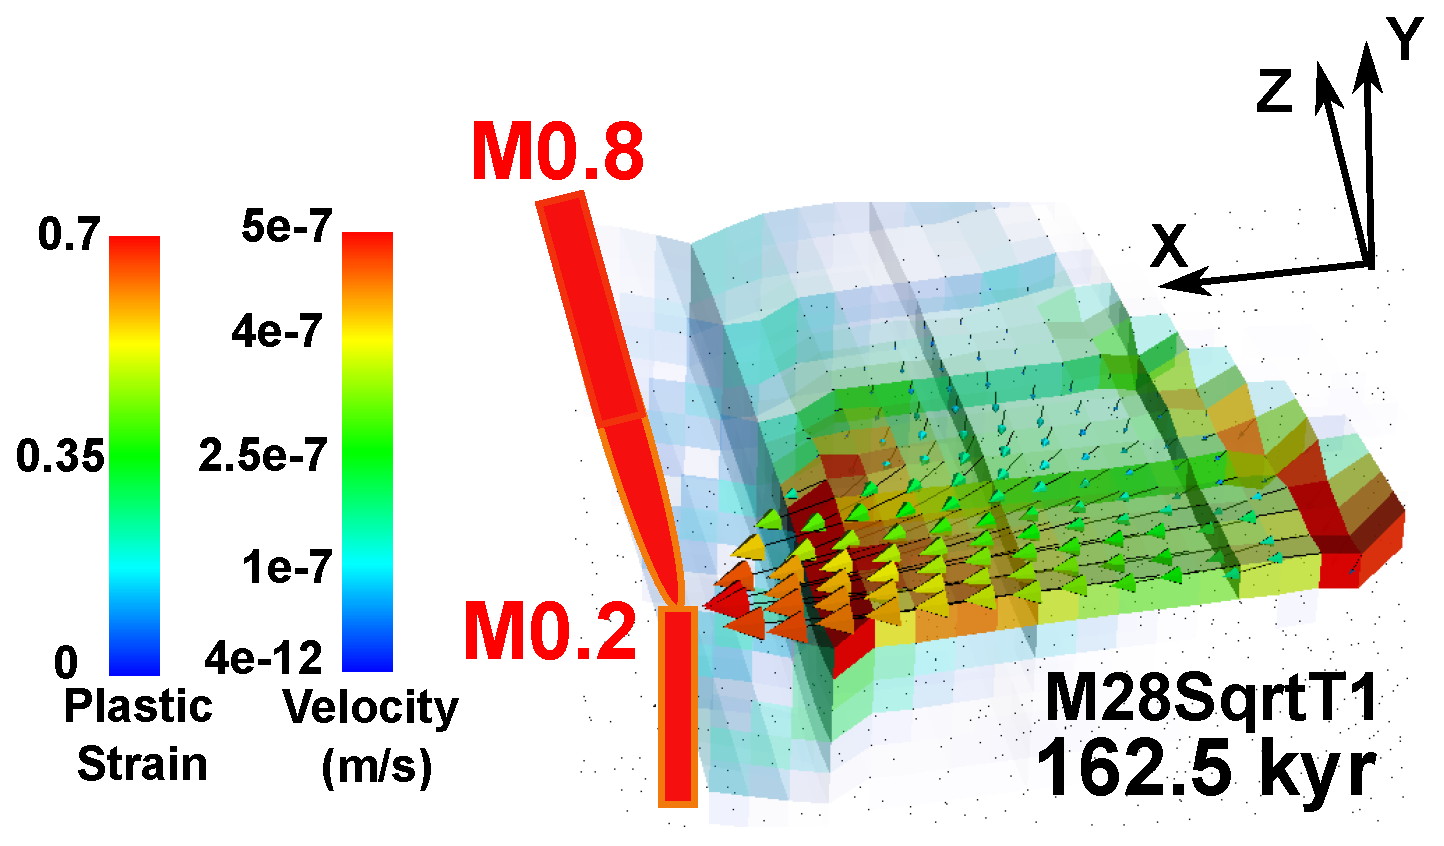
\includegraphics[width=0.6\textwidth]{./Figures/fig_Results_3_2_5_Cut-back_velocity.eps}
  \caption{Velocity of the mass wasting hanging wall. Magnitudes of the velocity are shown by the colors of the arrow heads. Plastic strain is plotted with opacity linearly proportional to its value.}
 \label{fig_Results_3_2_5_Cut-back_velocity}
\end{figure}   

\begin{figure}[h]
  \centering
    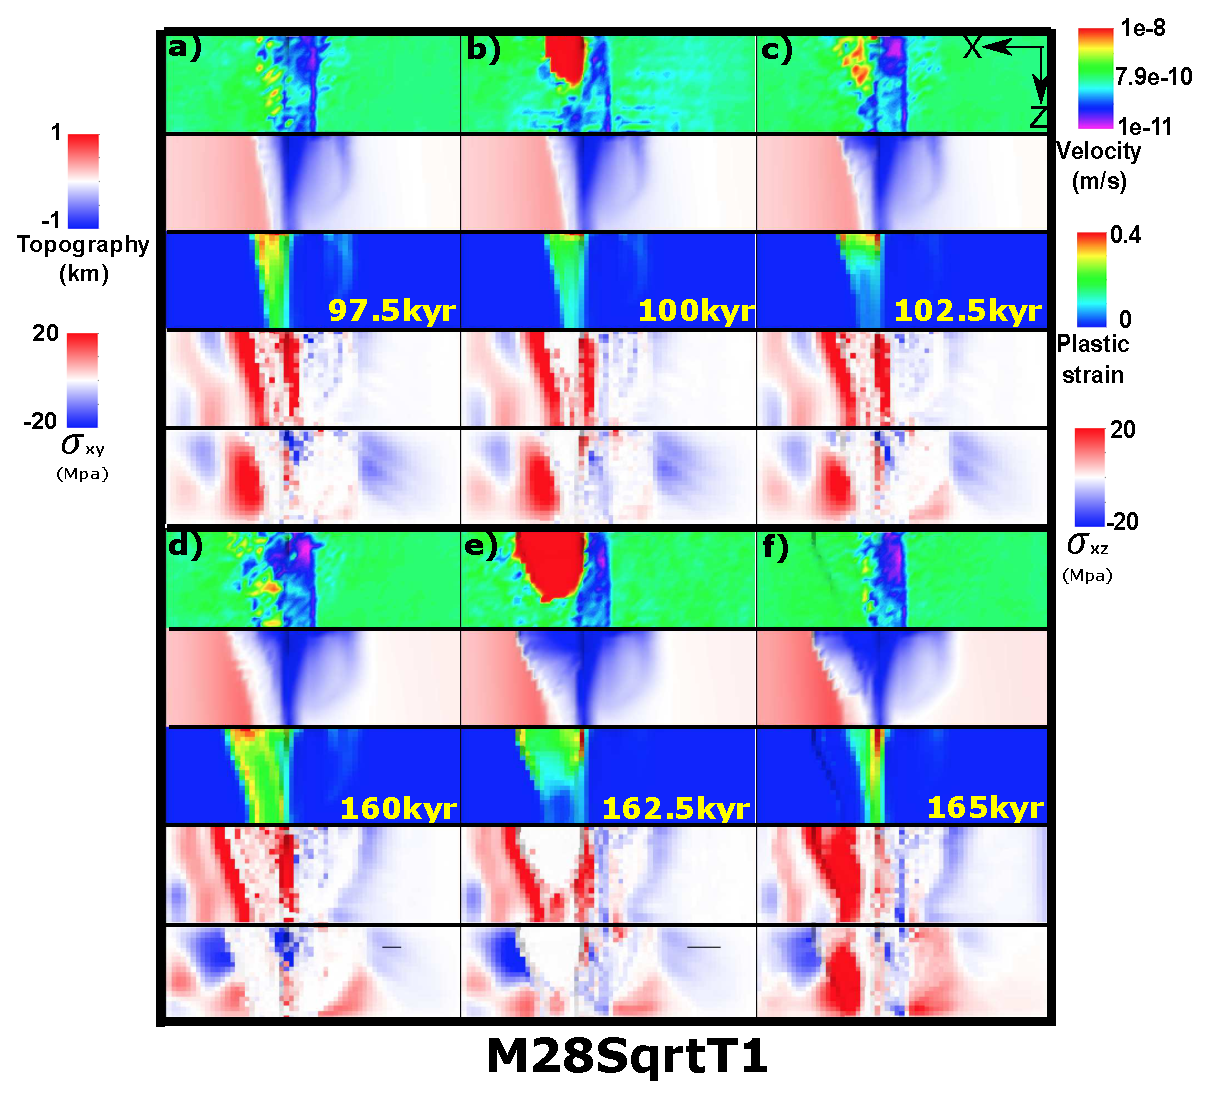
\includegraphics[width=0.8\textwidth]{./Figures/fig_Results4_4_sqrt_cut_back_with_time_1.eps}
  \caption{Plastic strain, topography and stresses evolution for M28SqrtT1.}
 \label{fig_Results4_4}
\end{figure}   

Mass wasting occurs on the exposed surface of a low-angle normal fault. %It happens most frequently in the models with M varying as a squuare root function of along-ridge distance. 
%
%When the tip of the weak fault interface extends with the spreading plate and is intersected by a pre-exisitng shear stress $\sigma_{xy}$ (Figure~\hyperref[fig_Results4_5]{\ref{fig_Results4_5}}), the extra shear stress cuts 
%the tip of the weak fault interface and leads to the decoupling between the spreading plate and the upper layer of the hanging wall of the detachment fault.
%
When a layer of weak fault interface becomes gravitationally unstable and is detached from the underlying material, the detached layer flows towards the ridge axis and the lower M side with a velocity $\sim$10 times faster than the half spreading rate (Figure~\hyperref[fig_Results_3_2_5_Cut-back_velocity]{\ref{fig_Results_3_2_5_Cut-back_velocity}}; Figure~\hyperref[fig_Results4_4]{\ref{fig_Results4_4}.b,e (first row)})). 
%The decoupled upper layer of the hanging wall at the higher M side (0.12 $<$ M $<$ 0.56) flows toward the lower M side with a velocity approximately parallel to the ridge axis (Figure~\hyperref[fig_Results_3_2_5_Cut-back_velocity]{\ref{fig_Results_3_2_5_Cut-back_velocity}}). This is because the topography of the median valley at the higher M side is higher due to a larger amount of magma supply. As the top layer of the footwall flows down the topography slope, obvious topography drop is observed in 2.5 kyr (Figure~\hyperref[fig_Results4_4]{\ref{fig_Results4_4}.b) versus c); d) versus e) (topography)}). 
The mass wasting produces a continuous fault scarp with a relief of $\sim$1 km along the initial breakaway. 
%The total length of the fault scarp extends for about 20 km along the ridge. The distance between the fault scarp and the central dike varies along the ridge (Figure~\hyperref[fig_Results4_4]{\ref{fig_Results4_4}.e (topography)}).  

\begin{figure}[h]
  \centering
    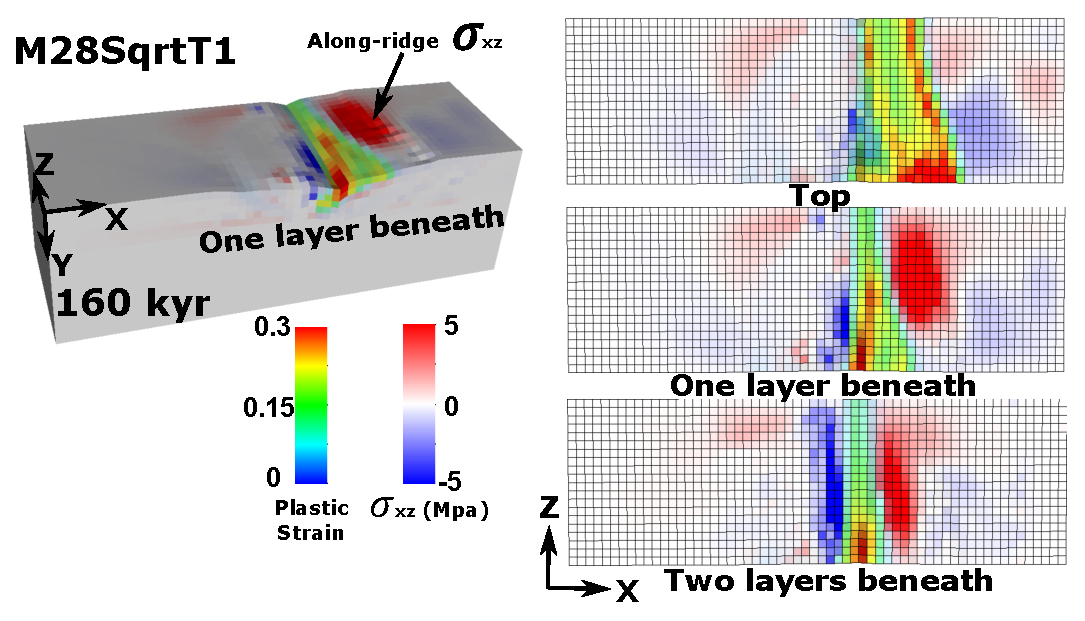
\includegraphics[width=1.0\textwidth]{./Figures/fig_Results_3_2_5_sqrt_cut_back_Sxz_beneath.eps}
  \caption{Along ridge axis $\sigma_{xz}$ (bird's-eye view of three layers of model domain) (positive(red) means clockwise). Plastic strain is plotted with opacity linearly proportional to its value.}
 \label{fig_Results_3_2_5_sqrt_cut_back_Sxz_beneath}
\end{figure}

%Five factors together trigger the cut-back. The unbending force of the bent footwall (Figure~\hyperref[fig_Results4_8]{\ref{fig_Results4_8}}); the pre-existing shear stress that add extra cutting force to the extending tip of the weak detachment fault (Figure~\hyperref[fig_Results4_5]{\ref{fig_Results4_5}}); the shear stress that aligns beneath the detachment fault interface that tends to rotate counterclockwise the hanging wall (viewing into positive $z$-axis direction) (Figure~\hyperref[fig_Results4_5]{\ref{fig_Results4_5}}); the coupling between the conjugate plate and the hanging wall at the lower M side (M $<$ 0.5) that pulls the hanging wall toward the ridge axis; and the asynchronous fault inistiation as well as the along ridge variation in the rate of fault slip due to varying M that tend to syncrhonize the faulting along the ridge and resists the faster extension of the termination at the higher M side (Figure~\hyperref[fig_Results_3_2_5_sqrt_cut_back_Sxz_beneath]{\ref{fig_Results_3_2_5_sqrt_cut_back_Sxz_beneath}}).

%As shown in Figure~\hyperref[fig_Results4_8]{\ref{fig_Results4_8}}, due to bending of the crust at the footwall side, below the blue neutral plane, $\sigma_{xx}>0$, meaning tensional stress increases as fault slips. The resulting force tends to unbend the bent crust and drag down the connecting surface (the future decoupled hanging wall).

\begin{figure}[h]
  \centering
    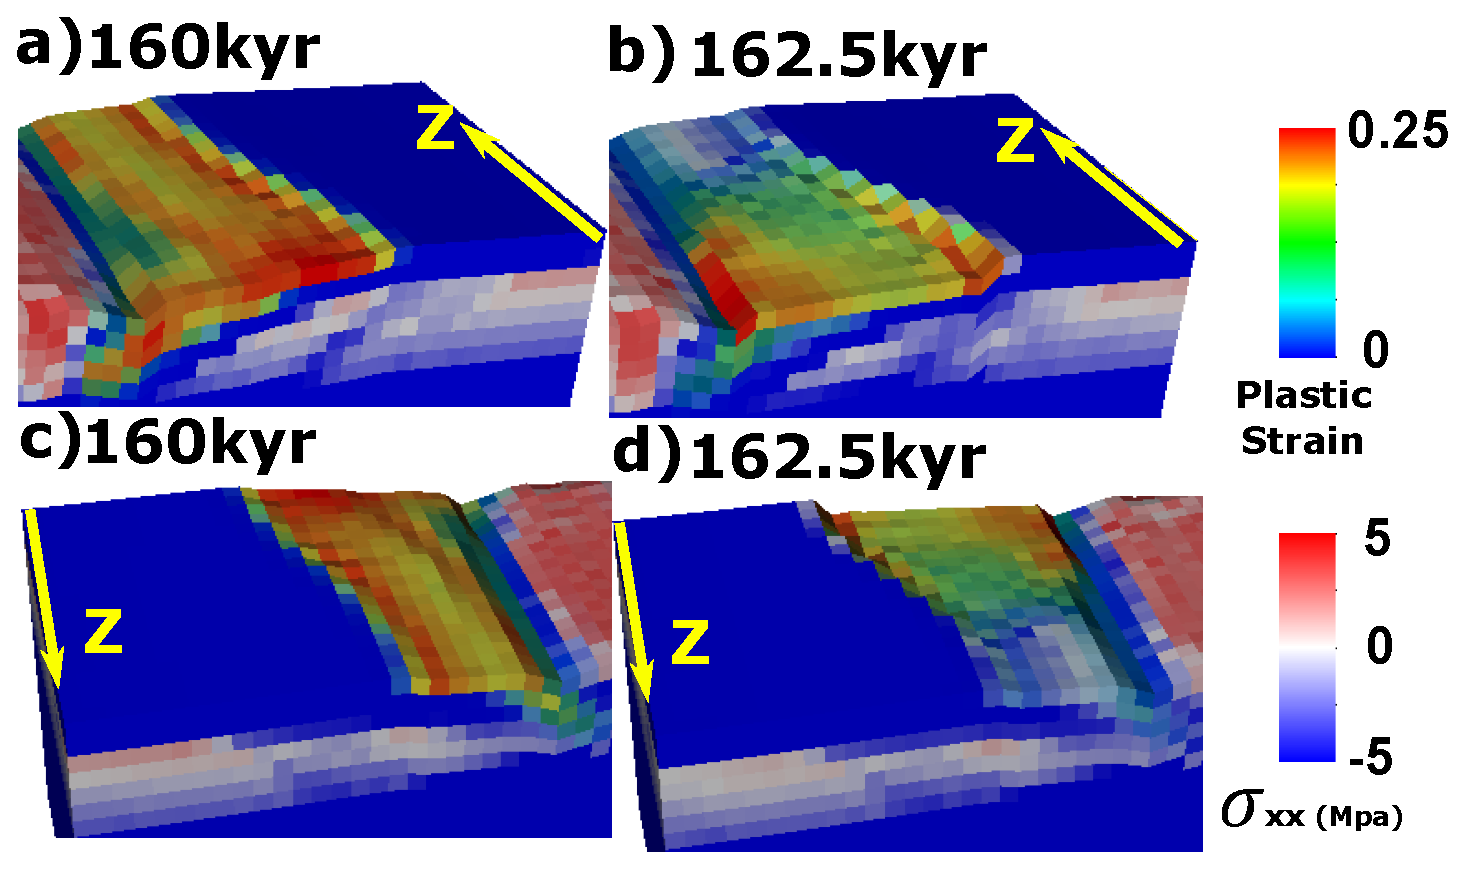
\includegraphics[width=0.6\textwidth]{./Figures/fig_Results4_6_sqrt_cut_back_bending_drop.eps}
  \caption{M28SqrtT1 (Table~\hyperref[Tab1_1]{\ref{Tab1_1}}). Bending stress drop (a versus b) at the lower M side due to the cut-back. No bending stress drop (c versus d) at the higher M side as a comparison.}
 \label{fig_Results4_6}
\end{figure}

%Mass wasting only happens at the lower M side as indicated by the red-colored (i.e., high-speed) block (``a large slump block'' \citep{Smith2014}) of Figure~\hyperref[fig_Results4_4]{\ref{fig_Results4_4}.b,e (velocity)}. The tensional stress due to bending is released at the lower M side (0.2 $<$ M $<$ 0.57) (Figure~\hyperref[fig_Results4_6]{\ref{fig_Results4_6}.a compared to b}), however, the cut-back does not propogates to the higher M side and the tensional bending stress is not released (Figure~\hyperref[fig_Results4_6]{\ref{fig_Results4_6}.c compared to d}). This difference in the bending stresses between the lower and higher M sides is partly due to the decouple between lower and higher M side hanging walls. In addition, once the cut back happens at 162.5 kyr, the $\sigma_{xy}$, $\sigma_{xz}$ and $\sigma_{xx}$ are released (Figure~\hyperref[fig_Results4_4]{\ref{fig_Results4_4}.e (fourth and fifth row: $\sigma_{xy}$ and $\sigma_{xz}$)}). %After the cut back, the termination of the detachment fault recedes backwards for about 7 km towards the ridge axis (Figure~\hyperref[fig_Results4_4]{\ref{fig_Results4_4}.f (third row: plastic strain)}).% (termination fronts are always consistent with tension stresses in $\sigma_{xx}$ and $\sigma_{zz}$ as well as with plastic strain front(due to healing, high plastic strain region corresponds only to region with continuously deformation) (Figure~\hyperref[fig_Results4_3_1]{\ref{fig_Results4_3_1}} and Figure~\hyperref[fig_Results4_3_2]{\ref{fig_Results4_3_2}})).
% because $\sigma_{xy}$ always accummulates immediately beneath the normal fault interface. The red $\sigma_{xz}$ on the positive $x$-axis direction of the new termination is due to the along ridge axis variatioin in the rate of fault slip.  

\begin{figure}[h]
  \centering
    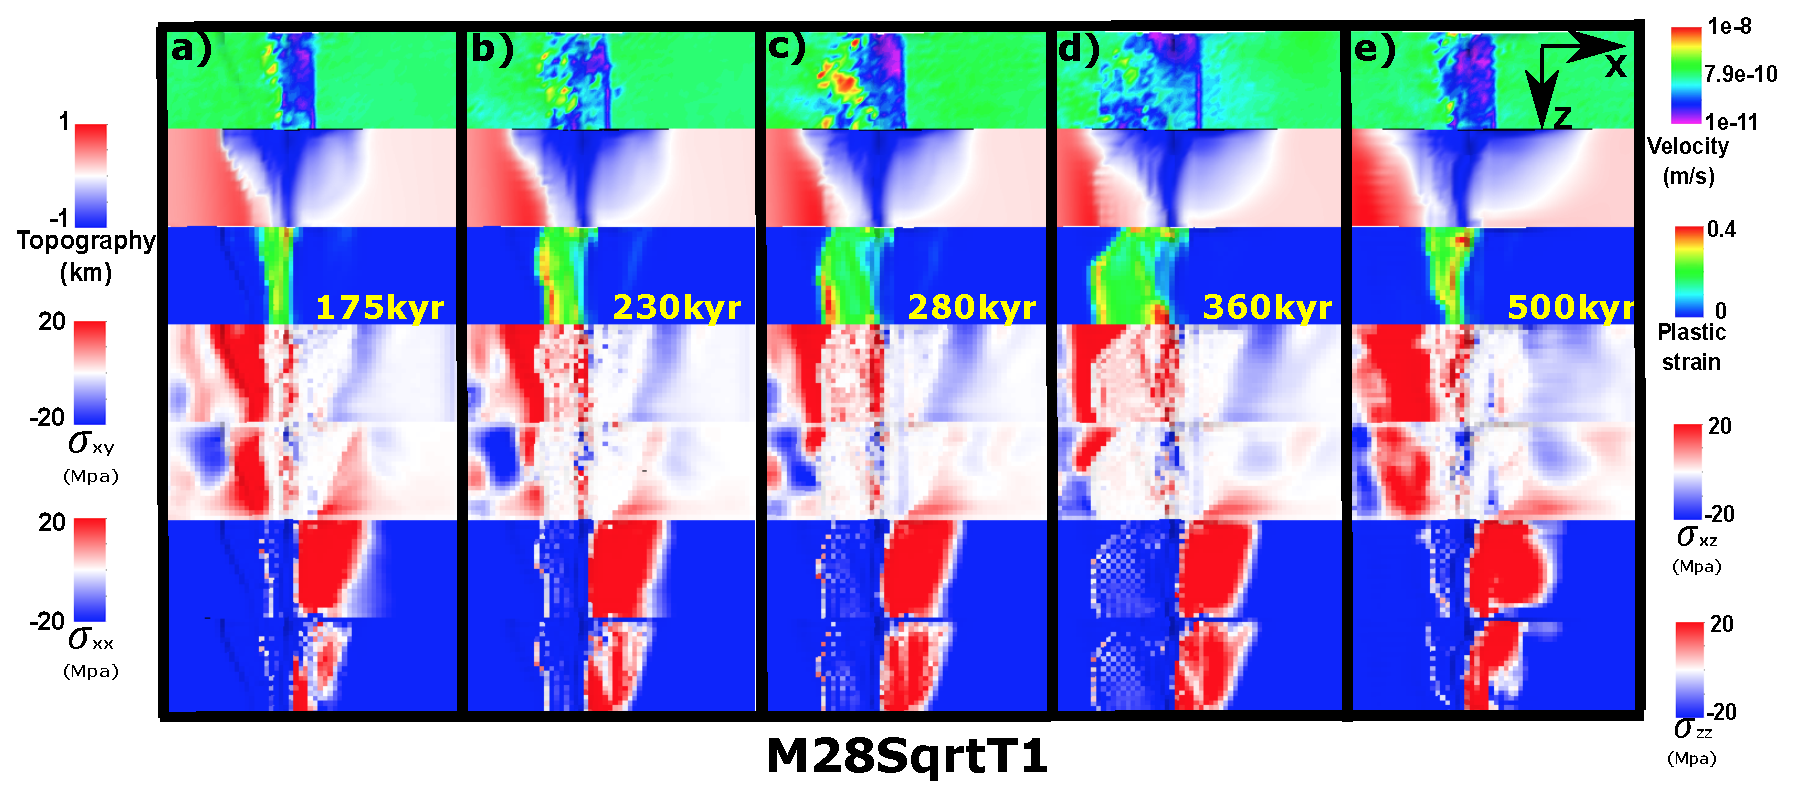
\includegraphics[width=1.0\textwidth]{./Figures/fig_Results4_9_sqrt_cut_back_new_fault_chase.eps}
  \caption{New fault front chase after cut-back.}
 \label{fig_Results4_9}
\end{figure}

Immediately after an event of mass wasting, the fault trace jumps towards the ridge axis (Figure~\hyperref[fig_Results4_4]{\ref{fig_Results4_4}.d versus f (third row: plastic strain)}). 
%This behavior helps maintain a high angle normal fault. 
Then, $\sigma_{xy}$ and $\sigma_{xz}$ soon \annote[EC]{fill in the area}{What do you mean by ``stresses filling an area''?} between cut-back created fault scarp and the new termination (Figure~\hyperref[fig_Results4_4]{\ref{fig_Results4_4}.f (fourth and fifth row: $\sigma_{xy}$ and $\sigma_{xz}$)}. \note[EC]{don't understand the rest of this paragraph.}
After that, the termination at the higher M side extends faster and further than the lower M side (Figure~\hyperref[fig_Results4_9]{\ref{fig_Results4_9}.a$\sim$d}). This is because during the cut-back, tensional stress due to bending is released at the lower M side but continues to accummulate at the higher M side. At the lower M side, it needs time to reach the previous tensional stress state and then starts from there to pull the new termination away from the ridge axis. While at the higher M side the increasing tensional stress directly leads to a fast extending termination.
%\add[XT]{One question is, how to explain that the fault front is moving much faster than the initial abandoned breakaway? New fault front soon reach the old breakaway.}

This phenomenon is responsible for the corrugations observed. It creates an ``X'' shape ``scan'' that first ``scan'' the topography with the faster low M side (Figure~\hyperref[fig_Results4_4]{\ref{fig_Results4_4}.d and e}) and then ``scan'' with the faster higher M side (Figure~\hyperref[fig_Results4_9]{\ref{fig_Results4_9}.c and d}). This results in a evolving curved termination that produces mullion structures (Figure~\hyperref[fig_Results4_9]{\ref{fig_Results4_9}.d}). \note[EC]{Can't follow what you say.}  

\subsubsection{Hourglass-shaped median valley}

\begin{figure}[h]
  \centering
    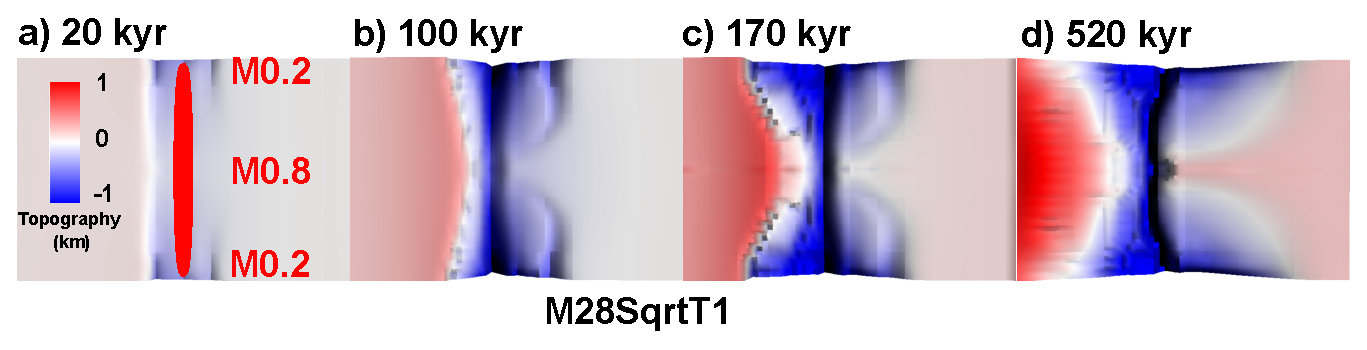
\includegraphics[width=1.0\textwidth]{./Figures/fig_Results_3_2_hourglass_evolution.eps}
  \caption{Bird's-eye view of the evolution of the hourglass shape median valley. It is generated by attaching the topography of the M28SqrtT1 model to its mirror reflection by assumming symmetrical M variation (0.2 to 0.8 to 0.2). }
 \label{fig_Results_3_2_hourglass_evolution}
\end{figure}

A median valley takes a hourglass shape whenever M varies along the ridge. The hourglass shapes vary with time and the functional form of M variation. %As shown in Figure~\hyperref[fig_Results_3_2_hourglass_evolution]{\ref{fig_Results_3_2_hourglass_evolution}.a}, initially, 
A median valley initially has similar width along the ridge but is deeper on the lower M side where normal faults first form. By $\sim$100 kyr (Figure~\hyperref[fig_Results_3_2_hourglass_evolution]{\ref{fig_Results_3_2_hourglass_evolution}.b}), the fault on the negative $x$-axis direction of the ridge axis doesn't propagates to the higher M side of the ridge and becomes inactive. It produces a depressed topography curve following the inactive fault trace, which is further away from the ridge axis at the lower M side but closer to ridge axis at the higher M side. On the other side of the ridge axis, as the active fault rotates to a lower dip angle, it generates breakaways that are further away from the ridge axis at the lower M side while closer to the ridge axis at the higher M side. This along ridge variation in the location of the breakaways act as another boundary of the hourglass. Both boundaries are extended following the spreading plates. By $\sim$170 kyr (Figure~\hyperref[fig_Results_3_2_hourglass_evolution]{\ref{fig_Results_3_2_hourglass_evolution}.c}), the hourglass become wider and deeper. Since the area of the cross-section along the ridge inside the hourglass shape median valley is approximately inversely proportional to the local M values, the shape of the hourglass varies with different M variations.

\begin{figure}[h]
  \centering
    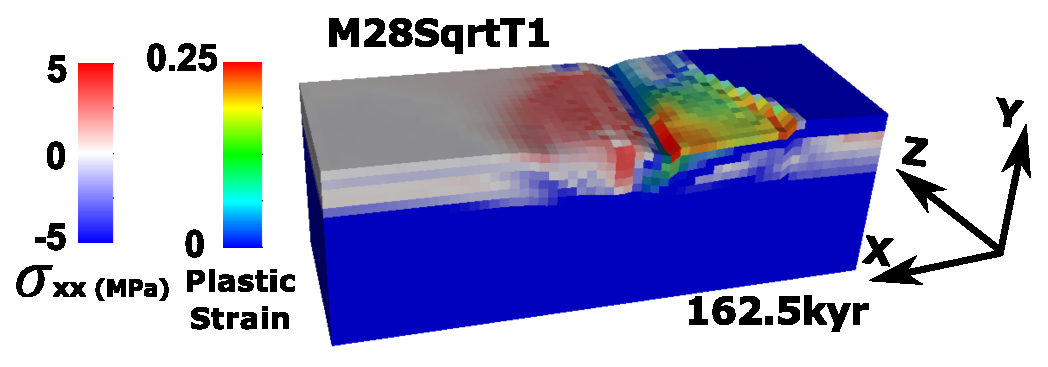
\includegraphics[width=0.6\textwidth]{./Figures/fig_Results4_7_sqrt_cut_back_conjugate_Sxx.eps}
  \caption{Higher $\sigma_{xx}$ shows inside the median valley on the negative $x$-axis direction of the ridge axis. }
 \label{fig_Results4_7}
\end{figure}

The further depression inside the median valley is mostly due to the elastic deformation from crustal extension. As shown in Figure~\hyperref[fig_Results4_7]{\ref{fig_Results4_7}}, the $\sigma_{xx}$ in the median valley is higher because that the brittle crust is the thinnest at the median valley, when same amount of force propagates from far field extension to the median valley, the stress increases. This increased $\sigma_{xx}$ is responsible for the further depression and extension of the median valley on the negative $x$-axis direction of the ridge axis (Figure~\hyperref[fig_Results_3_2_hourglass_evolution]{\ref{fig_Results_3_2_hourglass_evolution}.d}). For the median valley on the other side of the ridge axis, cut-back triggered mass wasting between the breakaways and the ridge axis results in the further lowering in topography (Figure~\hyperref[fig_Results4_4]{\ref{fig_Results4_4}.d versus e (topography)}). 

\subsubsection{Corrugations and mullion structures}

Both corrugations and mullion structures are linear structures parallel to the spreading direction. As shown in Figure~\hyperref[fig_Results1_1]{\ref{fig_Results1_1}.f}, at the M $<$ 0.5 area on top of the OCC surface, corrugations show a uniform wavelength of $\sim$1 km with hundreds meters in amplitude. While at the higher M side of the ridge (Figure~\hyperref[fig_Results1_1]{\ref{fig_Results1_1}.g}), a mullion structure of a wavelength of $\sim$7 km. In spite of morphological similarity, corrugations and mullion structures have different formation mechanisms. 

\paragraph{Corrugations}

\begin{figure}[h]
  \centering
    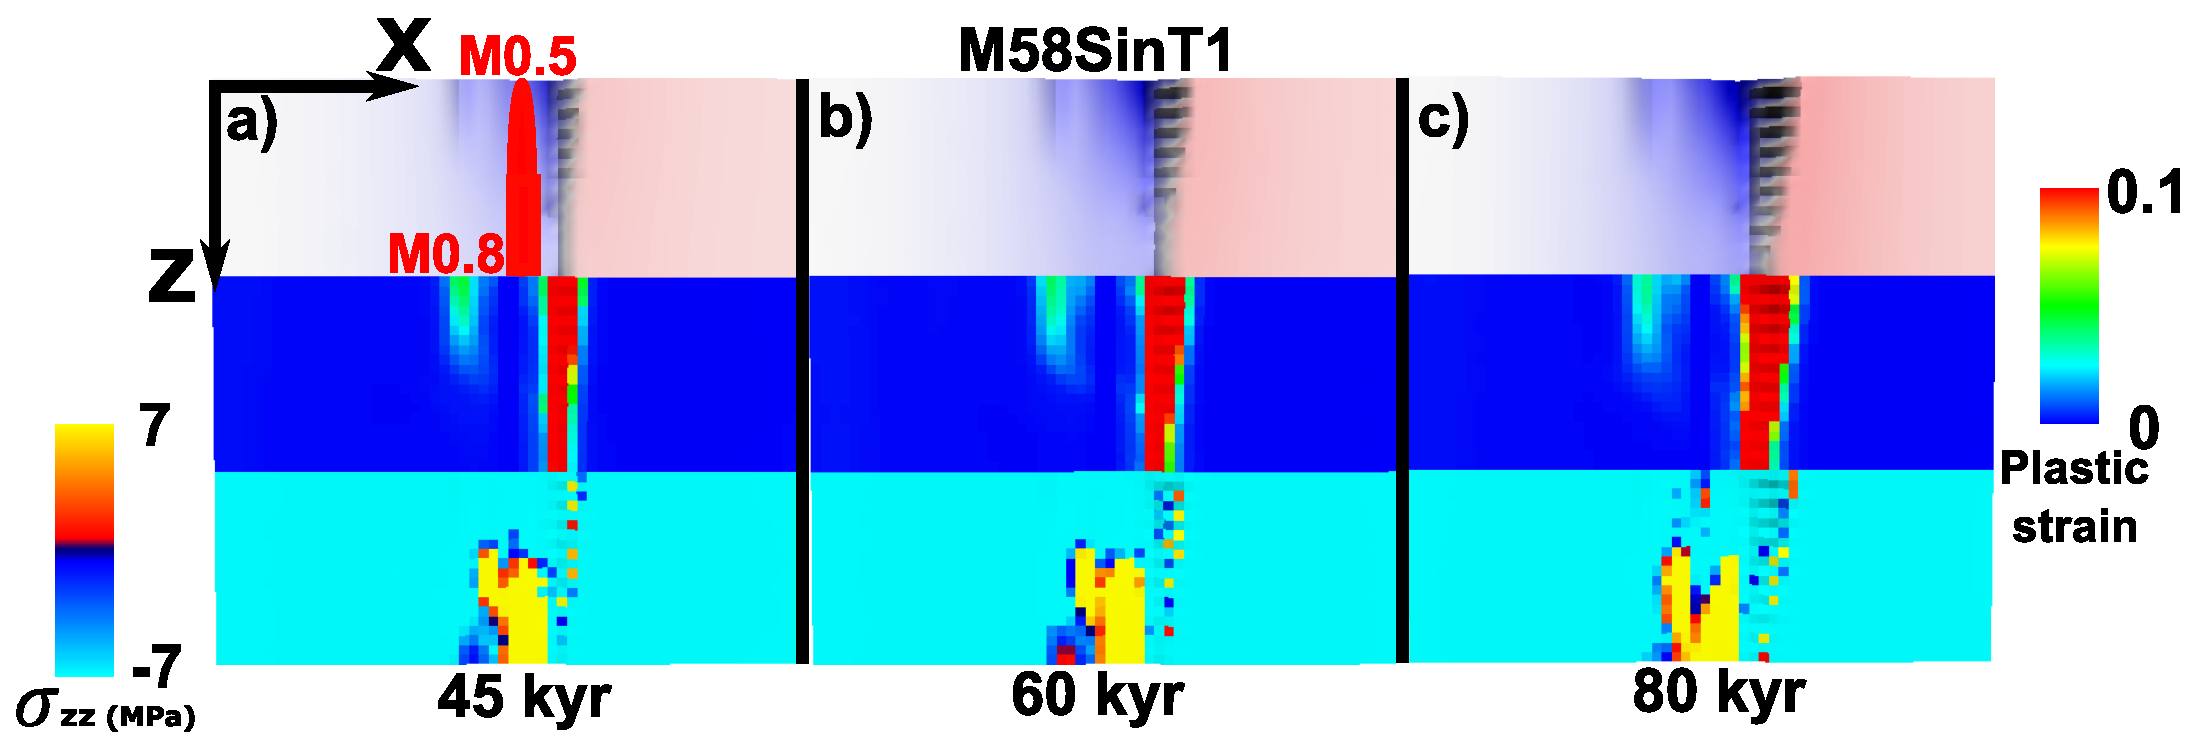
\includegraphics[width=1.0\textwidth]{./Figures/fig_Results_3_2_6_corrugations_evolution.eps}
  \caption{Bird's-eye view of the evolution of the corrugations. Color scales for the topography is the same as Figure~\hyperref[fig_Results1_1]{\ref{fig_Results1_1}}.}
 \label{fig_Results_3_2_6_corrugations_evolution}
\end{figure}

~\\

\paragraph{Corrugations}

The corrugation is produced at the front tip of the \annote[EC]{extending}{What do you mean by ``extending'' plastic strain?} plastic strain by tensile failure in the along-$z$-axis direction. As shown in Figure~\hyperref[fig_Results_3_2_6_corrugations_evolution]{\ref{fig_Results_3_2_6_corrugations_evolution}}, when the plastic strain reaches or excedes 0.1 (red color), base on type 1 weakening, the cohesion decreases to 4 Mpa. With a 30 $\degree$ friction angle, tensile failure is declared when the $\sigma_{zz}$ reaches $\sim$7 Mpa (yellow color).
The tensile stress is due to the asynchronous faulting along the ridge. Faulting initiates earlier at the lower M side of the ridge. As the fault offsets more on the low M side than on the high M side, the footwall of the fault rotates and get uplifted more on the low M side. The footwalls along the ridge generates the isochron-parallel tesional stress $\sigma_{zz}$. Since $\sigma_{zz}$ follows along the extending tip of the plastic strain and as \annote[EC]{the extending tip of the plastic strain extends}{What do you mean?}, $\sigma_{zz}$ also \annote[EC]{extends}{What do you mean by a stess component ``extends''?}. Extending tip of the plastic srain together with $\sigma_{zz}$ generate tensile failure that extends away from the ridge axis and thus produces the linear corrugations that are parallel to the spreading velocity. Detail analysis along with simpler model experiments are given in the ``Discussion'' section.   

\note[EC]{These sentences would better fit in model comparison section or Discussion.}
Corrugations are observed in most of the models except for the constant M model M88ContT2 (Figure~\hyperref[fig_Results1_3]{\ref{fig_Results1_3}}). Among the models that have corrugations, the timing, location and the regularity of the corrugations varies. For example, corrugations in M58SinT1 shows up $\sim$45 kyr at the lower M side (0.5 $<$ M $<$ 0.65) (Figure~\hyperref[fig_Results_3_2_6_corrugations_evolution]{\ref{fig_Results_3_2_6_corrugations_evolution}.a)}). However, corrugations in M28LinT1 shows up much later at $\sim$240 kyr at the lower M side (0.2 $<$ M $<$ 0.38) (Figure~\hyperref[fig_Results1_1]{\ref{fig_Results1_1}.c}). For M28LinT1, the corrugations are mostly formed at the lower M side (M $<$ 0.5) through time and they are less regular along the ridge ((Figure~\hyperref[fig_Results1_1]{\ref{fig_Results1_1}.h})). But the corrugations in M58SinT1 appear along the whole ridge and shows regularly alternative undulations with a wavelength of $\sim$1 km (Figure~\hyperref[fig_Results_3_2_6_corrugations_evolution]{\ref{fig_Results_3_2_6_corrugations_evolution}.c)}). 


\paragraph{Mullion structures}

\begin{figure}[h]
  \centering
    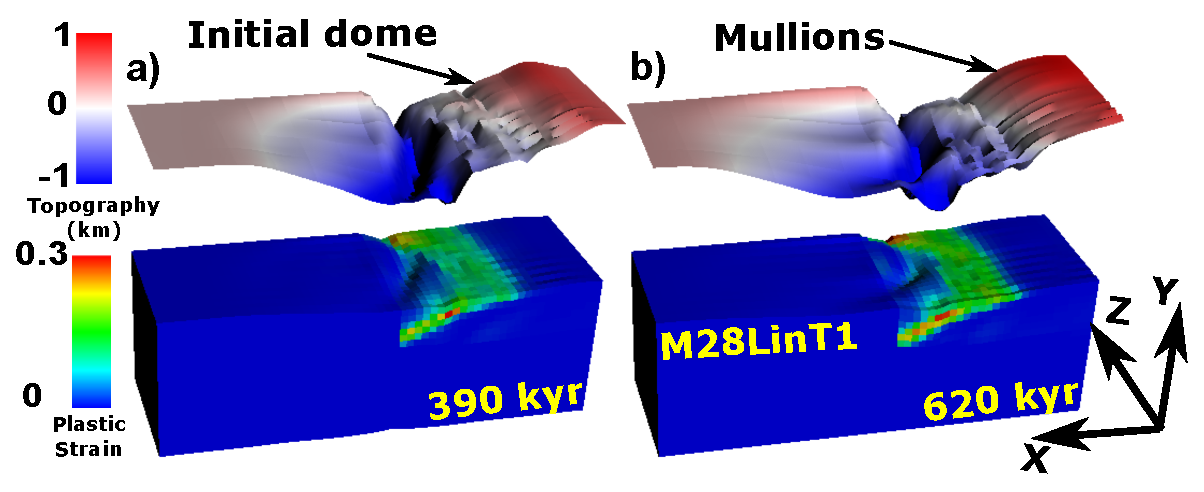
\includegraphics[width=1.0\textwidth]{./Figures/fig_Results_3_2_6_mullion_evolution.eps}
  \caption{Evolution of mullion structures.}
 \label{fig_Results_3_2_6_mullion_evolution}
\end{figure}
~\\
Mullion structures observed in the models are formed by the along ridge variation in the location of the termination due to the evolution of faulting. They usually appear at where the termination is closer to the ridge axis. The shape of the footwall follows the trace of the termination as it is exhumed to the surface. At where the termination is bent inward to the ridge axis, an ``initial dome'' (Figure~\hyperref[fig_Results_3_2_6_mullion_evolution]{\ref{fig_Results_3_2_6_mullion_evolution}.a)}) is produced once the hanging wall is exhumed to the seafloor. The wavelength of the mullion structure is determined by the shape of the termination. If the pattern of the termination lasts for a long time and the footwall of the detachment fault keeps being exhumed to the surface following the trace of the detachment fault termination, a mullion structure is produced (Figure~\hyperref[fig_Results_3_2_6_mullion_evolution]{\ref{fig_Results_3_2_6_mullion_evolution}.b)}). 


\subsection{Effects of the functional forms of M variation}

\subsubsection{M28(Lin, Sin, Sqrt)T1}

Comparing M28LinT1, M28SinT1 and M28SqrtT1, major differences lie in the model behaviors of the ``inward fault jump'', the ``cut-back'' and the ``hourglass shape median valley''. All three models have no fault alternation.    

\begin{figure}[h]
  \centering
    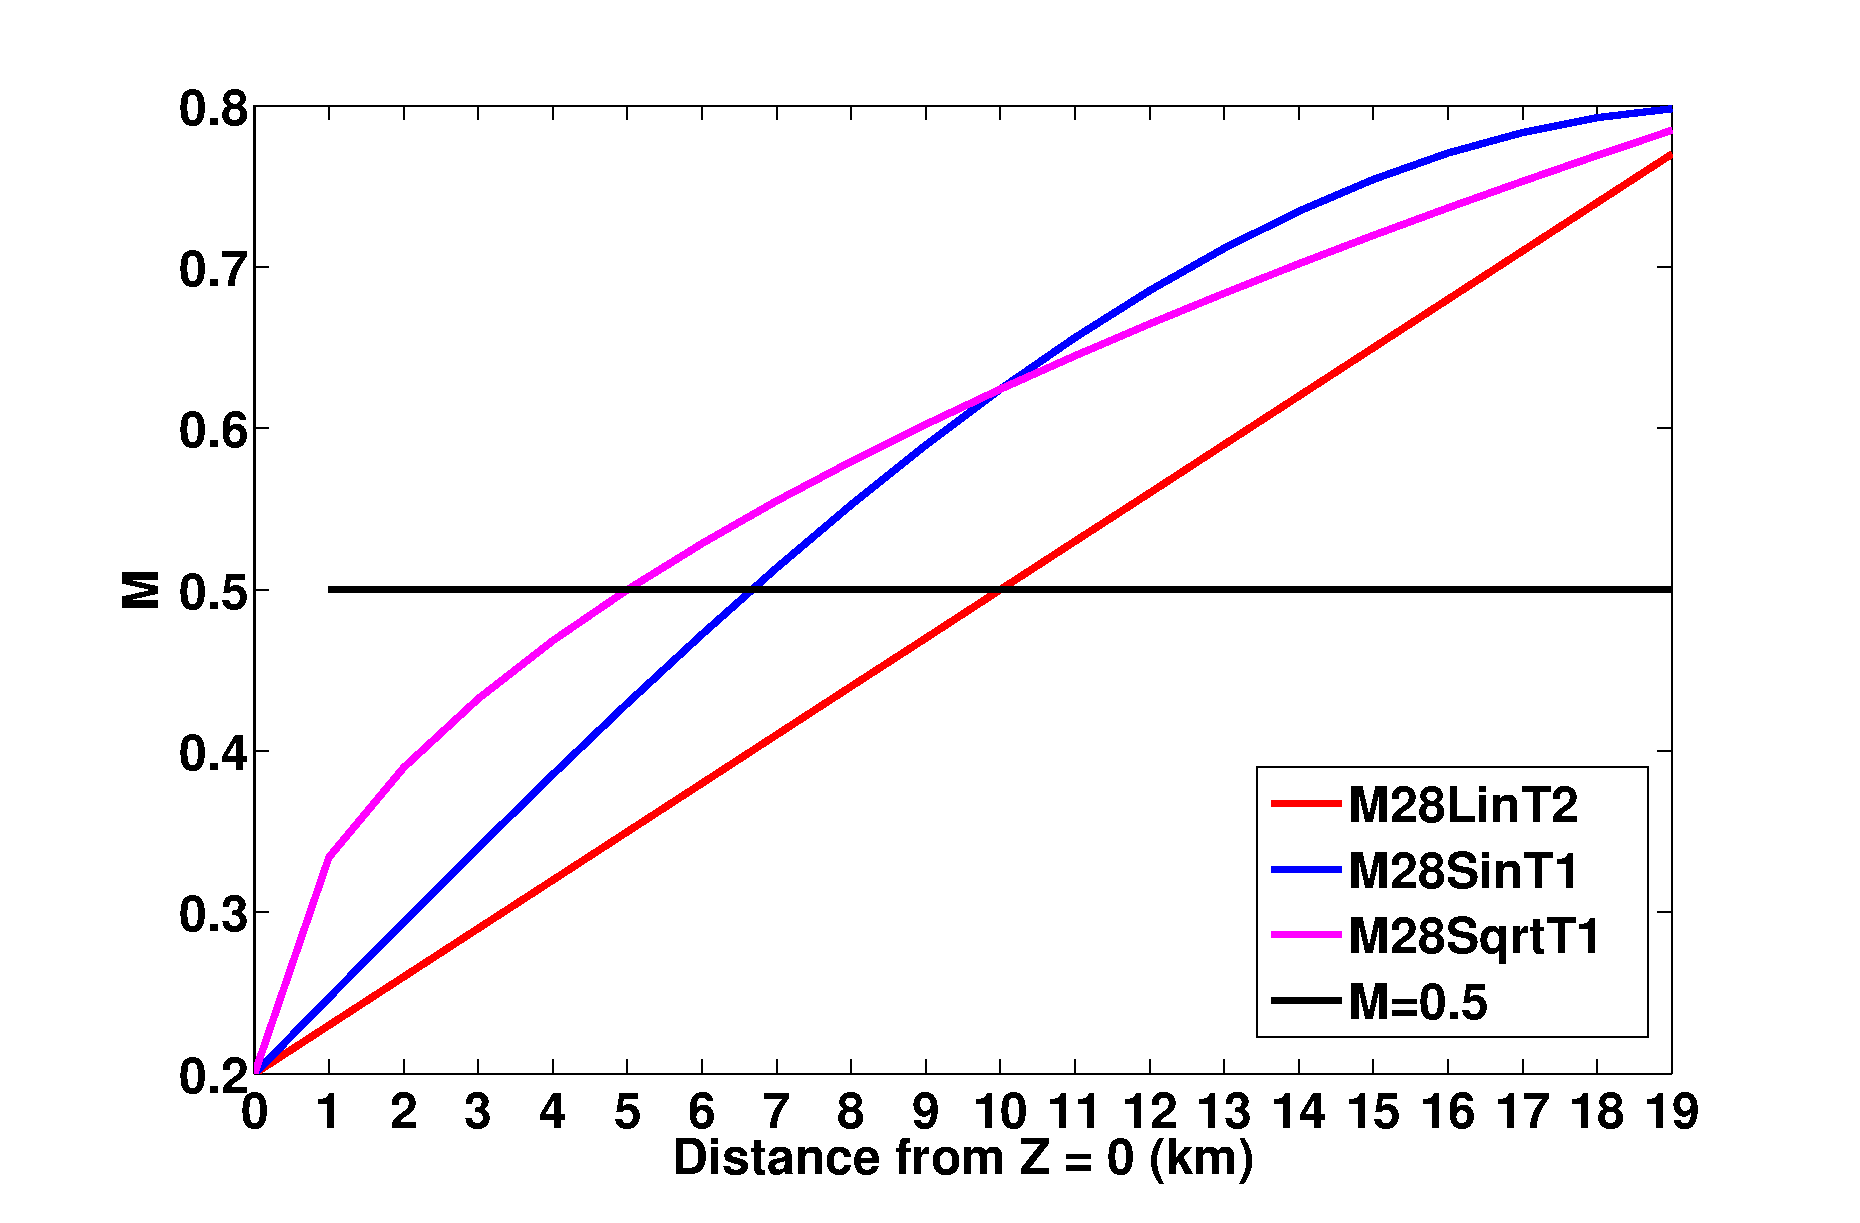
\includegraphics[width=0.8\textwidth]{./Figures/fig_Results_3_3_M_variation.eps}
  \caption{Three functional forms of M variation. M begins to exceed the M $=$ 0.5 black line at Z=10 km, 7 km, 5 km for M28LinT1, M28SinT1 and M28SqrtT1 respectively.}
 \label{fig_Results3_1}
\end{figure}   

\paragraph{Inward fault jump}\label{para_InwardFaultJump}
~\\
Only linear and sinusoidal models have inward fault jump. Sqaure root model shows no inward fault jump because during cut-back, termination of the detachment fault retreats backward toward the ridge axis and the detachment fault is maintained near the ridge axis.

Between linear and sinusoidal models, timing and dimension of the inward jumping faults are different. For the linear functional form, the inward fault jump at the higher M side starts accommodating most of the extension at $\sim$900 kyr and replaces the initial detachment fault (Figure~\hyperref[fig_Results4_2]{\ref{fig_Results4_2}}, Figure~\hyperref[fig_Results1_1]{\ref{fig_Results1_1}.f}). It nucleates from the ridge center where M $=$ 0.5 and then propagates to the M $=$ 0.8 end with a length of $\sim$11 km. 
 %This secondary fault creates another dome with initial composition likely to be volcanic rather than ultramafic, however, as it evolves, if it can last long enough to cut through the whole crust, mantle materials might exhume to the surface. The composition of the domes observed at Kane magamullions is similar to this mechanism between ultramafic babel dome and eastern to it the crustal inside-corner high.  its spatial distribution is at M$>0.5$ region.
For the sinusoidal functional form, the inward fault jump takes the place of the initial detachment fault earlier at $\sim$550 kyr with a length of $\sim$14 km (Figure~\hyperref[fig_Results4_2]{\ref{fig_Results4_2}}).

\begin{figure}[h]
  \centering
    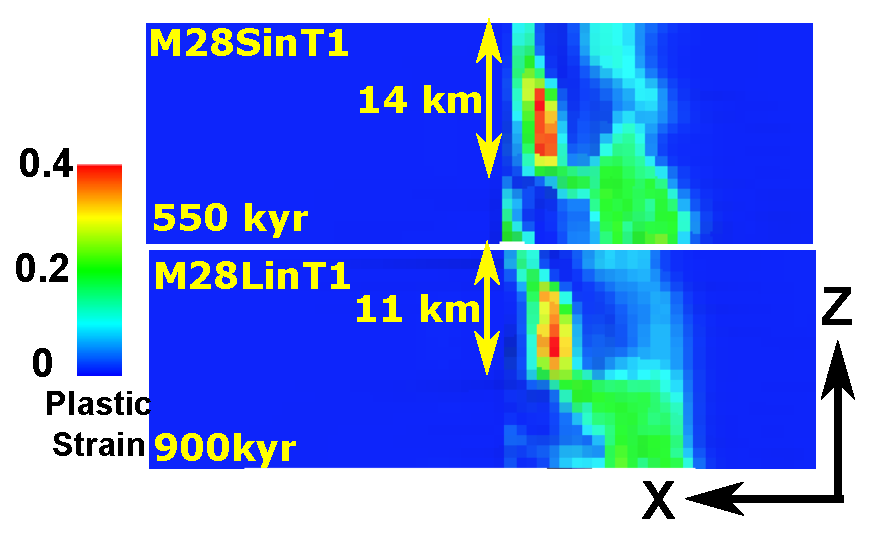
\includegraphics[width=0.6\textwidth]{./Figures/fig_Results4_2_secondary_fault_length_comparison1.eps}
  \caption{Bird's-eye view for comparing the length and timing of inward fault jump.}
 \label{fig_Results4_2}
\end{figure}   

The timing difference between the linear and sinusoidal models is because M28SinT1 consistently has a higher M values than the M28LinT1 (Figure~\hyperref[fig_Results3_1]{\ref{fig_Results3_1}}), which results in that the initial detachment fault at the higher M side (M $>$ 0.5) of M28SinT1 is pushed off axis faster than M28LinT1 and thus forming an earlier inward fault jump. The length difference is because M28SinT1 has a greater length along the ridge axis of M $\ge$ 0.5 (Figure~\hyperref[fig_Results3_1]{\ref{fig_Results3_1}}). 

\paragraph{Cut-back}

\begin{figure}[h]
  \centering
    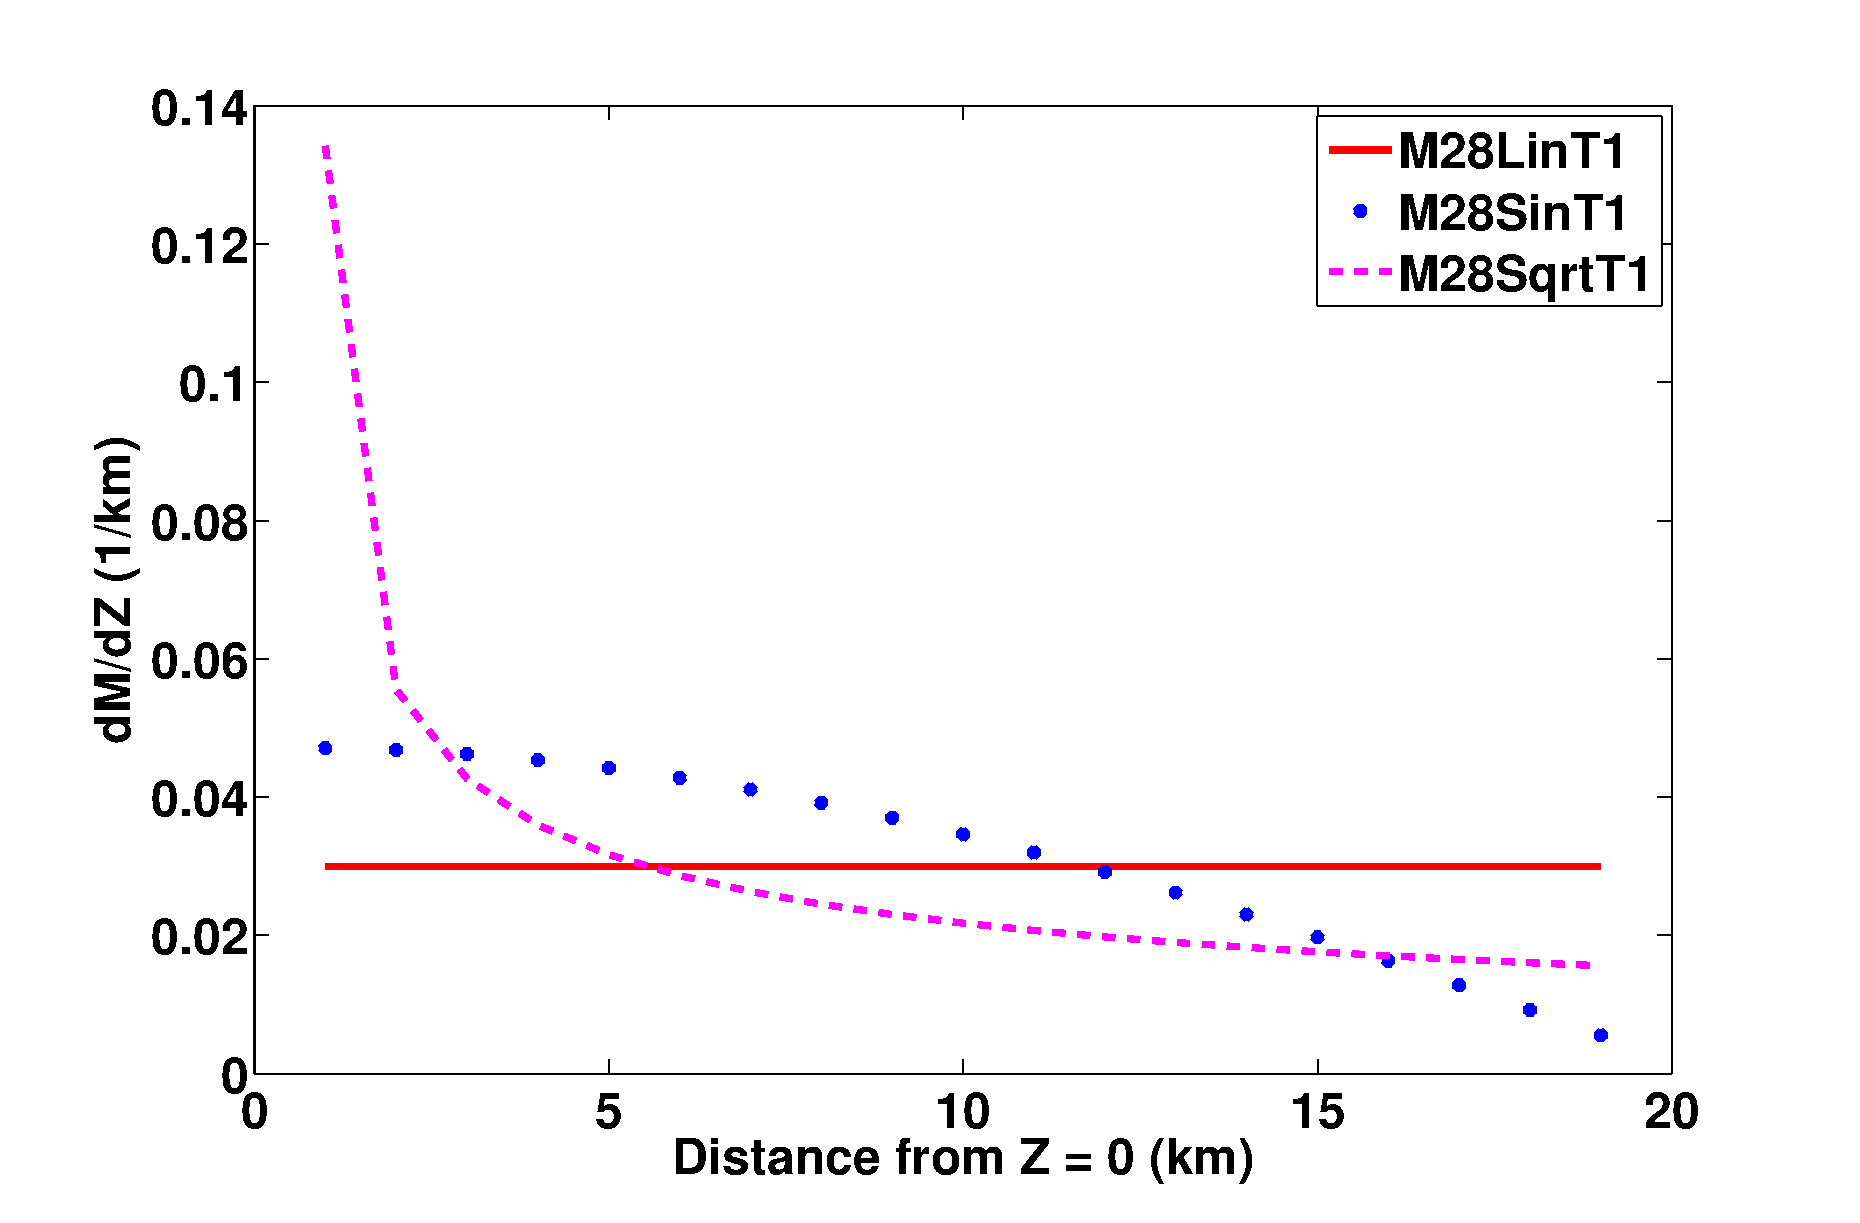
\includegraphics[width=0.8\textwidth]{./Figures/fig_Results_3_3_1_M_type_plot_dM_dZ.eps}
  \caption{$\partial M/ \partial Z$ comparision.}
 \label{fig_Results_3_3_1_M_type_plot_dM_dZ}
\end{figure}  

~\\
Cut-back only happens in the M28SqrtT1 model. Qualitatively, it is because M28Sqrt has a much higher value of $\frac{\partial M}{\partial Z}$ at the lower M side (Figure~\hyperref[fig_Results_3_3_1_M_type_plot_dM_dZ]{\ref{fig_Results_3_3_1_M_type_plot_dM_dZ}}), which implies a larger along ridge shear stress $\sigma_{xz}$ as well as a larger difference in $\sigma_{xy}$ along the ridge that result in the decoupling between the higher and lower M sides hanging walls. 

\iffalse
\begin{figure}[h]
  \centering
    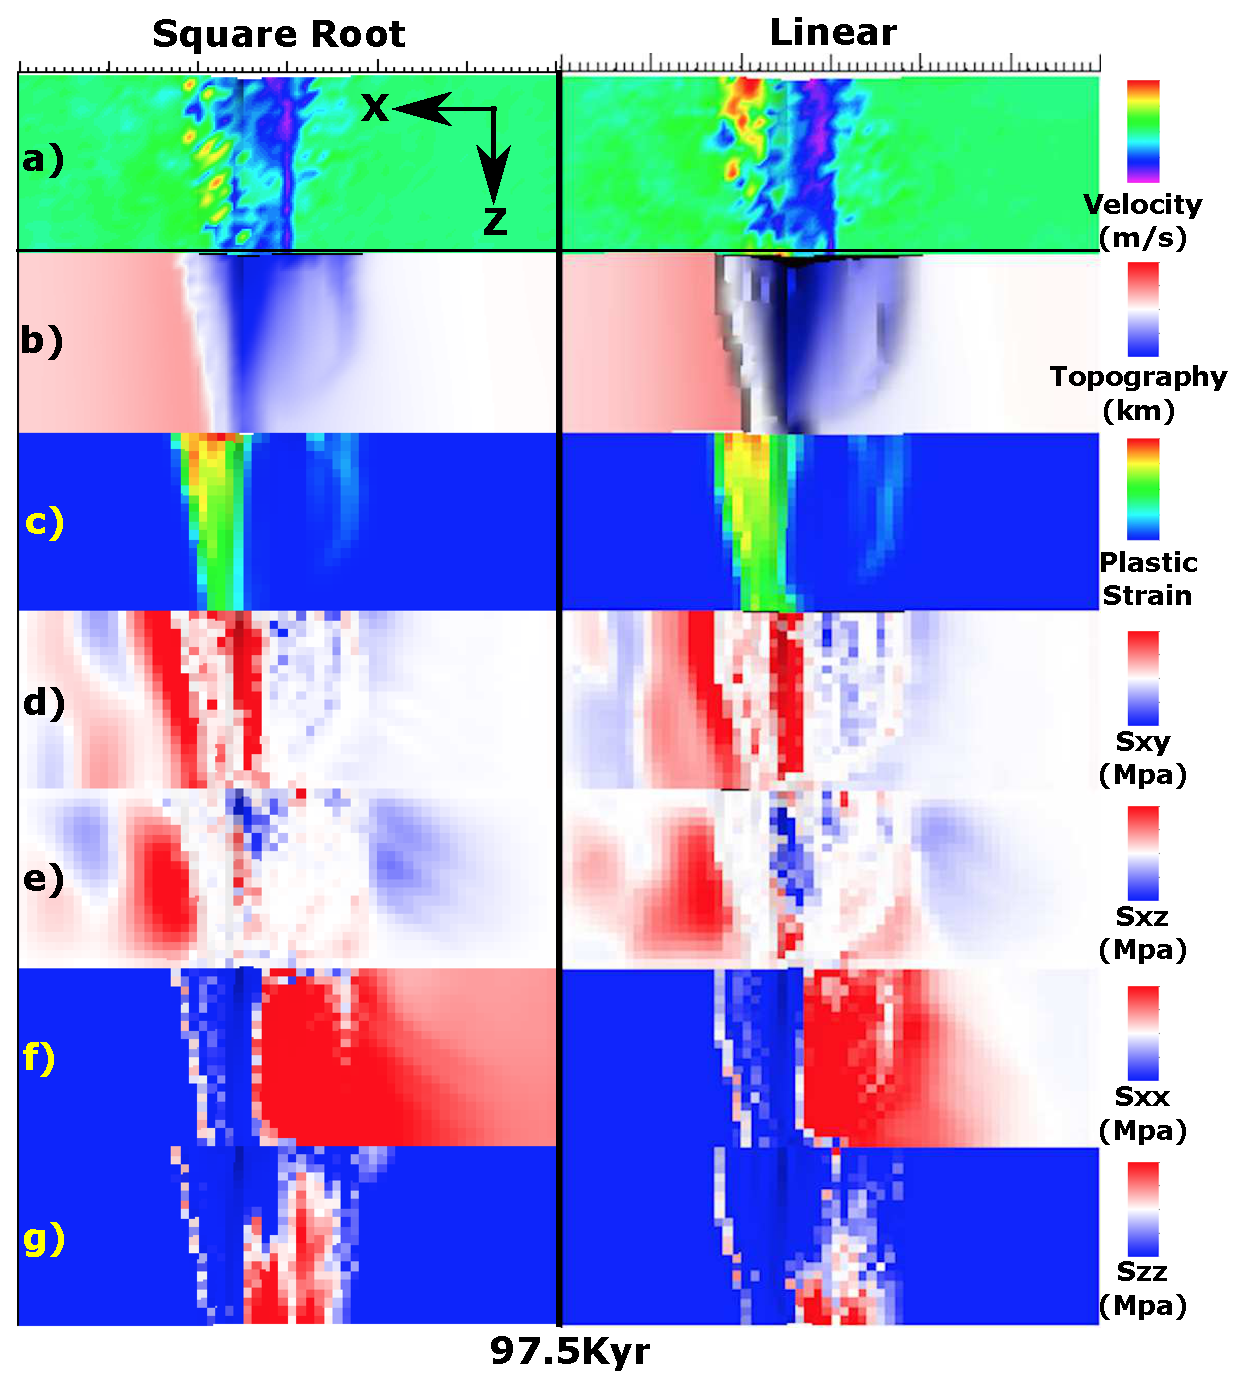
\includegraphics[width=0.6\textwidth]{./Figures/fig_Results4_3_sqrt_vs_lin_cut_back_97kyr.eps}
  \caption{M28LinT1 versus M28SqrtT1 (Table~\hyperref[Tab1_1]{\ref{Tab1_1}}) at 97 kyr. View from top of the model.}
 \label{fig_Results4_3_1}
\end{figure}  

\begin{figure}[h]
  \centering
    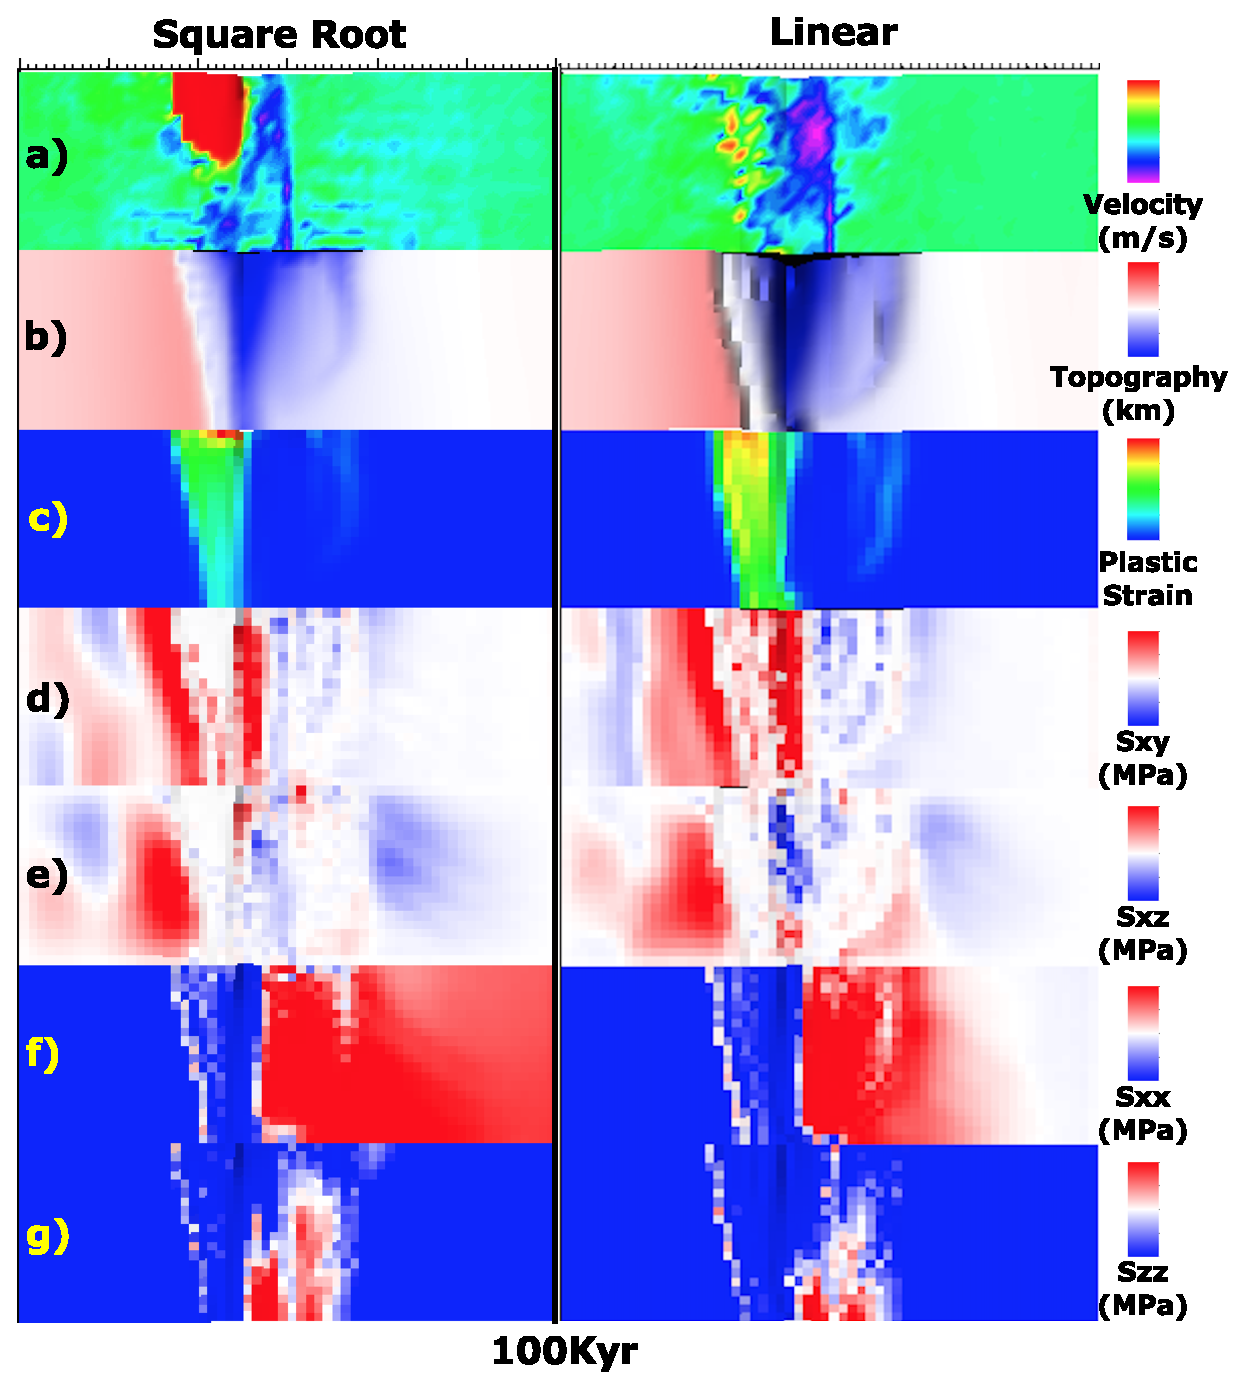
\includegraphics[width=0.6\textwidth]{./Figures/fig_Results4_3_sqrt_vs_lin_cut_back_100kyr.eps}
  \caption{M28LinT1 versus M28SqrtT1 (Table~\hyperref[Tab1_1]{\ref{Tab1_1}}) at 100 kyr. View from top of the model.}
 \label{fig_Results4_3_2}
\end{figure} 
\fi

\paragraph{Hourglass shape median valley}
~\\
\begin{figure}[h]
  \centering
    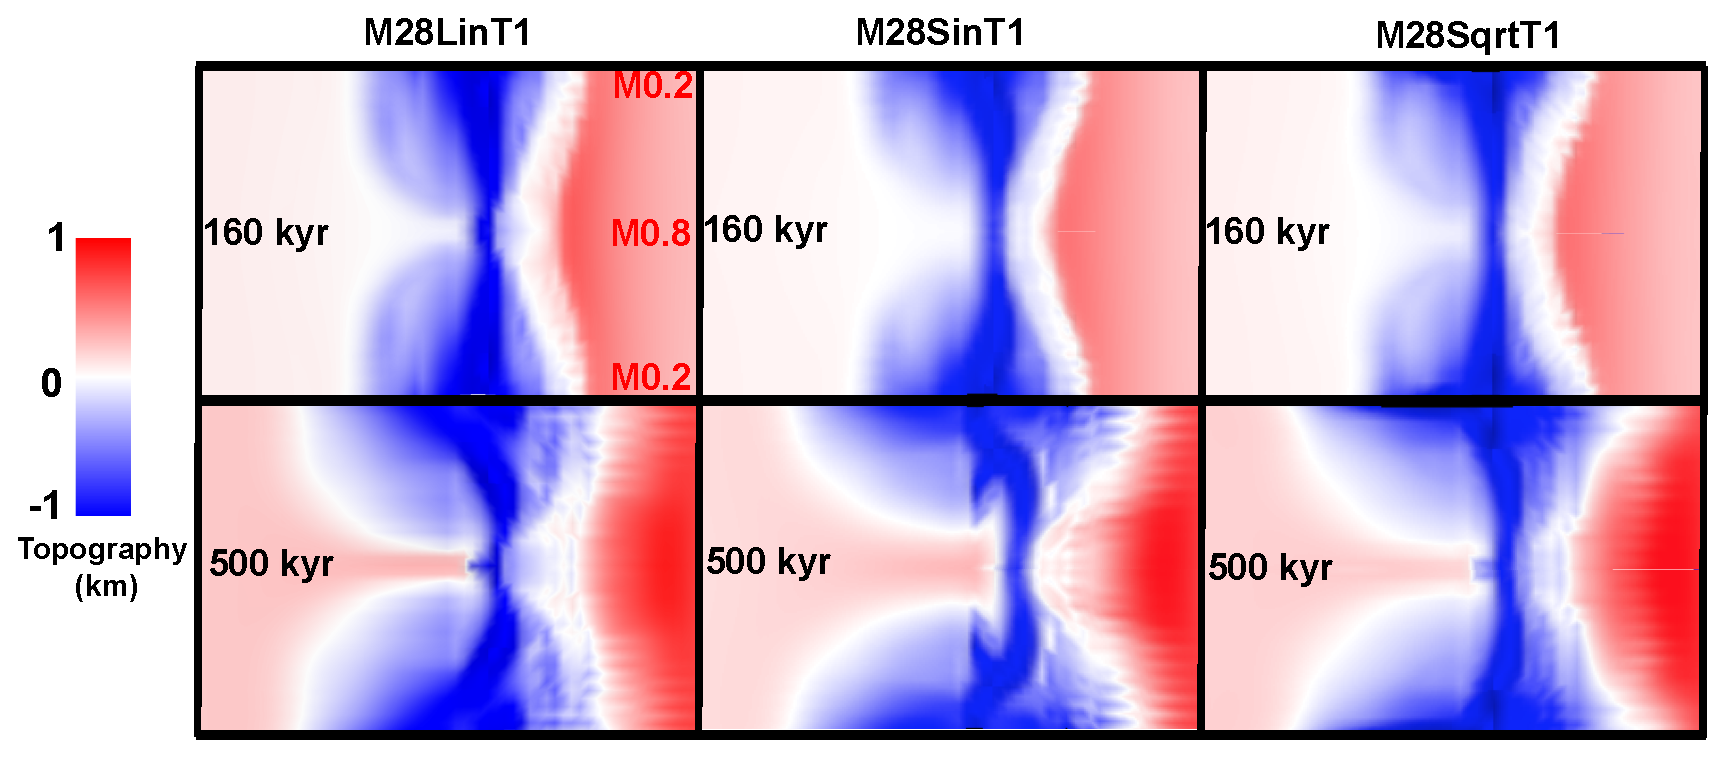
\includegraphics[width=1.0\textwidth]{./Figures/fig_Results_3_3_1_hourglass.eps}
  \caption{Bird's-eye view of the topograpy. (without vertical exaggeration.)}
 \label{fig_Results_3_3_1_hourglass}
\end{figure} 

As shown in Figure~\hyperref[fig_Results_3_3_1_hourglass]{\ref{fig_Results_3_3_1_hourglass}}, differences among the three models are identified. At 160 kyr, median valley for M28SinT1 has the smallest cross-section ($x$-$y$) area at the higher M side. While at the lower M side,  M28SqrtT1 has the smallest area of the cross-section. This is because the cross-section area inside the median valley is inversely proportional to the local M value along the ridge. Moreover, the breakaways at the lower M sides for M28LinT1 and M28SinT1 bend to parallel to the ridge axis while the breakaway for M28SqrtT1 extends further away from the ridge axis. In addition, M28SinT1 has a trough inside the median valley with the highest curvature. At 500 kyr, M28SinT1 has the narrowest median valley at the higher M side and the high topography zone on the left hand side of the ridge axis is the widest. Integrating the topography at the left hand side of the ridge axis of the three models, M28Sqrt has the largest value of integration since it has the largest integration of M along the ridge axis. In addition, the termination of the detachment fault of M28SqrtT1 has the highest curvature at the lower M sides. All these observations correspond to the M variation (Figure~\hyperref[fig_Results3_1]{\ref{fig_Results3_1}}).

\subsubsection{M58(Lin,Sin,Sqrt)T2}

\begin{table}[h!]
\begin{small}
\begin{center}
\begin{tabular}{|l|p{1.2cm}|p{1.2cm}|p{1.2cm}|}
\hline
\diagbox[width=8em]{Function}{M range}&
M28&M57&M58\\
\hline
Linear & \cellcolor{magenta!60}0.4850 & \cellcolor{magenta!60}0.5950 & \cellcolor{magenta!80}0.6425 \\
\hline
Sinusoidal & \cellcolor{magenta!60}0.5668 & \cellcolor{magenta!60}0.6223 & \cellcolor{green!60}0.6834   \\
\hline
Square root & \cellcolor{magenta!60}0.5837 & \cellcolor{magenta!60}0.6279 & \cellcolor{green!60}0.6918  \\
\hline
\end{tabular}
\end{center}
\end{small}
\caption{Average M values of the 20 km segment. (The value is calculated by integrating M along the ridge axis and divided by the length of the model domain in $z$-axis.)}
\label{Tab_3_3_average_M}
\end{table}

Among M58LinT2, M58SinT2 and M58SqrtT2, the major difference lies in whether it has ``fault alternation''. Except for the constant M model M88ContT2, among all the models, only the models with type 2 weakening and M ranges from 0.5 to 0.8 (M58) have fault alternation. However, M58LinT2 does not produces alternating fault during the 1.1 Myr model time. Instead, one detachment fault lasts until $\sim$300 kyr when the inward fault jump happens at the higher M side (0.65 $<$ M $<$ 0.8) and replaces the initial detachment fault. This provides an upper limit of average M value of the whole segment that prevent fault alternation and alows a long-lived detachment fault to produce a OCC. As shown in Table~\hyperref[Tab_3_3_average_M]{\ref{Tab_3_3_average_M}}, the upper limit for the average M value is 0.6425 for M58LinT2. Detail analysis of the fault alternation is given in ``Discussion''.

\subsection{Effects of the weakening rate}

Among the twelve 3D models, three pairs of models have both type 1 and type 2 weakening while the range of M and functional form are maintained to be the same. They are M57SinT1/T2, M58SinT1/T2 and M58SqrtT1/T2.

\subsubsection{M57SinT1 versus M57SinT2}

\begin{figure}[h]
 \centering
  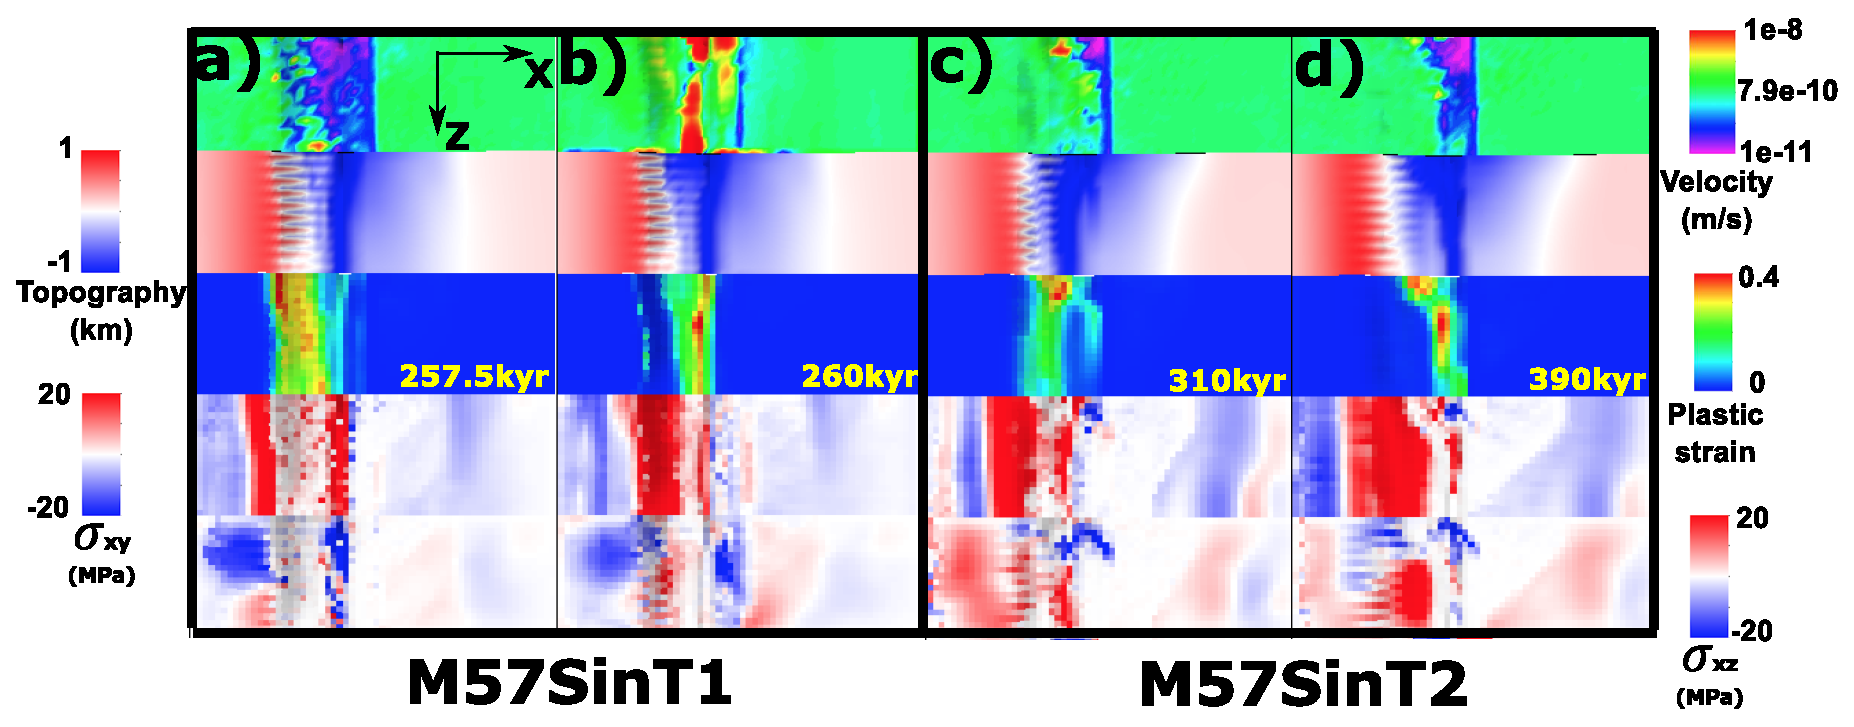
\includegraphics[width=1.0\textwidth]{./Figures/fig_Results_Weakening_2_M57SinT1VST2_CutbackVSsecondaryFault.eps}
 \caption{M57SinT2 versus M57SinT1 (Table~\hyperref[Tab1_1]{\ref{Tab1_1}})}
\label{fig_Results_Weakenging_2}
\end{figure}
~\\
Initially, both models develop normal faults on both sides of the ridge axis at the lower M side. In the model with the faster weakening rate (M57SinT1), faults propagate toward the higher M side and cut through the whole crust by 25 kyr but this process completes later by 50 kyr in the model with the slower weakening rate (M57SinT2). By $\sim$310 kyr, the inward fault jump appears at the higher M side (M $>$ 0.55) of M57SinT2 while at where M $<=$ 0.55, the initial fault remains active (Figure~\hyperref[fig_Results_Weakenging_2]{\ref{fig_Results_Weakenging_2}.c and d}). However, when the weakening is fast (M57SinT1), cut-back happens at $\sim$260 kyr and helps to maintain a relative higher angle fault with a termination closer to the ridge axis. The initial fault remains, no inward fault jump forming (Figure~\hyperref[fig_Results_Weakenging_2]{\ref{fig_Results_Weakenging_2}.a and b}). In addition, the width of median valley at the lower M side is wider for M57SinT2 than M57SinT1 (Figure~\hyperref[fig_Results_Weakenging_2]{\ref{fig_Results_Weakenging_2}.c, d versus a, b}) because slower weakening (type 2) alows a more distributed tensional stress $\sigma_{xx}$ rather than fast weakening that once a fault establishes, larger amount of the tensional stress $\sigma_{xx}$ is released at the fault. The amplitude of the corrugations of M57SinT1 is larger than that of slower weakening M57SinT2. This is because faster weakening rate allows a faster decrease in the cohesion. As the cohesion reaches its minimum of 4 Mpa ealier when the plastic strain accummulates to 0.1, tensile failure is easy to happen in the isochron parallel direction and produces the corrugations.  

\begin{figure}[h]
 \centering
  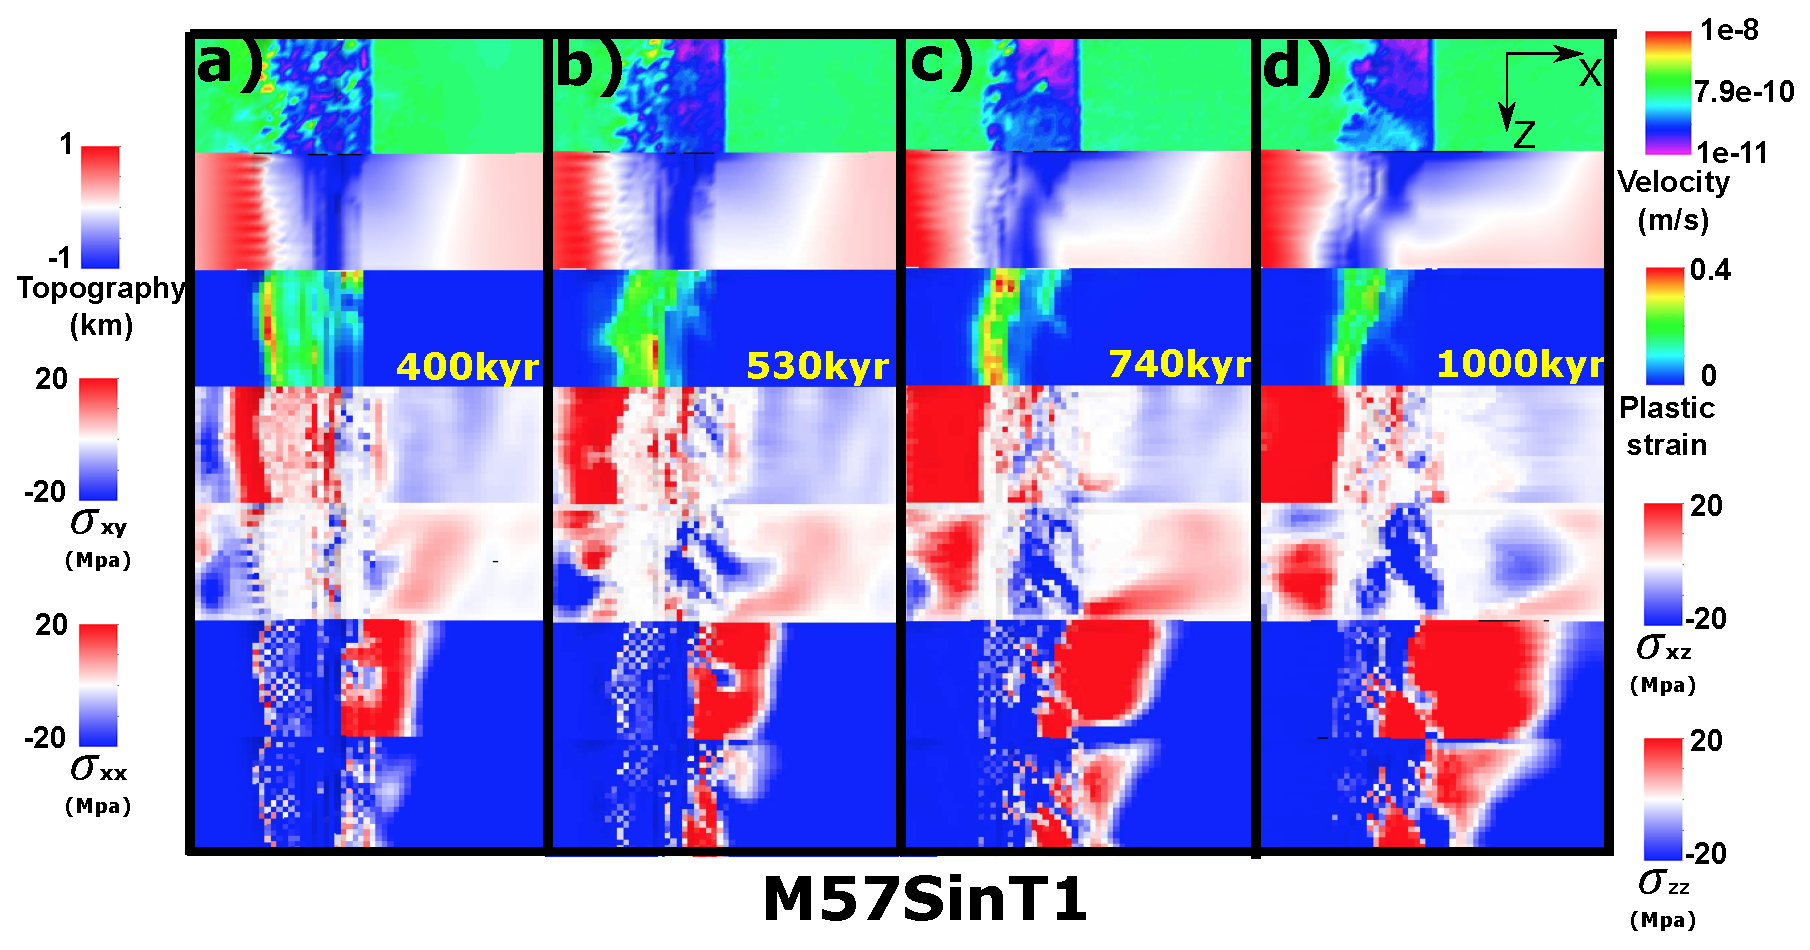
\includegraphics[width=1.0\textwidth]{./Figures/fig_Results_Weakening_3_M57SinT1_time_evolution.eps}
 \caption{Faulting and stress evolution for M57SinT1.}
\label{fig_Results_Weakenging_3}
\end{figure}

\paragraph{M57SinT1}\label{para_M57SinT1}
~\\
For M57SinT1, by 400 kyr (Figure~\hyperref[fig_Results_Weakenging_3]{\ref{fig_Results_Weakenging_3}.a}), two antithetic fault forms at the lower M side (0.5 $<$ M $<$ 0.58) accommodating part of the plates extension. This makes the termination at the lower M side retreat backward to the ridge axis. The hanging walls of the antithetic faults slide down into the trough and lower the topography. By 530 kyr, the termination at the center of the ridge segment (M $=$ 0.61$\sim$0.63) extends further (Figure~\hyperref[fig_Results_Weakenging_3]{\ref{fig_Results_Weakenging_3}.b}). This curved termination leads to a curved topography aligns with it (white curve in the second row). By 740 kyr, another antithetic fault forms at the lower M side (Figure~\hyperref[fig_Results_Weakenging_3]{\ref{fig_Results_Weakenging_3}.c}). It doesn't take the place of initial fault and disapear soon, however, it again releases tensional stress and helps maintain a closer to ridge axis termination at the lower M side. By 1000 kyr (Figure~\hyperref[fig_Results_Weakenging_3]{\ref{fig_Results_Weakenging_3}.d}), an Atlantiss Massif shape OCC is produced (lower M side has a wider dome and higher M side has a narrower dome) due to the along ridge termination evolution. Corrugations with wavelength varying from hundreds to kilometers are also produced.       

\begin{figure}[h]
 \centering
  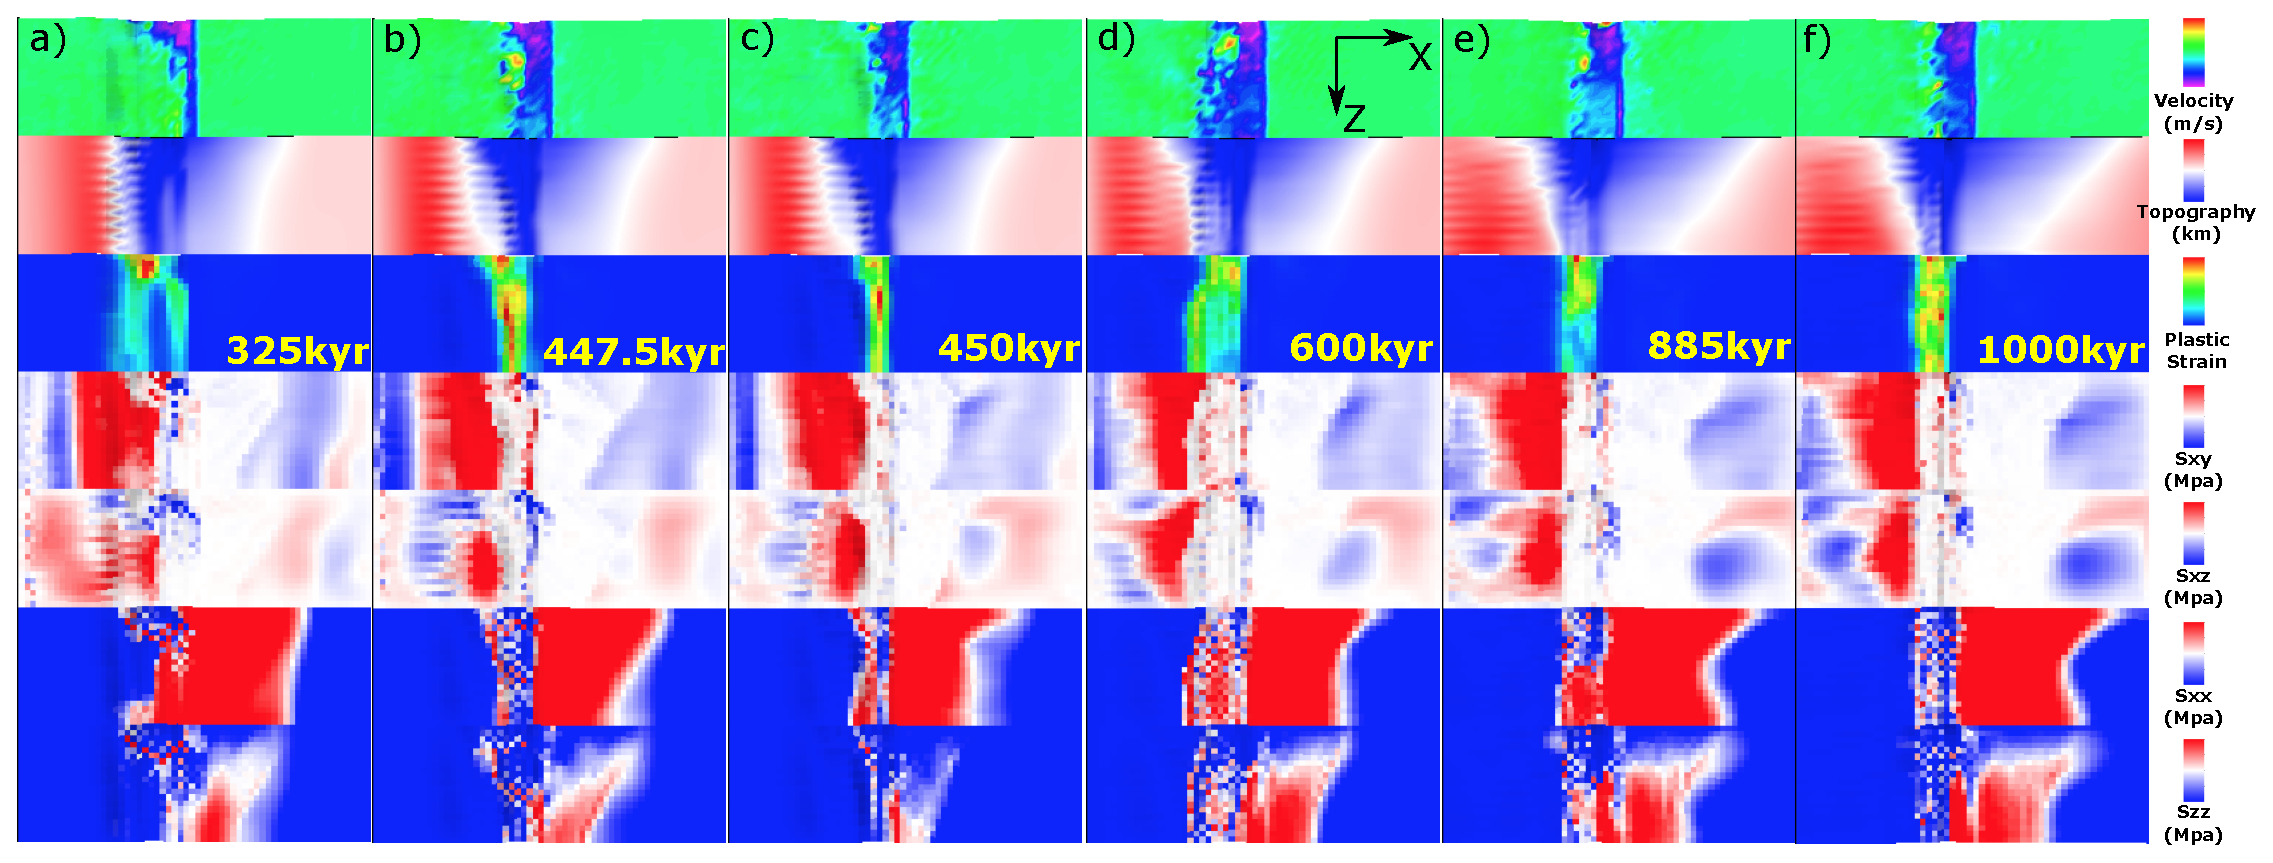
\includegraphics[width=1.0\textwidth]{./Figures/fig_Results_Weakening_4_M57SinT2_time_evolution.eps}
 \caption{M57SinT2 (Table~\hyperref[Tab1_1]{\ref{Tab1_1}}) faulting and stress evolution with respect to time.}
\label{fig_Results_Weakenging_4}
\end{figure}

\paragraph{M57SinT2}\label{para_M57SinT2}
~\\
For M57SinT2, instead of maintaining a detachment fault like M57SinT1, it produces inward fault jump at the higher M side. By 325 kyr (Figure~\hyperref[fig_Results_Weakenging_4]{\ref{fig_Results_Weakenging_4}.a}), an inward fault jump happens and takes the place of the initial detachment fault at the higher M side. Between 447.5 kyr (Figure~\hyperref[fig_Results_Weakenging_4]{\ref{fig_Results_Weakenging_4}.b}) and 450 kyr (Figure~\hyperref[fig_Results_Weakenging_4]{\ref{fig_Results_Weakenging_4}.c}), a small scale cut-back happens and the termination recedes backward. By 600 kyr, the termination at the higher M side extends further (Figure~\hyperref[fig_Results_Weakenging_4]{\ref{fig_Results_Weakenging_4}.d}). By 885 kyr, an inward fault jump happens at the higher M side (0.62 $<$ M $<$ 0.7) (Figure~\hyperref[fig_Results_Weakenging_4]{\ref{fig_Results_Weakenging_4}.e}). The width of the median valley at the lower M side keeps increasing due to the distributed $\sigma_{xx}$ (Figure~\hyperref[fig_Results_Weakenging_4]{\ref{fig_Results_Weakenging_4}.a$\sim$d}).

\subsubsection{M58SinT1 versus M58SinT2}

A major difference between M58SinT1 and M58SinT2 is that only M58SinT2 has fault alternation.

\begin{figure}[h]
 \centering
  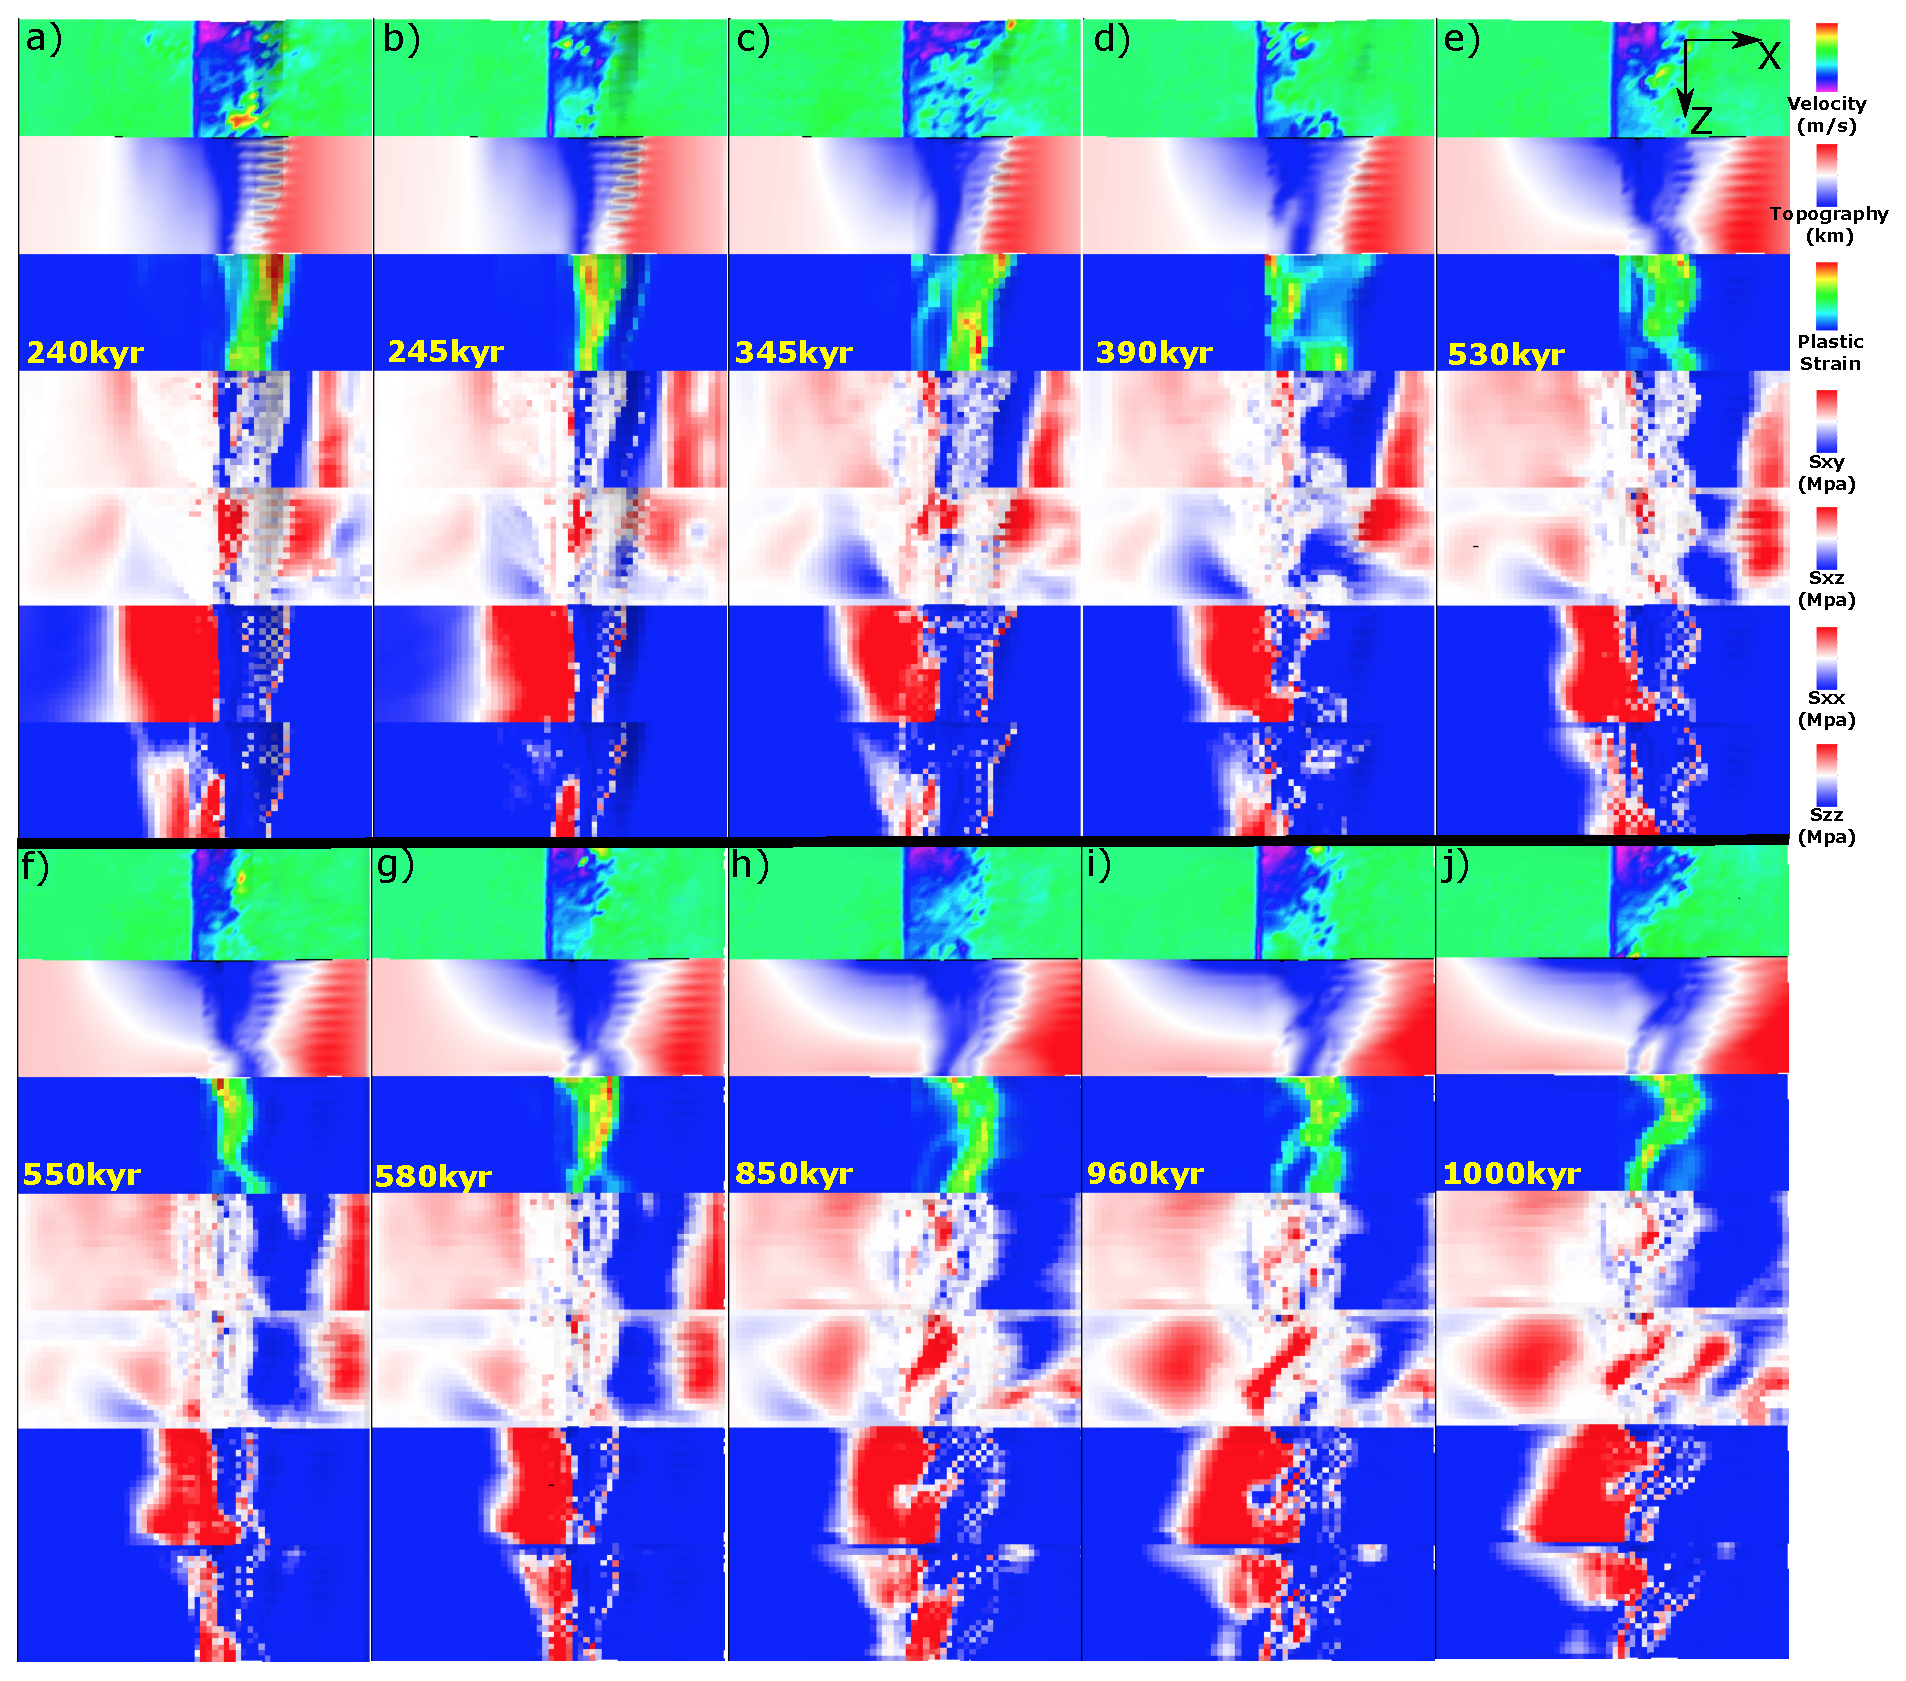
\includegraphics[width=1.0\textwidth]{./Figures/fig_Results_Weakening_5_M58SinT1_time_evolution.eps}
 \caption{Faulting and stresses evolution (M58SinT1).}
\label{fig_Results_Weakenging_5}
\end{figure}

\paragraph{M58SinT1}\label{para_M58SinT1}

\begin{figure}[h]
 \centering
  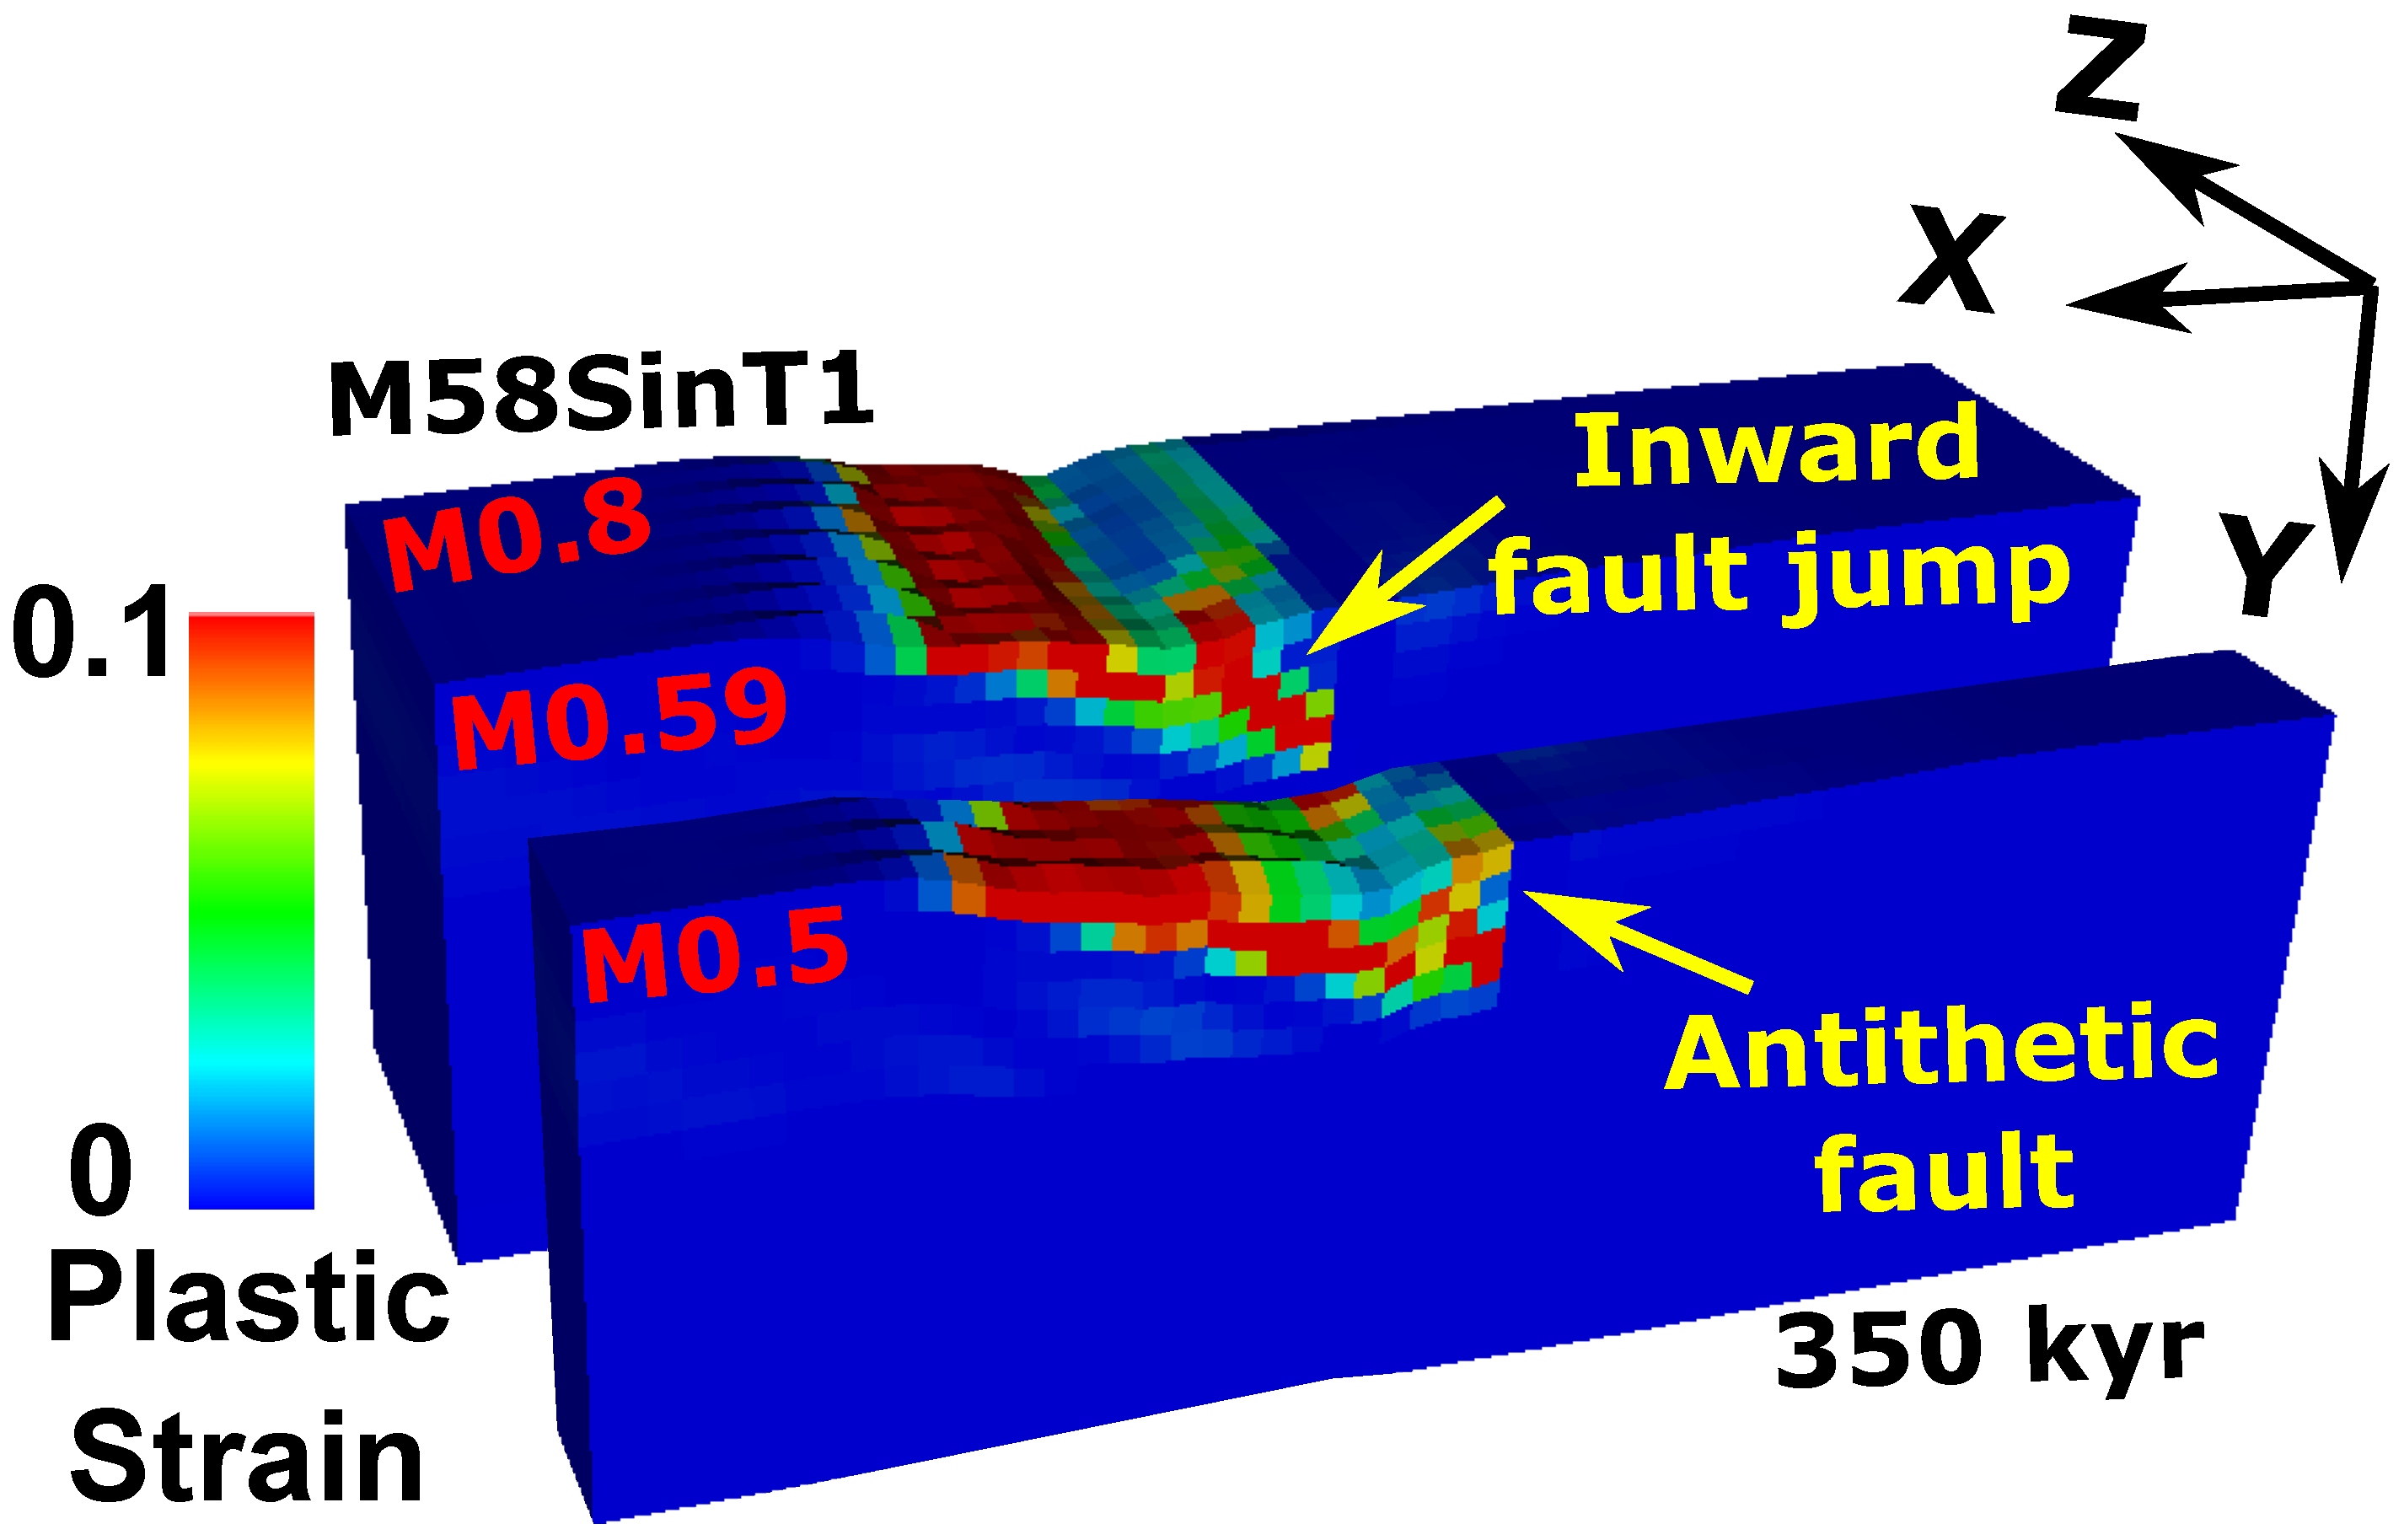
\includegraphics[width=0.6\textwidth]{./Figures/fig_Results_3_4_2_3D_Antithetic_fault.eps}
 \caption{Plastic strain for M58SinT1 at 350 kyr.}
\label{fig_Results_3_4_2_3D_Antithetic_fault}
\end{figure}

~\\
During the 1 Myr extension of the model M58SinT1, 10 phases of the evolution of faulting are identified (Figure~\hyperref[fig_Results_Weakenging_5]{\ref{fig_Results_Weakenging_5}.a$\sim$j}). Antithetic faults, inward fault jumps, cut-backs happens and a rider block, corrugations and mullion structures are produced.

By 240 kyr (Figure~\hyperref[fig_Results_Weakenging_5]{\ref{fig_Results_Weakenging_5}.a}), due to fast weakening (type 1), cohesion along the termination is low. Stress $\sigma_{zz}$ takes the advantage and generates $\sim$2 km wavelength corrugations parallel to the spreading direction as the termination extends further away from the ridge axis. Between 240 kyr (Figure~\hyperref[fig_Results_Weakenging_5]{\ref{fig_Results_Weakenging_5}.a}) and 245 kyr (Figure~\hyperref[fig_Results_Weakenging_5]{\ref{fig_Results_Weakenging_5}.b}), a cut-back happens with mass wasting at the lower M side. The termination recedes toward the ridge axis during the cut-back. By 345 kyr (Figure~\hyperref[fig_Results_Weakenging_5]{\ref{fig_Results_Weakenging_5}.c}), an antithetic fault forms at the lower M side (0.5 $<$ M $<$ 0.545) with an inward fault jump happens at at ridge segment with M $\in$ (0.575, 0.635) (Figure~\hyperref[fig_Results_3_4_2_3D_Antithetic_fault]{\ref{fig_Results_3_4_2_3D_Antithetic_fault}}). 45 kyr later, the two weak zone connect to each other and take the place of the initial detachment fault at the lower M side (Figure~\hyperref[fig_Results_Weakenging_5]{\ref{fig_Results_Weakenging_5}.d}). Due to this inward fault jump, a dextral $\sigma_{xz}$ zone (blue area in the $\sigma_{xz}$ panel) forms and is bounded by the termination of the inward fault jump near the ridge axis at the lower M side and the termination of the initial detachment fault at the higher M side. By 530 kyr (Figure~\hyperref[fig_Results_Weakenging_5]{\ref{fig_Results_Weakenging_5}.e}), the termination of the inward fault jump at the lower M side evolves to a curve with its center extends further away from the ridge axis because the inward fault jump initiates at the center and starts extending away from the ridge axis earlier, however, the lower M side of the curve remains closer to the ridge axis due to the antithetic fault and the other end of the curve is also closer to the ridge axis because the fault initiates later. This curved termination at the lower M side also connects to the initial detachment fault at the higher M side which is further away from the ridge axis. Together, the curved termination is like a mirror reflected letter ``S''. This flipped ``S'' shape termination is also reflected in topography. As the curved termination at the higher M side lasts for $\sim$300 kyr since $\sim$390 kyr, following the shape, a $\sim$10 km in wavelength and $\sim$7 km in along spreading direcion mullion structure is formed (Figure~\hyperref[fig_Results_3_4_2_M58SinT1_mullion_riderBlock_inwardFaultJump]{\ref{fig_Results_3_4_2_M58SinT1_mullion_riderBlock_inwardFaultJump}}). By $\sim$680 kyr, an inward fault jump hapens at the higher M side (0.74 $<$ M $<$ 0.8). It perturbs the curved shape termination and ceases the further exhumation of the mullion structure. This inward fault jump also produces a rider block that covers the inactive detachment fault and moves off axis following the exhuming footwall of the inward jumped fault.

\begin{figure}[h]
 \centering
  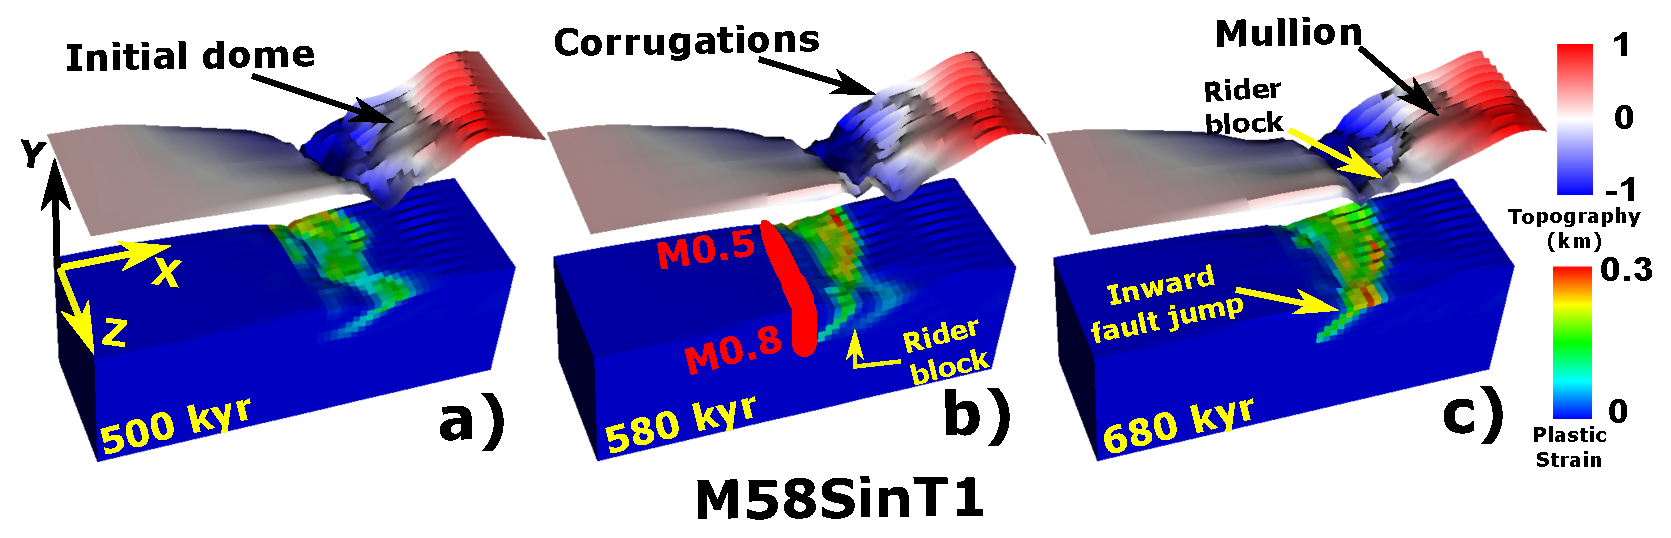
\includegraphics[width=1.0\textwidth]{./Figures/fig_Results_3_4_2_M58SinT1_mullion_riderBlock_inwardFaultJump.eps}
 \caption{Evolution of faulting and morphologies of M58SinT1.}
\label{fig_Results_3_4_2_M58SinT1_mullion_riderBlock_inwardFaultJump}
\end{figure}

Between 530 kyr (Figure~\hyperref[fig_Results_Weakenging_5]{\ref{fig_Results_Weakenging_5}.e}) and 550 kyr (Figure~\hyperref[fig_Results_Weakenging_5]{\ref{fig_Results_Weakenging_5}.f}), another cut-back happens at the lower M side (0.5 $<$ M $<$ 0.545) where a slump block with an area of $\sim$9 km$^{2}$ flows down the topography slope into the trough. Terminations recedes backward to the ridge axis. By 580 kyr, termination at the lower M side extends further away from the ridge axis due to less magma supply. Between 580 kyr and 850 kyr, due to two antithetic faults at the lower M side (M $\in$ (0.5, 0.53) $\cup$ (0.56, 0.605)), the termination at the lower M side recedes and the previous mirror reflected ``S'' shape termination evolves to a half circle curve (Figure~\hyperref[fig_Results_Weakenging_5]{\ref{fig_Results_Weakenging_5}.h}). The shape is also reflected in the topography. By 960 kyr (Figure~\hyperref[fig_Results_Weakenging_5]{\ref{fig_Results_Weakenging_5}.i})), at the ridge segment with M $\in$ (0.62, 0.665), another inward fault jump replaces the detachment fault away from the ridge axis and retreats the termination backward to the ridge axis forming two half circle curves with wavelengths of around half of the model domain in $z$-axis. A large sinistral shear zone (red region $\sim$40 $\degree$ oblique to ridge axis) is seen in the $\sigma_{xz}$ panel. The shear stress $\sigma_{xz}$ results from the inward fault jump at the center of the ridge segment that previous hanging wall changes to the footwall of the inward jumped fault and generates a offset between the old hangingwall at the lower M end and the new footwall of the inward jumped fault. By 1000 kyr, due to the along ridge coupling, the inward fault jump propogates to the higher M side (Figure~\hyperref[fig_Results_Weakenging_5]{\ref{fig_Results_Weakenging_5}.j}). 

\paragraph{M58SinT2}\label{para_M58SinT2}

\begin{figure}[h]
 \centering
  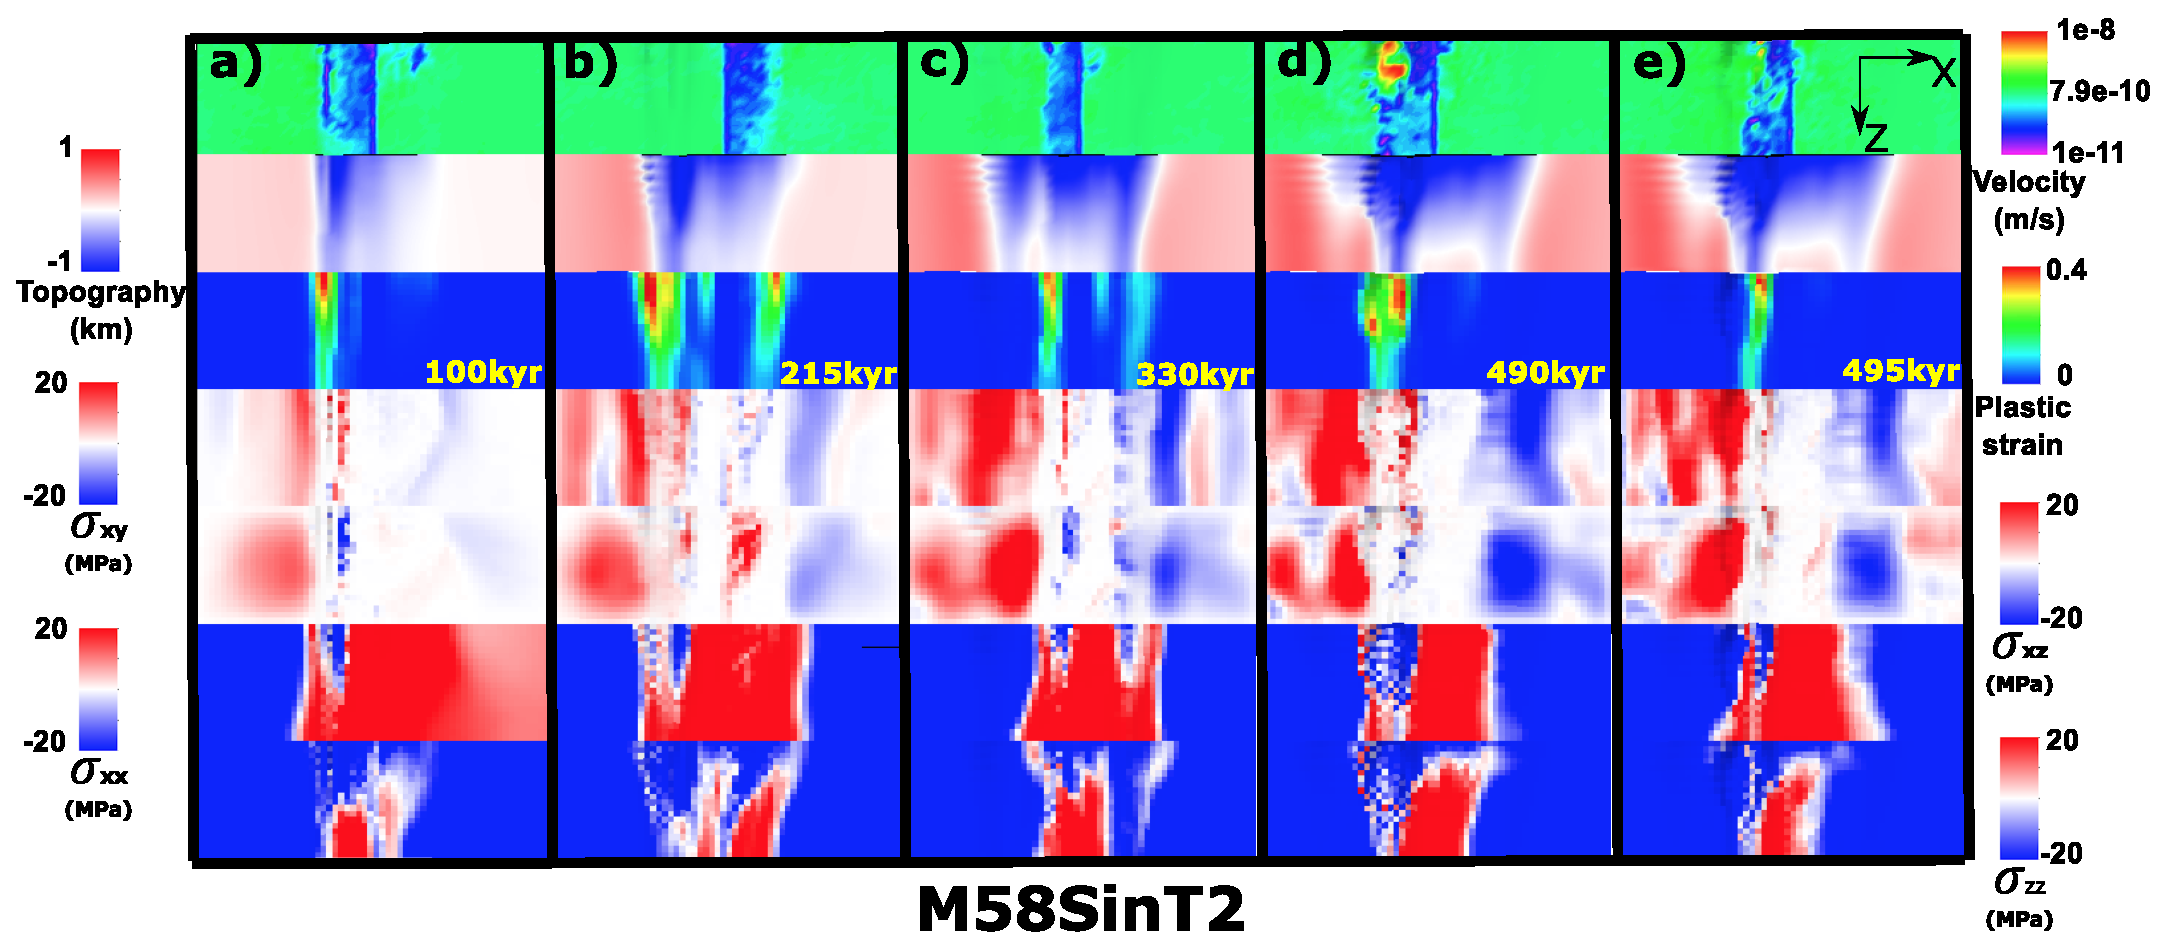
\includegraphics[width=1.0\textwidth]{./Figures/fig_Results_Weakening_6_M58SinT2_time_evolution.eps}
 \caption{Faulting and stresses evolution of M58SinT2.}
\label{fig_Results_Weakenging_6}
\end{figure}

~\\
As shown in Figure~\hyperref[fig_Results_Weakenging_6]{\ref{fig_Results_Weakenging_6}}, a fault initiates on the left hand side of the ridge axis (Figure~\hyperref[fig_Results_Weakenging_6]{\ref{fig_Results_Weakenging_6}.a}). The breakaway at the lower M side extends further than that of the higher M side. It takes longer time of $\sim$100 kyr to form a localized fault plane through the whole ridge segment due to the slower rate of weakening (type 2). By 215 kyr (Figure~\hyperref[fig_Results_Weakenging_6]{\ref{fig_Results_Weakenging_6}.b}), fault alternates to the conjugate plate and gradually replaces the initial one. Corrugations are only produced at the lower M side (M $\in$ (0.5, 0.62)). By 330 kyr, fault alternates again. Between 490 kyr (Figure~\hyperref[fig_Results_Weakenging_6]{\ref{fig_Results_Weakenging_6}.d}) and 495 kyr (Figure~\hyperref[fig_Results_Weakenging_6]{\ref{fig_Results_Weakenging_6}.e}), a cut-back happens with mass wasting and termination receding. A slump block of an area of $\sim$16 km$^{2}$ flows down the topography slope into the trough. With fault alternation, the shape of the median valley is no longer an hourglass. However, at the lower M side, the median valley is still wider and deeper. High frequency abyssal hills are produced at the higher M side. In addition, M58SinT2 has a fault alternation frequency of $\sim$150 kyr which is higher than that of M88ConT2. \add[XT]{Reason for this difference needs further discussion.}

\subsubsection{M58SqrtT1 versus M58SqrtT2}

The major difference between M58SqrtT1 and M58SqrtT2 is also whether the normal fault alternates or not.

\paragraph{M58SqrtT1}\label{para_M58SqrtT1}

\begin{figure}[h]
 \centering
  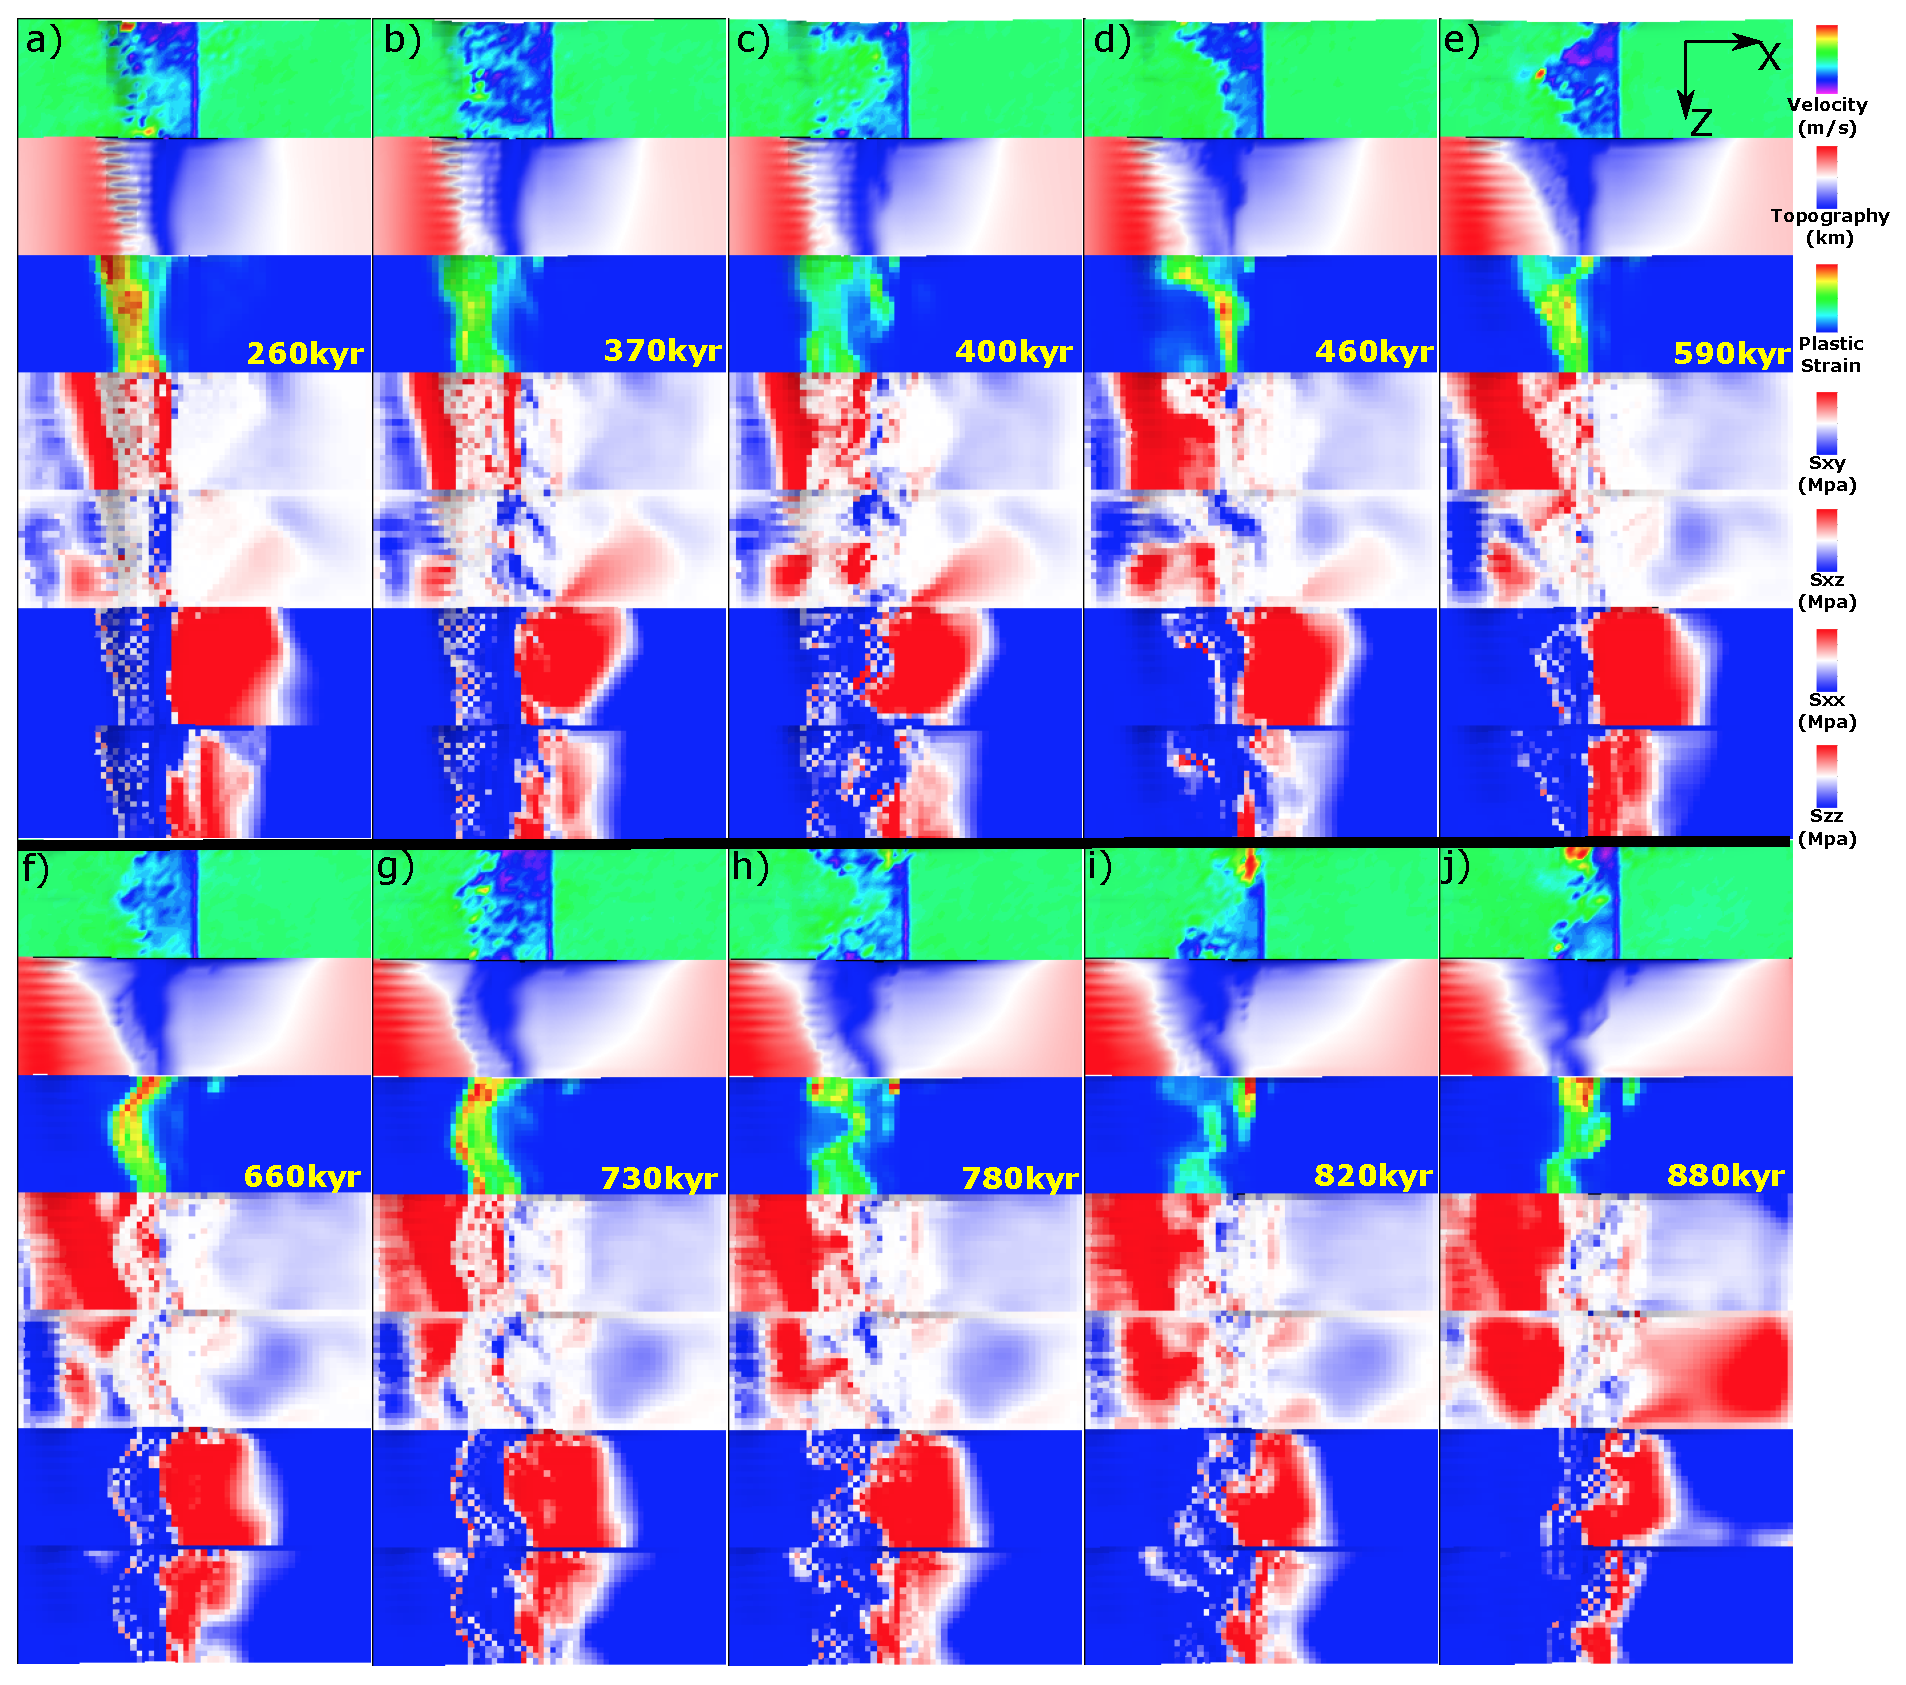
\includegraphics[width=1.0\textwidth]{./Figures/fig_Results_Weakening_7_M58SqrtT1_time_evolution.eps}
 \caption{M58SqrtT1 (Table~\hyperref[Tab1_1]{\ref{Tab1_1}}) faulting and stress evolution with respect to time.}
\label{fig_Results_Weakenging_7}
\end{figure}

~\\
By 260 kyr, breakaway at M $=$ 0.5 extends $\sim$5 km further away from the ridge axis than that of the higher M end (Figure~\hyperref[fig_Results_Weakenging_7]{\ref{fig_Results_Weakenging_7}.a}). Corrugations of a wavelength of $\sim$2 km \add[XT]{2 km is the correct wavelength for corrugations, change previous wrong ones of 1 km} are produced along the ridge. By 370 kyr (Figure~\hyperref[fig_Results_Weakenging_7]{\ref{fig_Results_Weakenging_7}.b}), due to larger value of $\frac{\partial M}{\partial Z}$ at the lower M side, a vertical tensile failure takes place at M $\in$ (0.5, 0.5949)\add[XT]{previous M range for Sin and Sqrt models should be revised, I used linear to calculate with respect to number of elements in Z. Start from this and the later ones are ok} . Two parallel dextral shear stress zones (blue) are seen in the $\sigma_{xz}$ panel. By 400 kyr (Figure~\hyperref[fig_Results_Weakenging_7]{\ref{fig_Results_Weakenging_7}.c}), an inward fault jump happens at where M $\in$ (0.5949, 0.7121) and it propagates to the higher M end and replaces the initial detachment fault at the higher M side by 460 kyr (Figure~\hyperref[fig_Results_Weakenging_7]{\ref{fig_Results_Weakenging_7}.d}). By 590 kyr (Figure~\hyperref[fig_Results_Weakenging_7]{\ref{fig_Results_Weakenging_7}.e}), an inward fault jump happens at the lower M side (M $<$ 0.5949) and connect with the normal fault at the higher M side replacing the initial detachment fault. An $\sim$18 km$^{2}$ triangular shape (bird's-eye view) rider block is produced at the lower M side. Termination at the center of the ridge segment extends furthest away from the ridge axis. This is because the previous inward fault jump first initiates there, so the fault starts slipping earlier and because the value of M is lower at the segment center than the higher M end. By 660 kyr (Figure~\hyperref[fig_Results_Weakenging_7]{\ref{fig_Results_Weakenging_7}.f}), as the previous inward jumped fault at the higher M side evolves, another dome is produced. There is a hint of high angle normal fault at where M $<$ 0.5949 on the conjugate plate. But it doesn't develop. By 730 kyr (Figure~\hyperref[fig_Results_Weakenging_7]{\ref{fig_Results_Weakenging_7}.g}, the termination evolves to a ``half circle'' and the shape is also seen in the topography. By 780 kyr (Figure~\hyperref[fig_Results_Weakenging_7]{\ref{fig_Results_Weakenging_7}.h}), another inward fault jump appears at the ridge segment with M $\in$ (0.6342, 0.7121) and produced a curved termination with a wavelenth of $\sim$10 km. It has the potential to create a large wavelength mullion structure. Meanwhile, at the lower M side (M $<$ 0.5949) near the ridge axis, an antithetic fault forms and propagates toward the higher M side (Figure~\hyperref[fig_Results_Weakenging_7]{\ref{fig_Results_Weakenging_7}.i}). It triggers another inward fault jump to happen at the lower M side and produces another rider block. The inward jumped fault later connects with the detachment fault at the higher M side (Figure~\hyperref[fig_Results_Weakenging_7]{\ref{fig_Results_Weakenging_7}.j}). In addition, a tensile failure shows its hint at the lower M side (M $<$ 0.6342) of the conjugate plate.

\paragraph{M58SqrtT2}\label{para_M58SqrtT2}

\begin{figure}[h]
 \centering
  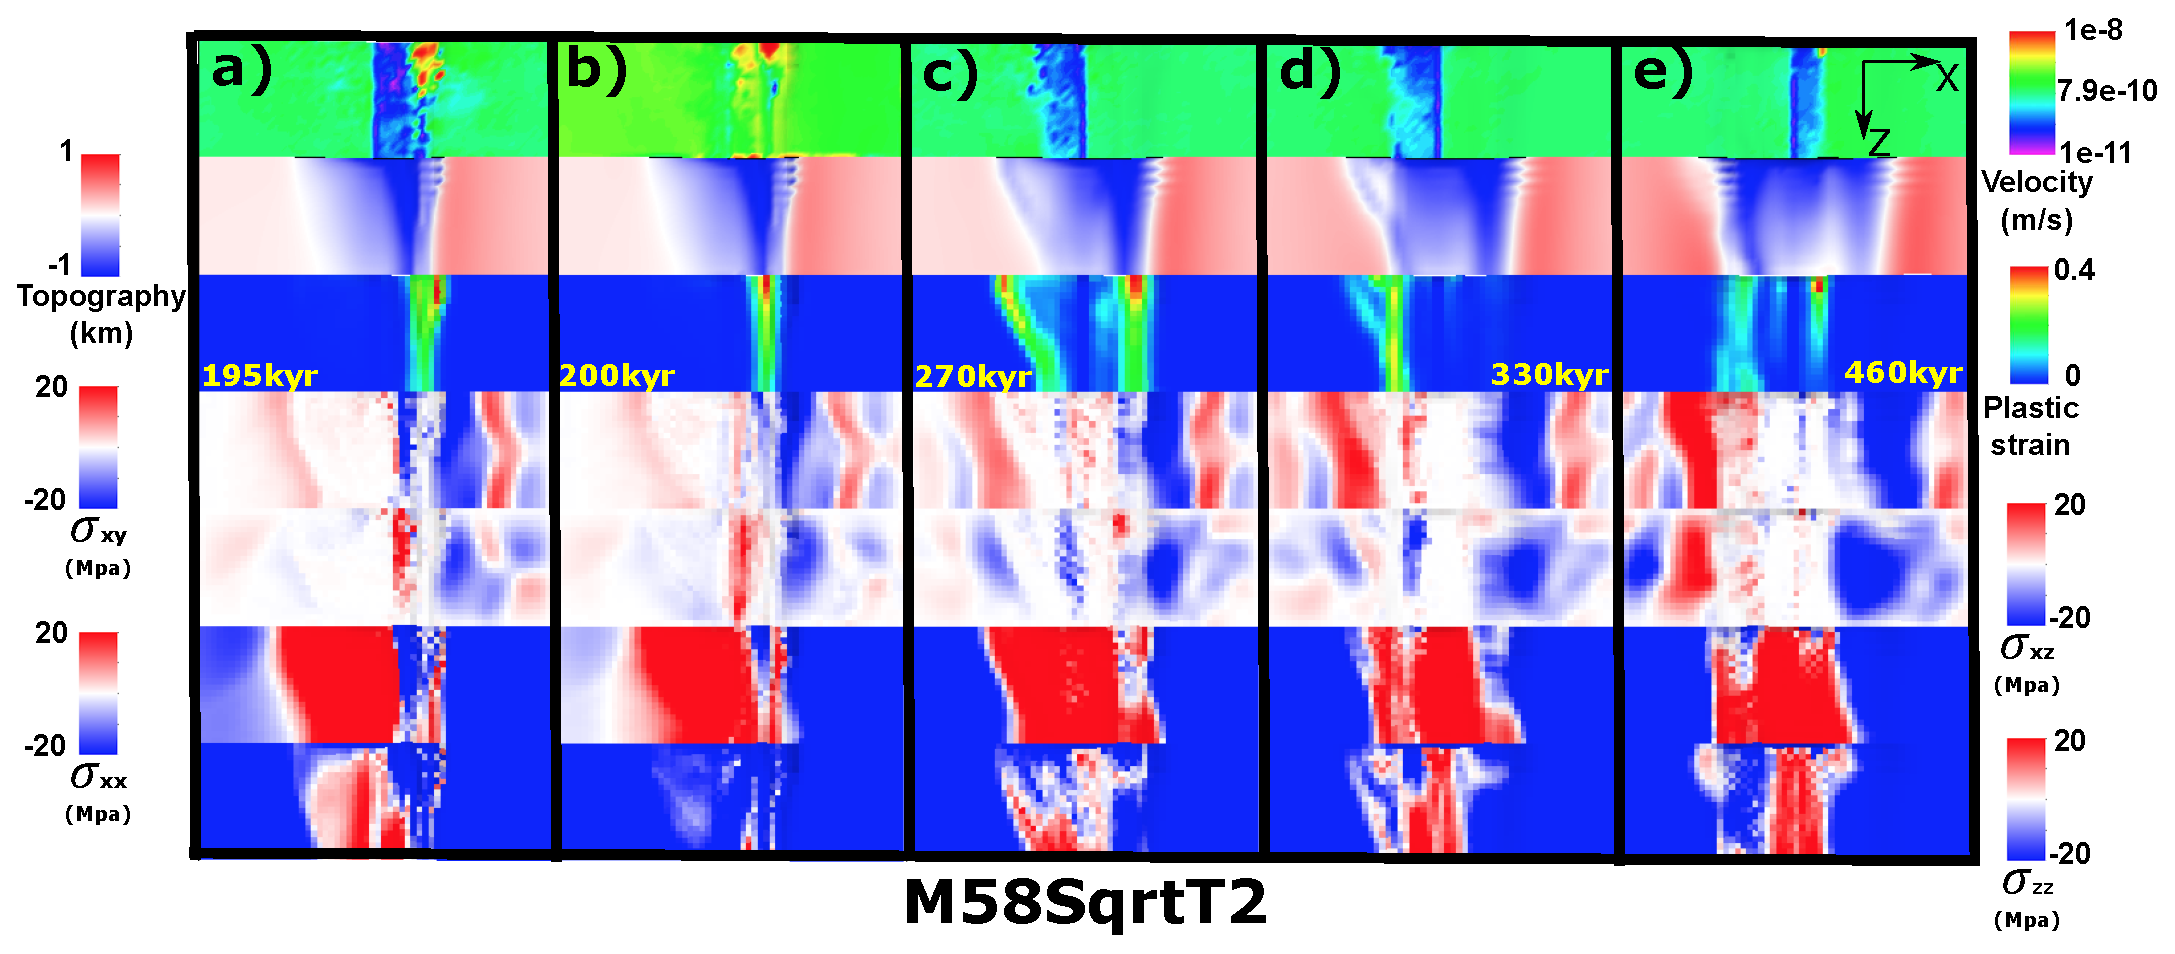
\includegraphics[width=1.0\textwidth]{./Figures/fig_Results_Weakening_8_M58SqrtT2_time_evolution.eps}
 \caption{Faulting and stresses evolution for M58SqrtT2.}
\label{fig_Results_Weakenging_8}
\end{figure}

~\\
By 195 kyr (Figure~\hyperref[fig_Results_Weakenging_8]{\ref{fig_Results_Weakenging_8}.a}), breakaway at the lower M side extends further away from the ridge axis. Three corrugations begin to show up due to tensile failure. Median valley on the conjugate plate is wider at the lower M side because slow weakening allows a more distributed $\sigma_{xx}$ that results in the elastic deppresion of the conjugate plate. Between 195 kyr (Figure~\hyperref[fig_Results_Weakenging_8]{\ref{fig_Results_Weakenging_8}.a}) and 200 kyr (Figure~\hyperref[fig_Results_Weakenging_8]{\ref{fig_Results_Weakenging_8}.b}),  a cut-back happens with mass wasting along the ridge and is followed by the termination retreat. By 270 kyr fault alternates (Figure~\hyperref[fig_Results_Weakenging_8]{\ref{fig_Results_Weakenging_8}.c}). The shape of the alternated fault follows the curved shape shear $\sigma_{xy}$ zone (red) as seen since $\sim$195 kyr on the left hand side of the ridge axis. By 330 kyr (Figure~\hyperref[fig_Results_Weakenging_8]{\ref{fig_Results_Weakenging_8}.d}), at the lower M side, an inward fault jump happens and takes the place of the old fault further away from the ridge axis. By 460 kyr (Figure~\hyperref[fig_Results_Weakenging_8]{\ref{fig_Results_Weakenging_8}.e}), fault alternates again to the right hand side of the ridge axis.

\subsection{Effects of the range of M variation}
Generally, M57 and M58 models create a median valley much narrower and shallower than that of M28 models.

\subsubsection{(M28 M57 M58)SinT1}

\paragraph{M57SinT1 versus M58SinT1}\label{M57SinT1 versus M58SinT1}

~\\
For description of M57SinT1 evolution with respect to time, please refer to Section~\hyperref[para_M57SinT1]{\ref{para_M57SinT1}} and Figure~\hyperref[fig_Results_Weakenging_3]{\ref{fig_Results_Weakenging_3}}. For description of M58SinT1 evolution with respect to time, please refer to  Section~\hyperref[para_M58SinT1]{\ref{para_M58SinT1}} and Figure~\hyperref[fig_Results_Weakenging_5]{\ref{fig_Results_Weakenging_5}}. Comparing M57SinT1 and M58SinT1, the major difference is that the faulting pattern evolution for M58SinT1 is much more dynamic with a higher frequency of inward fault jumps, cut-backs and connection of the offseted fault zones. For M58SinT1, the inward fault jumps and antithetic faults usually replace the old ones. However, for M57SinT1, diking is not strong enough to create big enough stress perturbation along the ridge axis for inward fault jumps or antithetic faults to take the place of the original one. At the lower M side, antithetic faults only help to accommodate tensional stress which assists in maintaining a termination near the ridge axis while the termination at the higher M side gradually moves off axis. This produces an OCC with larger dome at the lower M side than that of higher M side which is opposite to the shape of the OCC produced by M58SinT1. 

\paragraph{M28SinT1}\label{para_M28SinT1}

\begin{figure}[h]
 \centering
  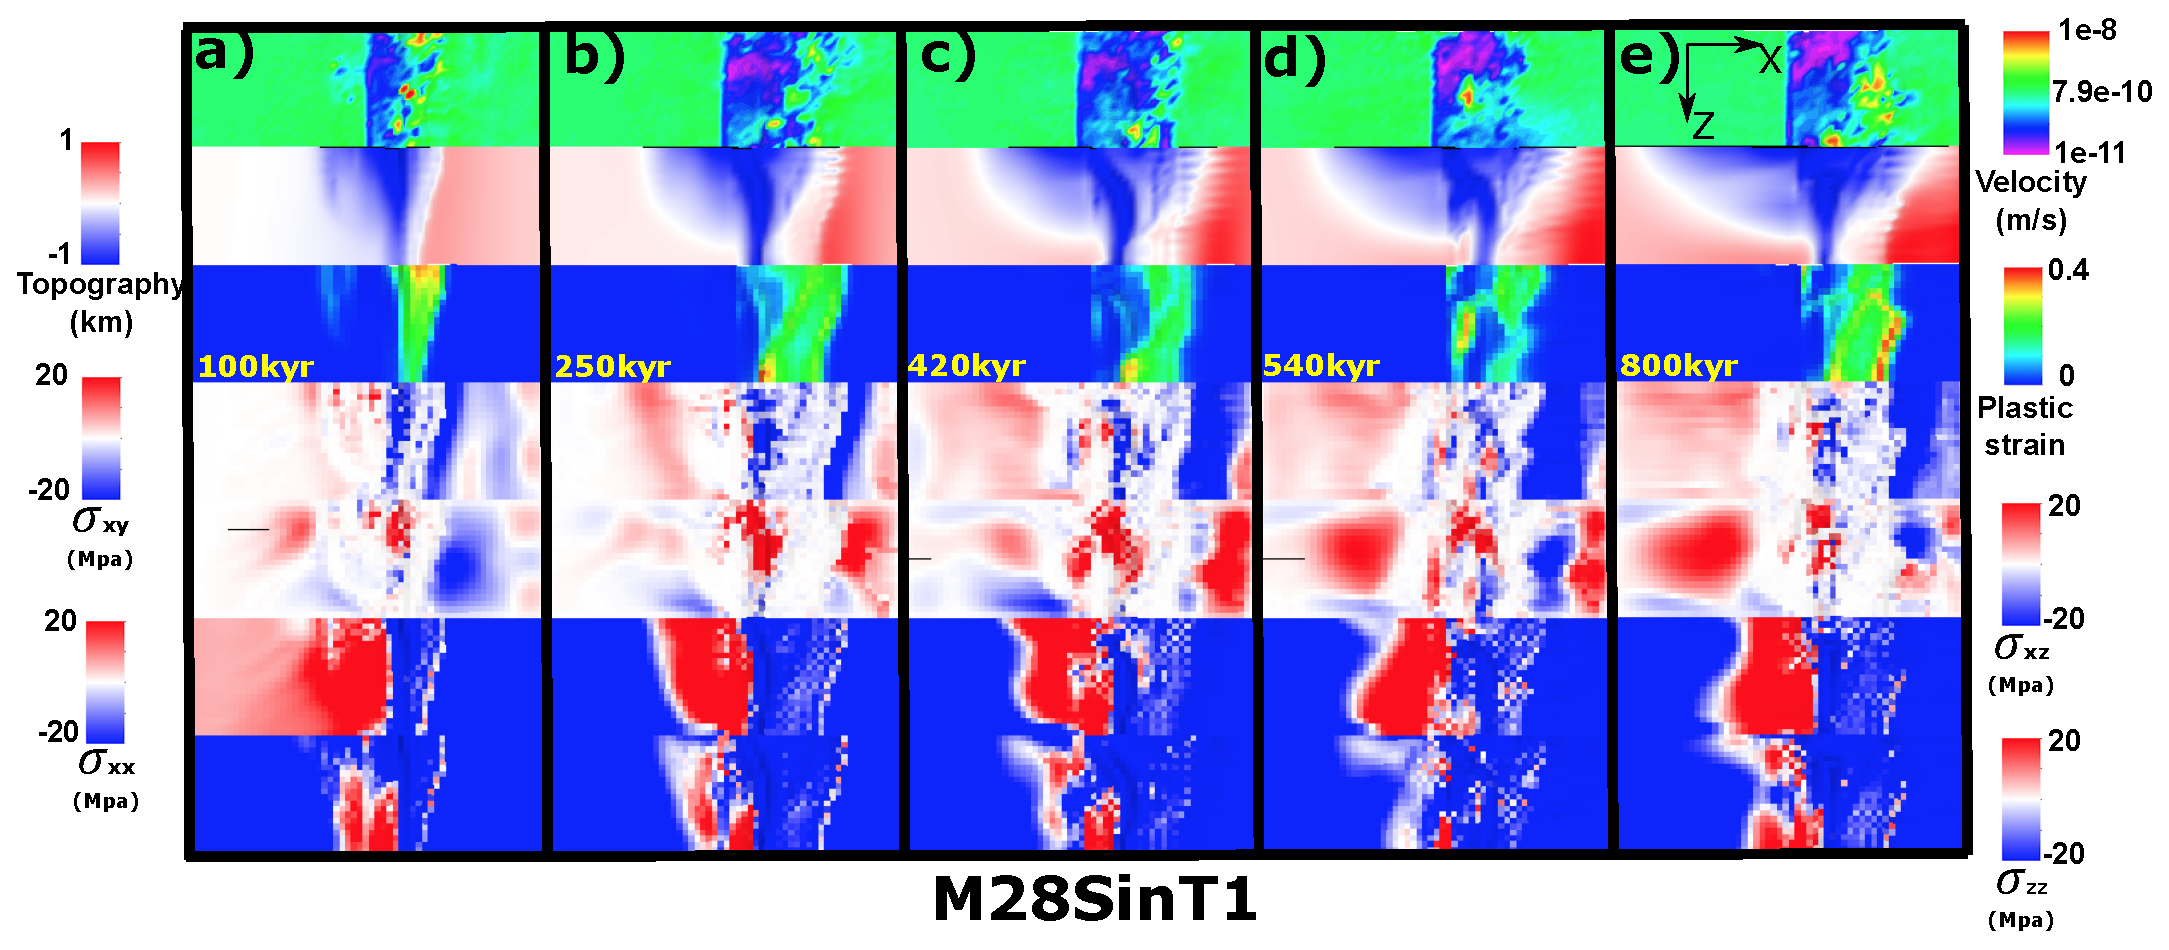
\includegraphics[width=1.0\textwidth]{./Figures/fig_Results_MRange_1_M28SinT1_time_evolution.eps}
 \caption{M28SinT1 (Table~\hyperref[Tab1_1]{\ref{Tab1_1}}) faulting and stress evolution with respect to time.}
\label{fig_Results_MRange_1}
\end{figure}

~\\
As shown in Figure~\hyperref[fig_Results_MRange_1]{\ref{fig_Results_MRange_1}}, faulting evolution is much less dynamic than that of M58SinT1. One detachment fault keeps active on the right hand side of the ridge axis. Only inward fault jump happens $\sim$540 kyr (Figure~\hyperref[fig_Results_MRange_1]{\ref{fig_Results_MRange_1}.d}). By $\sim$100 kyr (Figure~\hyperref[fig_Results_MRange_1]{\ref{fig_Results_MRange_1}.a}), breakaway at the lower M side extends $\sim$4 km further away from ridge axis than the higher M side. By 250 kyr (Figure~\hyperref[fig_Results_MRange_1]{\ref{fig_Results_MRange_1}.b}), $\sim$4 corrugations begin to evolve at the lower M side (M $\in$ (0.2, 0.5135)). By 420 kyr, at the higher M side, a hint of inward fault jump begins to show up. It delvelops into an inward fault jump by 540 kyr (Figure~\hyperref[fig_Results_MRange_1]{\ref{fig_Results_MRange_1}.d}) and propagates toward higher M side. At the lower M side (M $\in$ (0.2, 0.2939)), a tensile failure takes up part of the plate extension and helps maintain a closer to ridge axis termination than the extending termination at the region with M $\in$ (0.4724, 0.6562) (Figure~\hyperref[fig_Results_MRange_1]{\ref{fig_Results_MRange_1}.e}). The curved in termination at the lower M side produces a mullion structure.

\subsubsection{M57SinT2 versus M58SinT2}

For description of M57SinT2 evolution with respect to time, please refer to Section~\hyperref[para_M57SinT2]{\ref{para_M57SinT2}} and Figure~\hyperref[fig_Results_Weakenging_4]{\ref{fig_Results_Weakenging_4}}. For description of M58SinT1 evolution with respect to time, please refer to Section~\hyperref[para_M58SinT2]{\ref{para_M58SinT2}} and Figure~\hyperref[fig_Results_Weakenging_6]{\ref{fig_Results_Weakenging_6}}. A major difference is that M57SinT2 has no fault alternation while M58SinT2 has.

\subsubsection{M28LinT1 versus M57LinT1}

For description of M28LinT1 evolution with respect to time, please refer to Section~\hyperref[sec_M28LinT1]{\ref{sec_M28LinT1}}.

\paragraph{M57LinT1}\label{para_M57LinT1}

\begin{figure}[h]
 \centering
  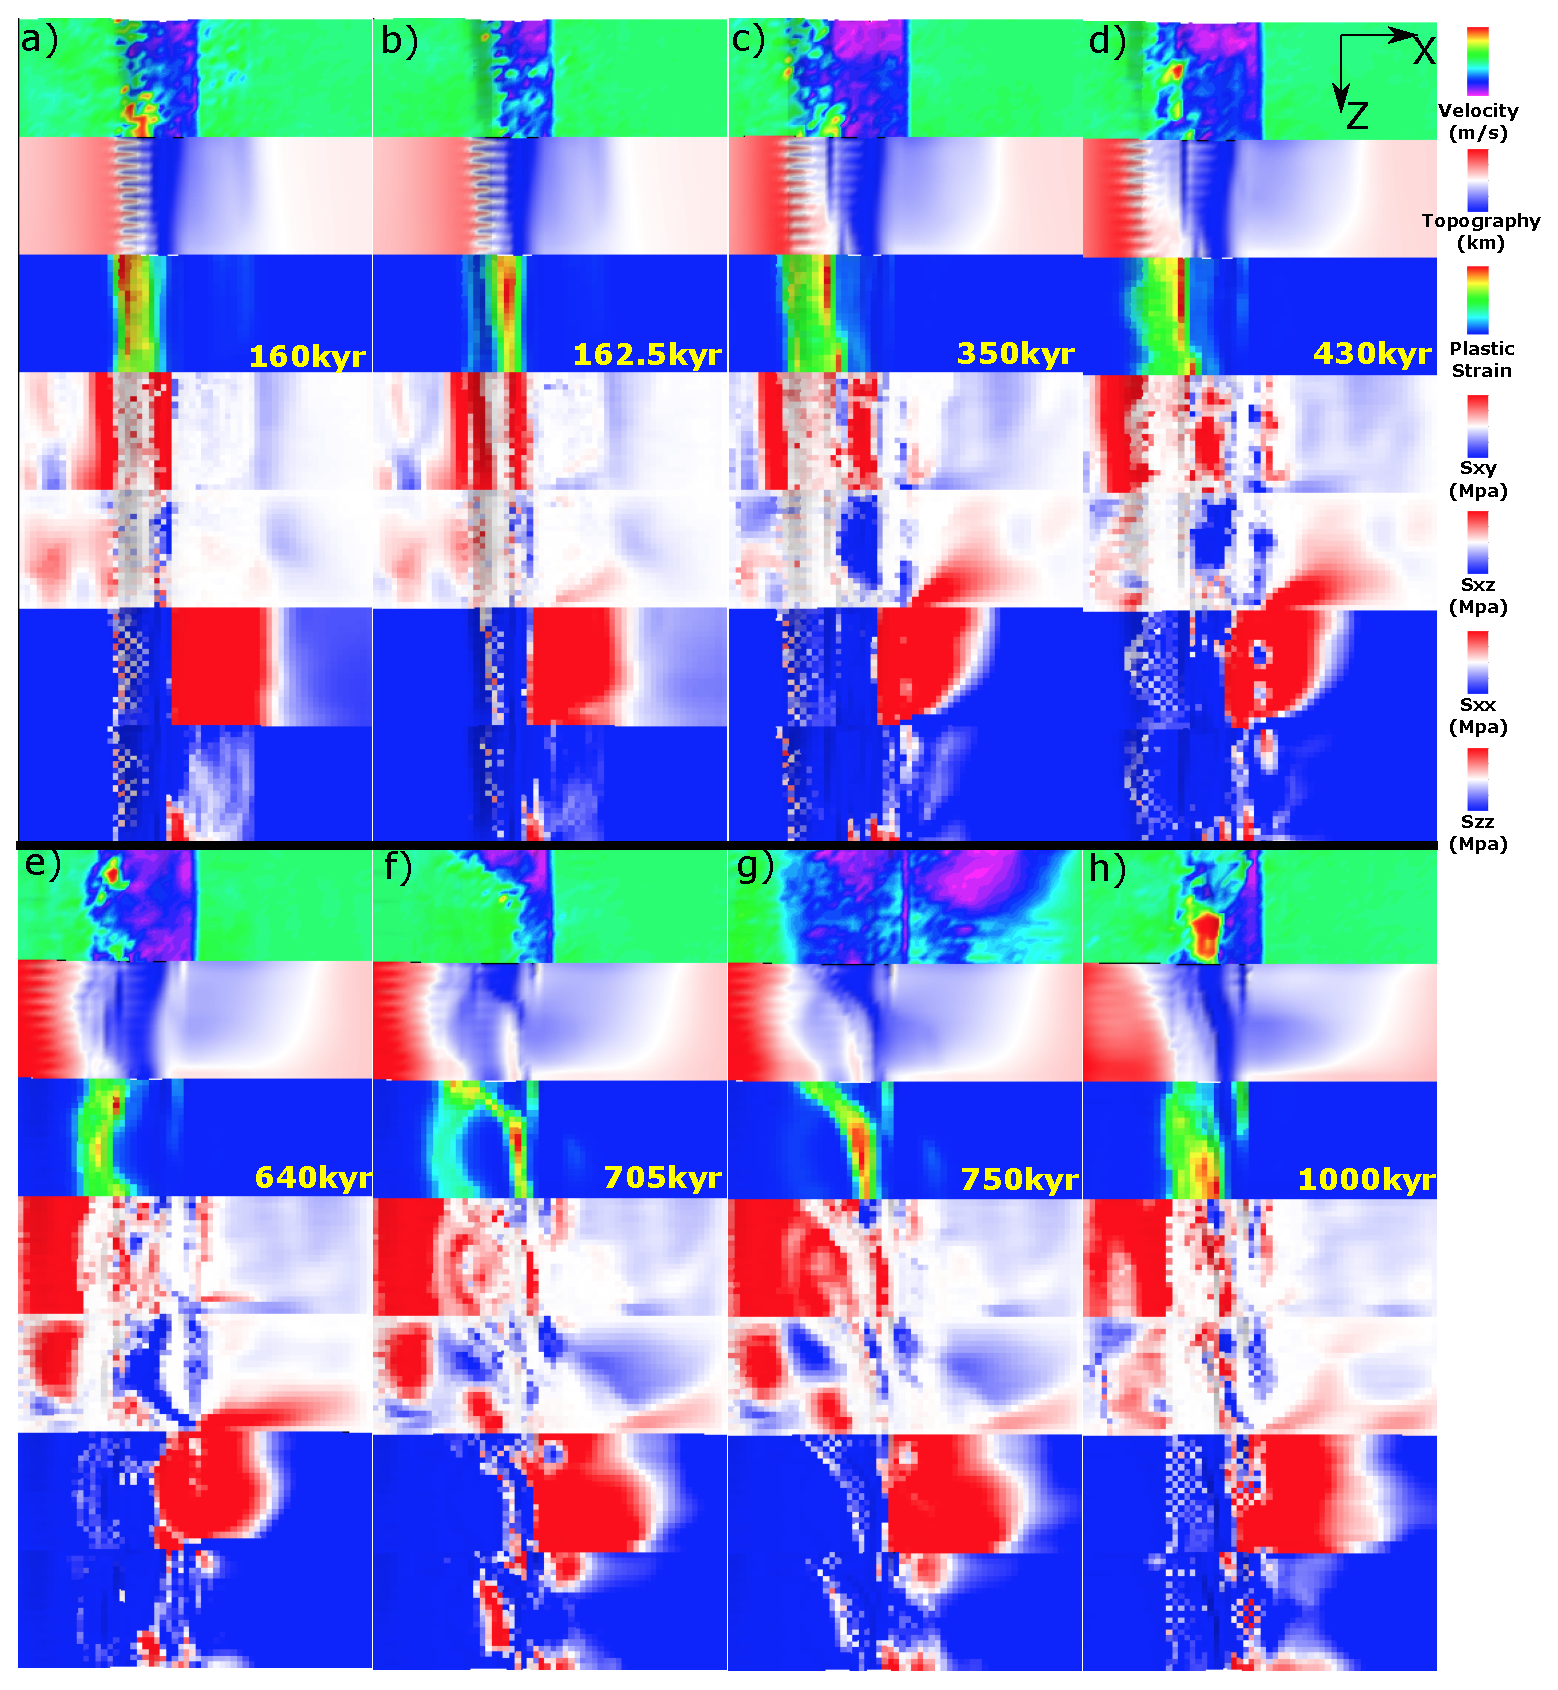
\includegraphics[width=0.8\textwidth]{./Figures/fig_Results_MRange_2_M57LinT1_time_evolution.eps}
 \caption{M57LinT1 (Table~\hyperref[Tab1_1]{\ref{Tab1_1}}) faulting and stress evolution with respect to time.}
\label{fig_Results_MRange_2}
\end{figure}
~\\
As shown in Figure~\hyperref[fig_Results_MRange_2]{\ref{fig_Results_MRange_2}}, between 160 kyr (Figure~\hyperref[fig_Results_MRange_2]{\ref{fig_Results_MRange_2}.a}) and 162.5 kyr (Figure~\hyperref[fig_Results_MRange_2]{\ref{fig_Results_MRange_2}.b}), a cut-back happens. The corrugations have a relatively high amplitude. Due to less M variation (0.2), the along ridge offset in breakaways is smaller. The median valley almost has a constant width along the ridge. By 350 kyr (Figure~\hyperref[fig_Results_MRange_2]{\ref{fig_Results_MRange_2}.c}), a tensile failure happens at the region with M $\in$ (0.5, 0.61) and generates a linear topography low. Another shorter tensile failure at the higher M side (M $>$ 0.64) helps maintain a high angle normal fault near the ridge axis. By 430 kyr (Figure~\hyperref[fig_Results_MRange_2]{\ref{fig_Results_MRange_2}.d}), the tensile failure at the lower M side (M $<$ 0.52) is responsible for the retreat of the termination. While at where M $\in$ (0.54, 0.59), the termination extends further away from the ridge axis. This curved termination results in a ``dog bone'' shape topography as seen at 640 kyr (Figure~\hyperref[fig_Results_MRange_2]{\ref{fig_Results_MRange_2}.e}) and is also responsible for the large dextral shear (blue) stress $\sigma_{xz}$. By 705 kyr (Figure~\hyperref[fig_Results_MRange_2]{\ref{fig_Results_MRange_2}.f}), an inward fault jump happens and replaces the original detachment fault at the higher M side with a length of $\sim$15 km. This inward jumped fault connects with the detachment fault at the lower M side. The new ``L'' shape termination is responsible for the topography seen at 1000 kyr (Figure~\hyperref[fig_Results_MRange_2]{\ref{fig_Results_MRange_2}.h}). The termination at the higher M side soon catches up the further extended termination at the lower M side due to the presence of a tensile failure.
       
\subsubsection{M28SqrtT1 versus M58SqrtT1}

For description of the evolution of M28SqrtT1, please refer to Paragraph~\hyperref[para_CutBack]{\ref{para_CutBack}}. For description of evolution of M58SqrtT1, please refer to Paragraph~\hyperref[para_M58SqrtT1]{\ref{para_M58SqrtT1}}. Generally the faulting evolution for M58SqrtT1 is more dynamic with several inward fault jumps, antithetic faults, connection between offseted faults along the ridge while M28SqrtT1 is simpler with only two cut-backs.

\subsubsection{M57SqrtT2 versus M58SqrtT2}

For description of evolutio of M58SqrtT2, please refer to Paragraph~\hyperref[para_M58SqrtT2]{\ref{para_M58SqrtT2}}.

The major difference between M57SqrtT2 and M58SqrtT2 is that only M58SqrtT2 has fault alternation.

\paragraph{M57SqrtT2}

\begin{figure}[h]
 \centering
  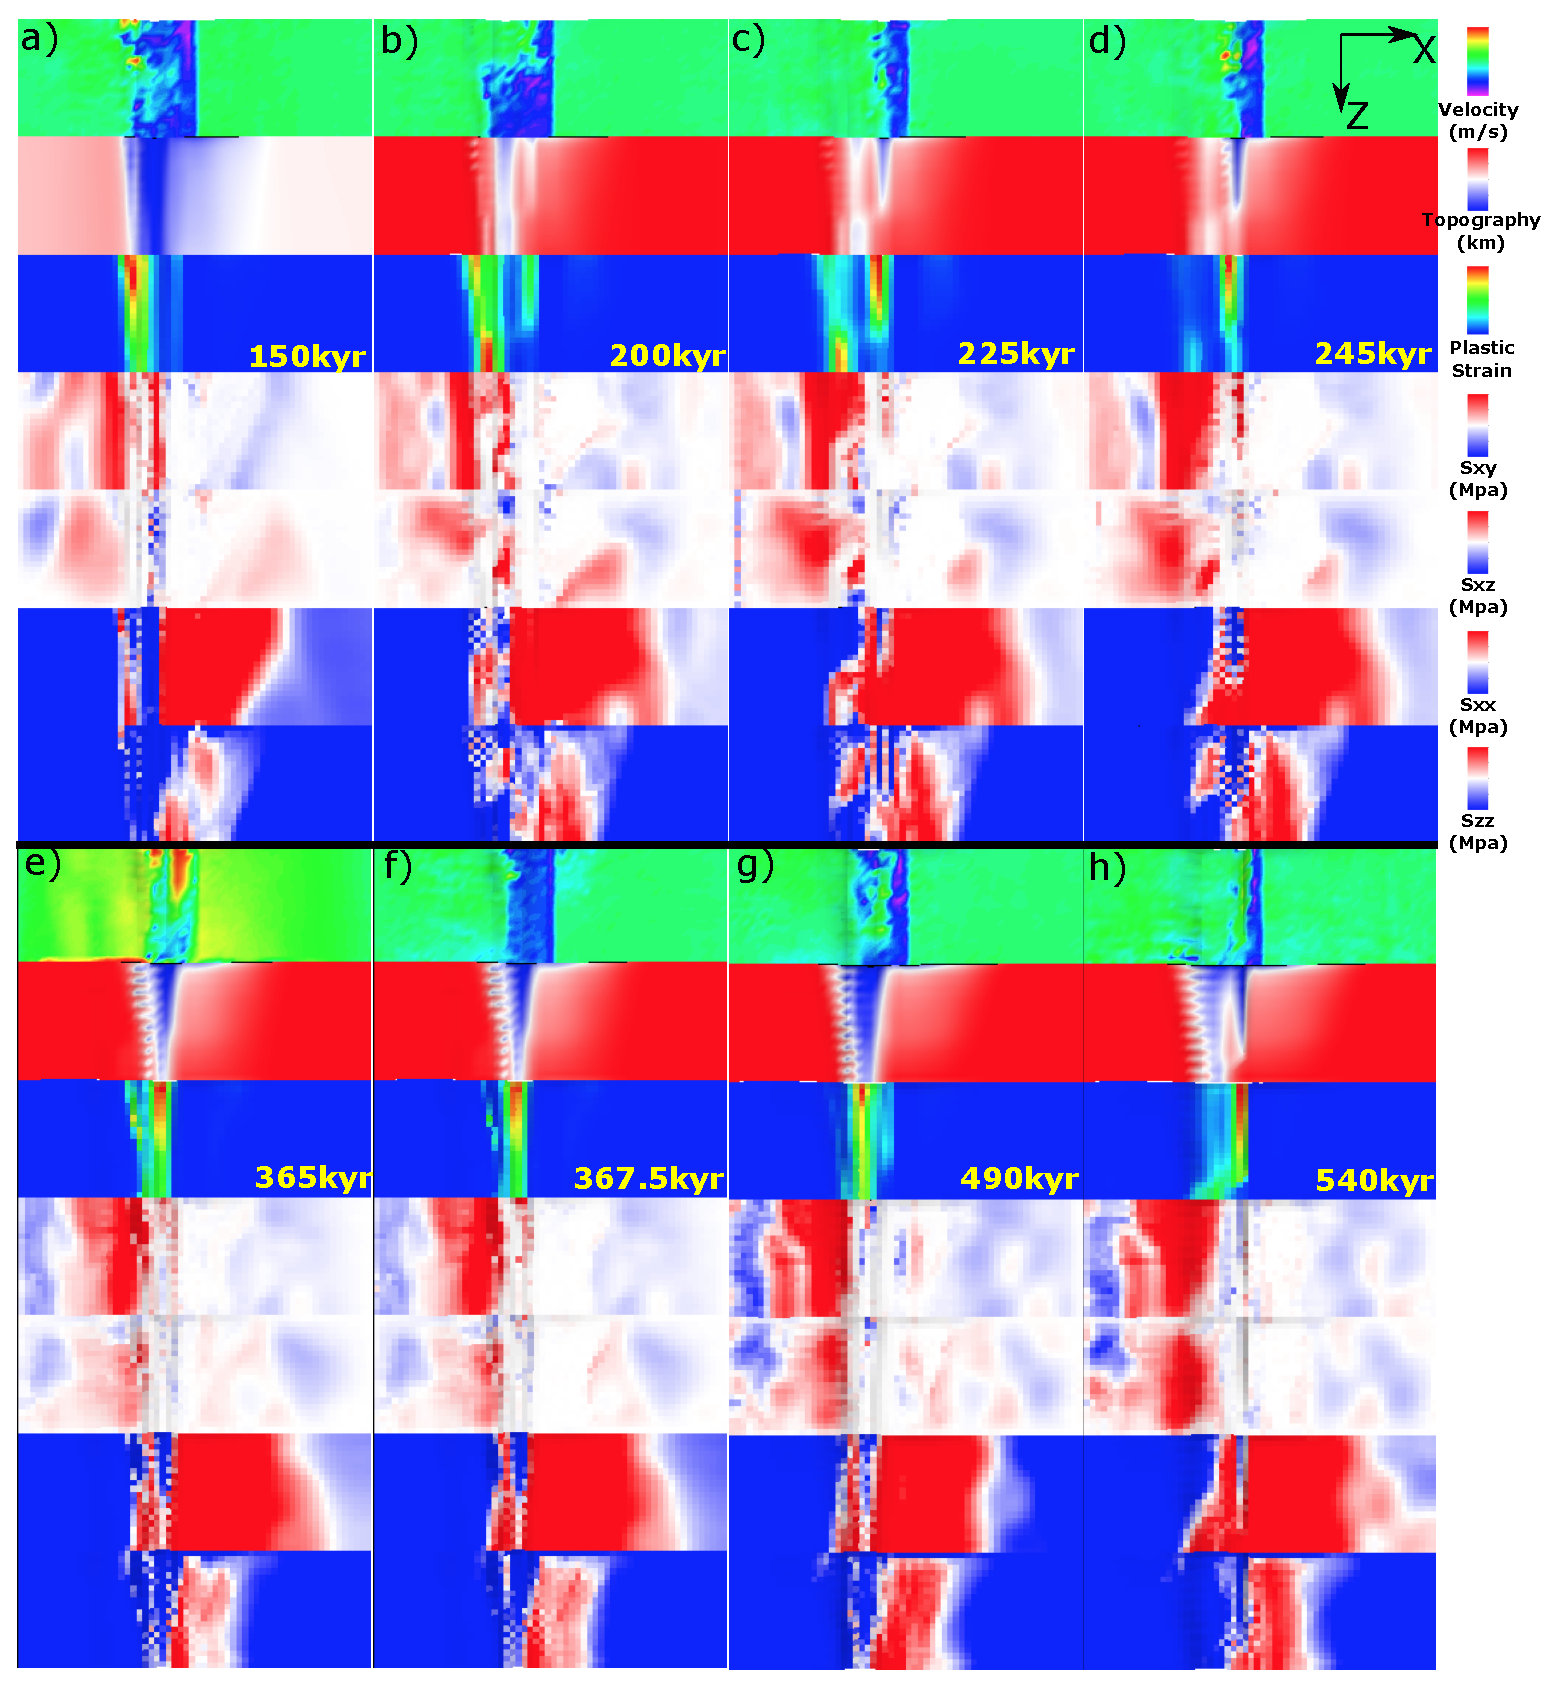
\includegraphics[width=0.8\textwidth]{./Figures/fig_Results_MRange_3_M57SqrtT2_time_evolution.eps}
 \caption{M57SqrtT2 (Table~\hyperref[Tab1_1]{\ref{Tab1_1}}) faulting and stress evolution with respect to time.}
\label{fig_Results_MRange_3}
\end{figure}

~\\
For M57SqrtT2, six small scale cut-back happen at 282.5 kyr, 290 kyr, 365 kyr, 452.5 kyr, 482.5 kyr and 540 kyr respectively. As shown in Figure~\hyperref[fig_Results_MRange_3]{\ref{fig_Results_MRange_3}}, the fault keeps on the left hand side of the ridge axis. By 200 kyr (Figure~\hyperref[fig_Results_MRange_3]{\ref{fig_Results_MRange_3}.b}), an inward fault jump begins to evolve and takes the place of the initial fault. As the fault evolves, a stage of discontinuous abyssal hill is produced at the lower M side (Figure~\hyperref[fig_Results_MRange_3]{\ref{fig_Results_MRange_3}.c}). The fault propagates toward the higher M side and cuts through the plate by $\sim$245 kyr (Figure~\hyperref[fig_Results_MRange_3]{\ref{fig_Results_MRange_3}.d}) when corrugations at the lower M side are produced. Between 365 kyr (Figure~\hyperref[fig_Results_MRange_3]{\ref{fig_Results_MRange_3}.e}) and 367.5 kyr (Figure~\hyperref[fig_Results_MRange_3]{\ref{fig_Results_MRange_3}.f}), a cut-back happens. By 490 kyr (Figure~\hyperref[fig_Results_MRange_3]{\ref{fig_Results_MRange_3}.g}), an antithetic fault begins to evolve and terminates the old fault. It then develops into a vertical tensile failure at 540 kyr (Figure~\hyperref[fig_Results_MRange_3]{\ref{fig_Results_MRange_3}.h}). \add[XT]{for M57SqrtT2, the topography since 200 kyr uplifted, I suspect ther might be some runtime error for this model. Consider to abandon this model and if possible, rerun it. }
